\documentclass[12pt, a4paper]{article}

\usepackage[utf8]{inputenc}
\usepackage[T1]{fontenc}
\usepackage{lmodern}
\usepackage[margin=2.5cm]{geometry}

\usepackage[nosumlimits]{amsmath}
\usepackage{amssymb, stmaryrd, amsthm, MnSymbol}
\usepackage{amsfonts, amsopn}
\usepackage{mathtools}
\usepackage{graphicx}
\usepackage[dvipsnames]{xcolor}
\usepackage[hidelinks]{hyperref}
\usepackage{booktabs}
\usepackage{microtype}
\usepackage{placeins}
\usepackage{float}
\usepackage{bbold}
\usepackage{phoenician}
\usepackage{tikz, tikz-cd}
\usetikzlibrary{arrows.meta, positioning, decorations.pathreplacing}
\usepackage{natbib}
\let\OLDthebibliography\thebibliography
\renewcommand\thebibliography[1]{%
  \OLDthebibliography{#1}%
  \setlength{\parskip}{1pt}%
  \setlength{\itemsep}{0pt plus 0.3ex}%
}
\bibliographystyle{plainnat}

\graphicspath{{images/}}

% colours
\newcommand{\blue}{\color{blue}}
\newcommand{\red}{\color{red}}
\newcommand{\green}{\color{ForestGreen}}
\newcommand{\brickred}{\color{BrickRed}}

% handling simplices
\newcommand{\T}{\mathcal{T}}
\newcommand{\K}{\mathcal{K}}
\newcommand{\V}{\mathcal{V}}
\newcommand{\E}{\mathcal{E}}
\newcommand{\F}{\mathcal{F}}

\newcommand{\simplexname}{\sigma}
\newcommand{\simplex}[3]{\freeQ{\simplexname}{#1}{#2}{#3}}
\newcommand{\simplexnametwo}{\kappa}
\newcommand{\simplextwo}[3]{\freeQ{\simplexnametwo}{#1}{#2}{#3}}
\newcommand{\simplexsubset}[2]{\freeVec{\Delta}{#1}{#2}}

\newcommand{\vertex}[2]{\freeQ{v}{}{#1}{#2}}
\newcommand{\vertexpos}[2]{\freeQ{\Vec{v}}{}{#1}{#2}}
\newcommand{\edge}[2]{\freeQ{e}{}{#1}{#2}}
\newcommand{\face}[2]{\freeQ{f}{}{#1}{#2}}

% adjacency relations
\newcommand{\KmKnl}[3]{\K^{#1}\K^{#2}_{#3}}
\newcommand{\VFl}[1]{\V\F_{#1}}
\newcommand{\EFl}[1]{\E\F_{#1}}
\newcommand{\FFl}[1]{\F\F_{#1}}
\newcommand{\VEl}[1]{\V\E_{#1}}
\newcommand{\EEl}[1]{\E\E_{#1}}
\newcommand{\FEl}[1]{\F\E_{#1}}
\newcommand{\VVl}[1]{\V\V_{#1}}
\newcommand{\EVl}[1]{\E\V_{#1}}
\newcommand{\FVl}[1]{\F\V_{#1}}

\newcommand{\KKltoL}[3]{\K^{#1}\K^{#1}_{#2 \to #3}}
\newcommand{\VVltoL}[2]{\V\V_{#1 \to #2}}
\newcommand{\EEltoL}[2]{\E\E_{#1 \to #2}}
\newcommand{\FFltoL}[2]{\F\F_{#1 \to #2}}

% indices for components
\newcommand{\coarseIdxone}{{\brickred i}}
\newcommand{\coarseIdxtwo}{{\brickred m}}
\newcommand{\fineIdxone}{{\brickred j}}
\newcommand{\fineIdxtwo}{{\brickred n}}

% indices for levels
\renewcommand{\l}{{\green\ell}}
\renewcommand{\L}{{\green L}}
\newcommand{\lzero}{{\green 0}}
\newcommand{\lone}{{\green{\l'}}}
\newcommand{\ltwo}{{\green{\l''}}}
\newcommand{\lthree}{{\green{\l'''}}}

% numbers
\newcommand{\nc}{{\color{Magenta} n_c}}
\newcommand{\nr}{{\color{Magenta} n_r}}
\newcommand{\ns}{{\color{Magenta} n_s}}

% stencils
\newcommand{\RSt}{\mathrm{R}}
\newcommand{\cRSt}{\RSt_{c}}
\newcommand{\R}{\mathcal{R}}
\newcommand{\DSt}{\mathrm{D}}

% quantity formats
\newcommand{\constrQ}[5]{({#1}^{#2}_{#3 \vert #4})_{#5}}
\newcommand{\constrVec}[4]{{#1}^{#2}_{#3 \vert #4}}
\newcommand{\freeQ}[4]{({#1}^{#2}_{#3})_{#4}}
\newcommand{\freeVec}[3]{{#1}^{#2}_{#3}}

% subdivision operators
\newcommand{\Sop}[3]{\mathcal{S}^{#1}_{{#2} \to {#3}}}
\newcommand{\Smat}[3]{\mathbf{\mathrm{S}}^{#1}_{#2 \to #3}}
\newcommand{\Smatij}[5]{\left(\mathbf{\mathrm{S}}^{#1}_{#2 \to #3}\right)_{#4 #5}}
\newcommand{\Aop}[3]{\mathcal{A}^{#1}_{{#2} \to {#3}}}
\newcommand{\Amat}[3]{\mathbf{\mathrm{A}}^{#1}_{#2 \to #3}}
\newcommand{\Amatij}[5]{\left(\mathbf{\mathrm{A}}^{#1}_{#2 \to #3}\right)_{#4 #5}}
\newcommand{\primalAop}[4]{{\mathcal{A}^{#1}_{{#2} \to {#3}|{#4}}}}
\newcommand{\dualAop}[4]{{\mathcal{B}^{#1}_{{#2}|\,{#3} \rightarrow {#4}}}}

% exterior derivative
\newcommand{\extd}{\mathbf{d}}
\newcommand{\auxextd}{\overset{\sim}{\vphantom{a}\smash{\mathbf{d}}}}
\newcommand{\Dmat}[2]{\mathbf{D}^{#1}_{#2}}
\newcommand{\Dmatij}[4]{\big(\mathbf{D}^{#1}_{#2}\big)_{#3 #4}}
\newcommand{\dd}{\mathrm{d}_d}
\newcommand{\ddk}[1]{\mathrm{d}_d^{#1}}
\newcommand{\ddkl}[2]{\mathrm{d}_{d,#2}^{#1}}

% FEEC spaces
\newcommand{\FEECspace}[2]{\Lambda^{#1}_{#2}}
\newcommand{\FEECbasis}{\psi}
\newcommand{\FEECbases}{\Psi}
\newcommand{\FEECspaceZero}[2]{\mathring{\Lambda}^{#1}_{#2}}

% subdivision spaces
\newcommand{\SDFspace}[3]{\mathcal{S}\Lambda^{#1}_{#2 \vert #3}}
\newcommand{\SDFbasis}{\phi}
\newcommand{\SDFbases}{\Phi}
\newcommand{\SDFbasesZero}{\mathring{\SDFbases}}
\newcommand{\SDFspaceZero}[3]{\mathring{\mathcal{S}}\Lambda^{#1}_{#2 \vert #3}}

% boundary conditions
\newcommand{\trace}{\mathrm{tr}}
\newcommand{\Vint}{\mathring{\V}}
\newcommand{\Eint}{\mathring{\E}}
\newcommand{\Fint}{\mathring{\F}}
\newcommand{\Kint}{\mathring{\K}^k}
\newcommand{\BCAop}[3]{\mathring{\mathcal{A}}{}^{#1}_{#2 \to #3}}
\newcommand{\BCAmat}[3]{\mathring{\mathrm{A}}{}^{#1}_{#2 \to #3}}

% hierarchical spaces
\newcommand{\heth}{\textphnc{H}}
\newcommand{\C}{\heth}
\newcommand{\I}{\mathcal{I}}
\newcommand{\calP}{\mathcal{P}}
\newcommand{\activeDoFs}{\mathbb{A}}
\newcommand{\inactiveDoFs}{\mathbb{I}}
\newcommand{\D}{\activeDoFs}
\newcommand{\activeDoFSet}[2]{\activeDoFs^{#1}_{#2}}
\newcommand{\activeSDFspaces}[2]{\mathcal{S}\activeDoFSet{#1}{#2}}
\newcommand{\hierSDFspace}[3]{\mathcal{S}\activeDoFs^{#1}_{#2 \vert #3}}
\newcommand{\inactiveSDFspace}[3]{\mathcal{S}\inactiveDoFs^{#1}_{#2 \vert #3}}
\newcommand{\coarseInactiveSDFspace}[3]{\mathcal{S}\inactiveDoFs^{#1, \mathrm{c}}_{#2 \vert #3}}
\newcommand{\fineInactiveSDFspace}[3]{\mathcal{S}\inactiveDoFs^{#1, \mathrm{f}}_{#2 \vert #3}}

% general mathematics
\renewcommand{\powerset}{\mathbb{P}}
\newcommand{\inclusion}{\iota}
\newcommand{\auxincl}{\overset{\sim}{\vphantom{a}\smash{\iota}}}
\newcommand{\support}{\mathrm{supp}}
\newcommand{\pfrac}[2]{\frac{\partial #1}{\partial #2}}
\newcommand{\M}{\mathcal{M}}
\newcommand{\vvert}[1]{\left\vert #1 \right\vert}
\newcommand{\dimlk}[2]{\big\vert \K^{#2}_{#1} \big\vert}
\newcommand{\sumdimlk}[2]{\vert \K^{#2}_{#1} \vert}
\renewcommand{\complement}{\mathsf{c}}

% FE spaces
\newcommand{\CG}{\mathrm{CG}}
\newcommand{\NED}{\mathrm{NED}}
\newcommand{\DG}{\mathrm{DG}}
\newcommand{\Hcurl}{H(\text{curl})}
\newcommand{\HcurlM}[1]{H\left(\text{curl}, #1\right)}
\newcommand{\HocurlM}[1]{\mathring{H}\left(\text{curl}, #1\right)}

% theorem environments
\newtheorem{theorem}{Theorem}[section]
\newtheorem{definition}[theorem]{Definition}
\newtheorem{lemma}[theorem]{Lemma}
\newtheorem{proposition}[theorem]{Proposition}
\newtheorem{corollary}[theorem]{Corollary}
\newtheorem{example}[theorem]{Example}
\newtheorem{remark}[theorem]{Remark}
\newtheorem{assumption}[theorem]{Assumption}

\numberwithin{equation}{section}

\title{Testing configurations of subdiv spaces for exactness}
\author{Robert Piel}
\date{\today}

\begin{document}

\maketitle

\begin{abstract}
    This document investigates configurations of active DoFs that are contenders for changes in cohomology during refinement. Ideally, we would like to generalise these cases of interest into a full formal argument for exactness of adaptive subdivision $k$-form spaces given certain criteria regarding the geometry of the refined patches. In particular, we will make the assumption that we always refine vertex stars (all faces adjacent to a vertex) rather than individual faces.

    The document recalls necessary properties of basis functions and the selection of active DoFs for the adaptive spaces before going into concrete primitive configurations in Section 2.
\end{abstract}

\section{Background}

\subsection{Refinement Stencil}

The refinement stencil describes the fine basis functions needed to re-express a coarse basis function as a linear combination. It represents a tool that is helpful to select active DoFs and ensure linear independence.

\begin{figure}[H]
\begin{center}
\begin{tikzpicture}[
    every node/.style={inner sep=0pt, outer sep=0pt},
    arr/.style={->, >=Stealth, line width=1.5pt, shorten >=2pt, shorten <=2pt}
]

\def\xA{0cm}
\def\xB{5cm}
\def\xC{9cm}
\def\yOne{0cm}
\def\yTwo{-4.5cm}

\node (A1) at (\xA, \yOne)
    {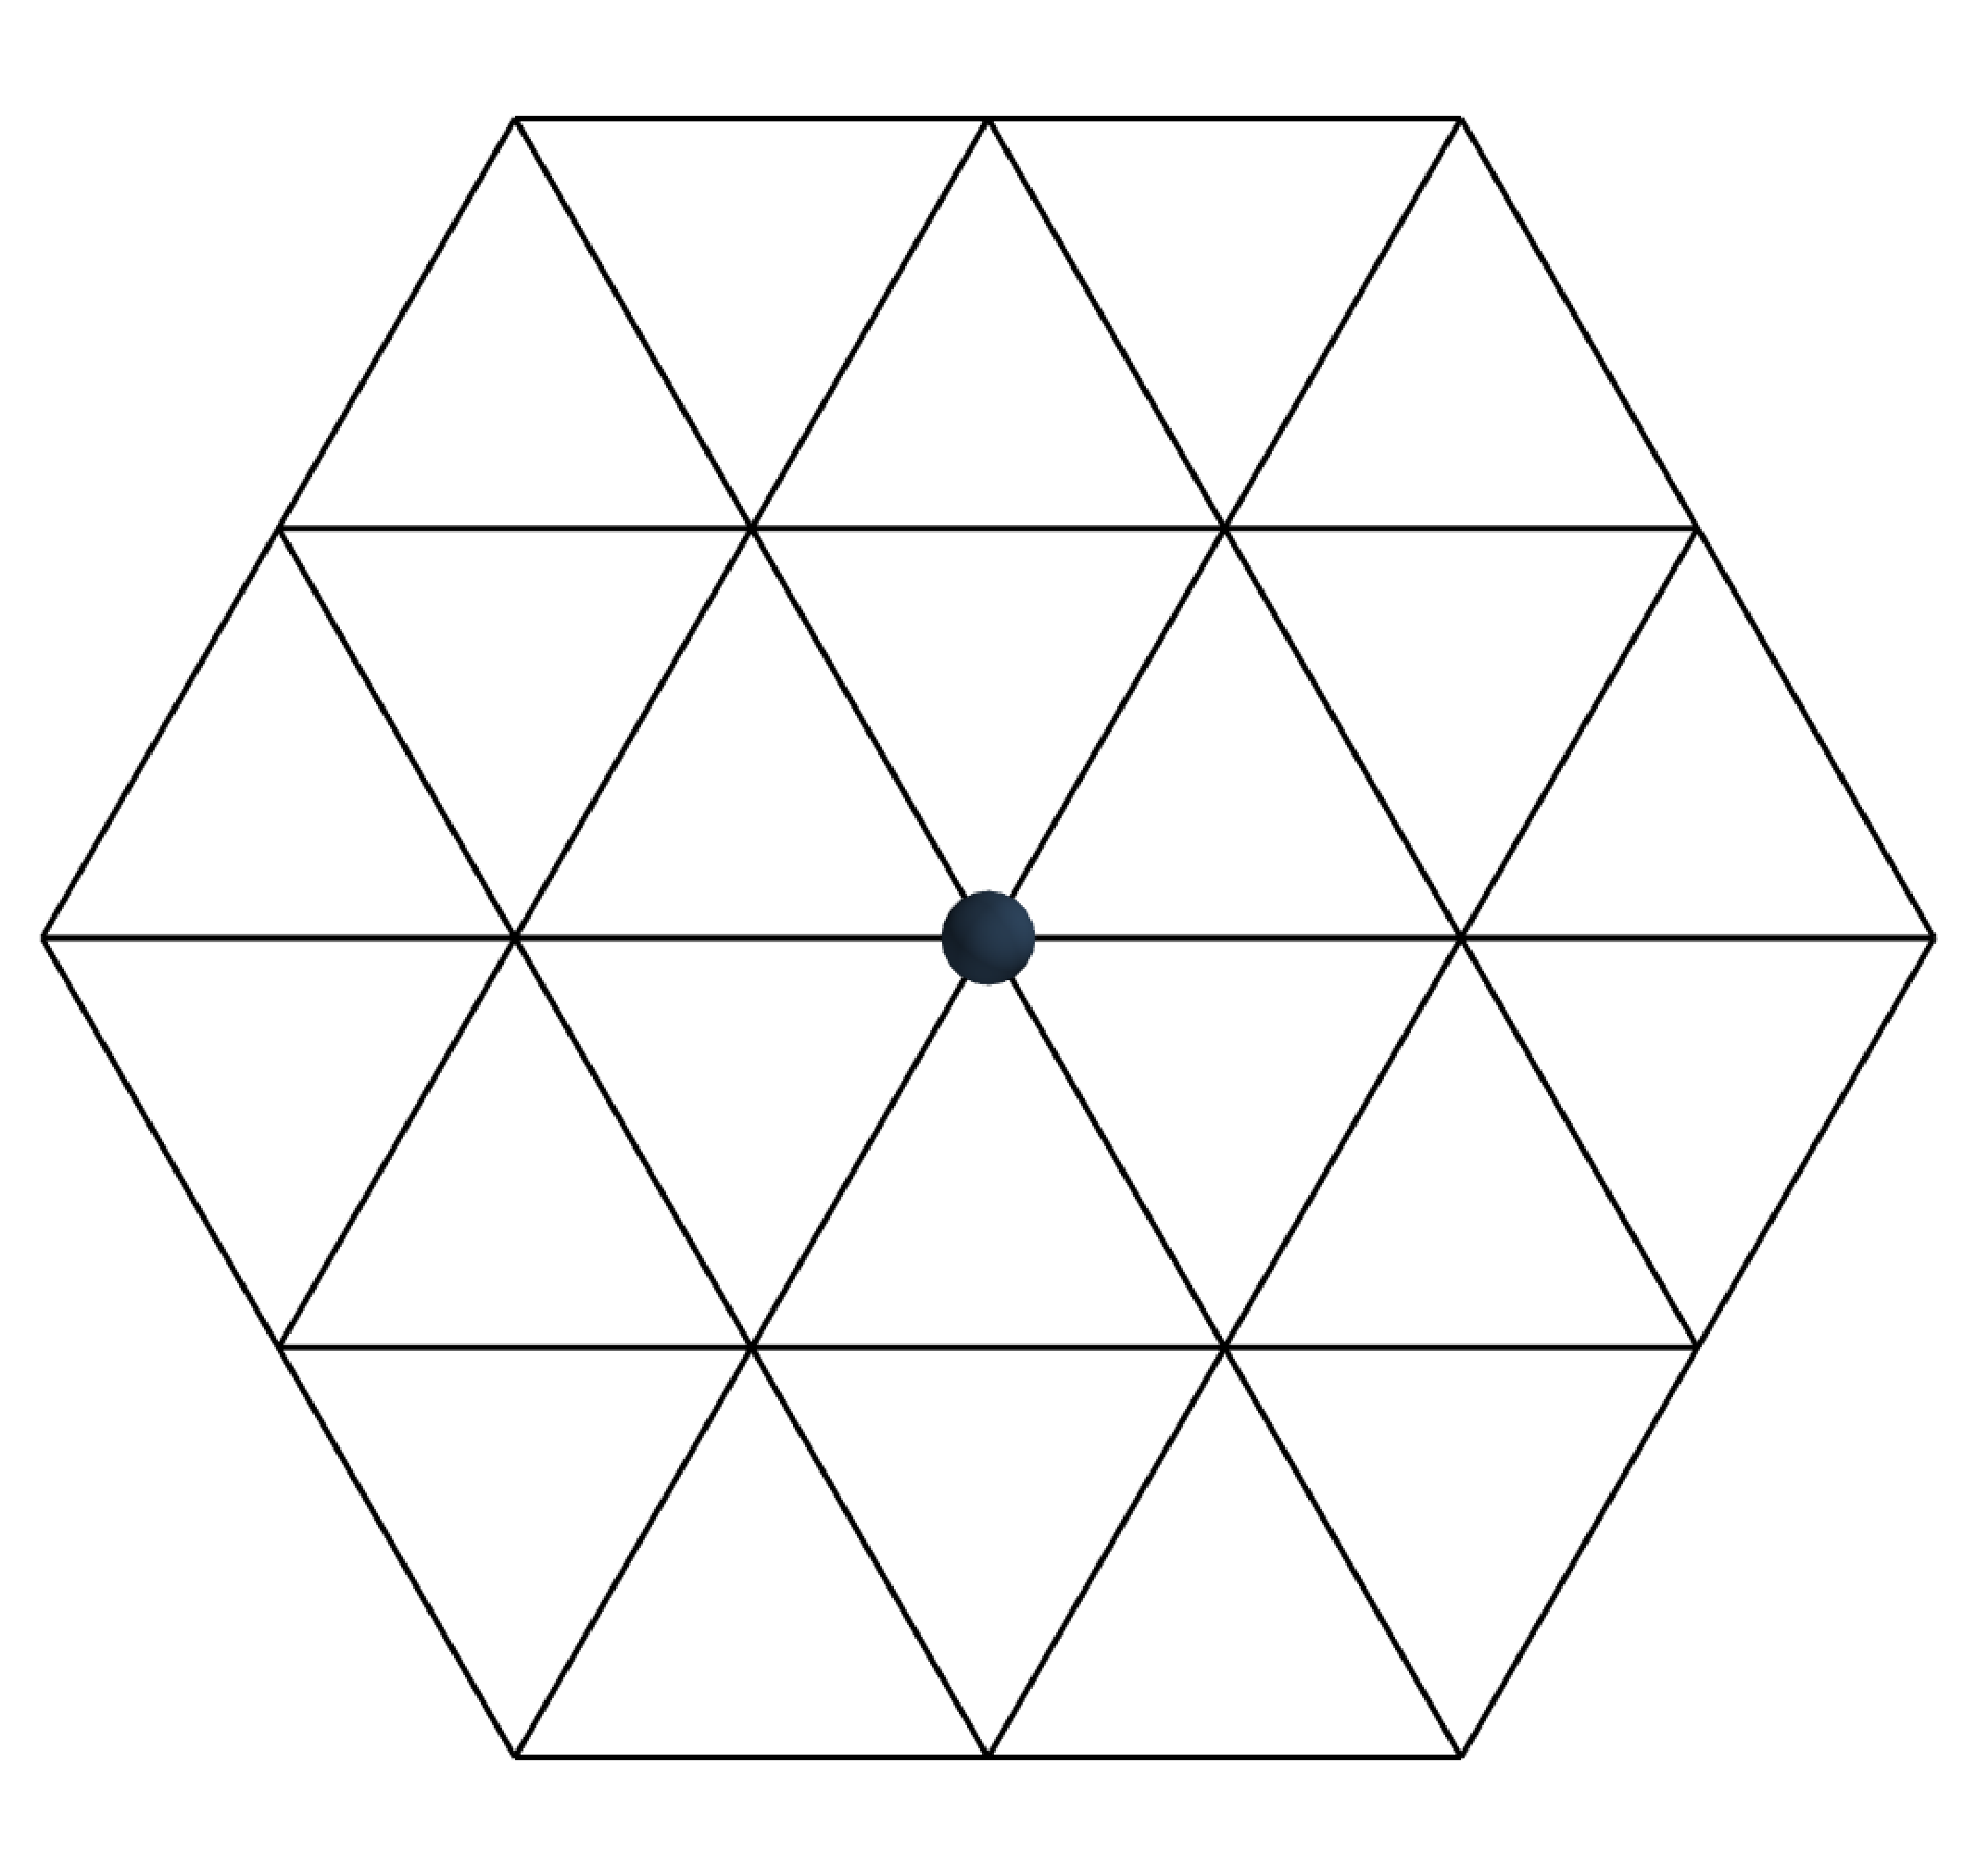
\includegraphics[width=0.25\textwidth]{images/stencils/0_form_simplex.pdf}};
\node[xshift=2pt, yshift=10pt, font=\small, text=black] at (A1.center) {$\simplex{0}{\l}{\coarseIdxone}$};

\node (B1) at (\xB, \yOne)
    {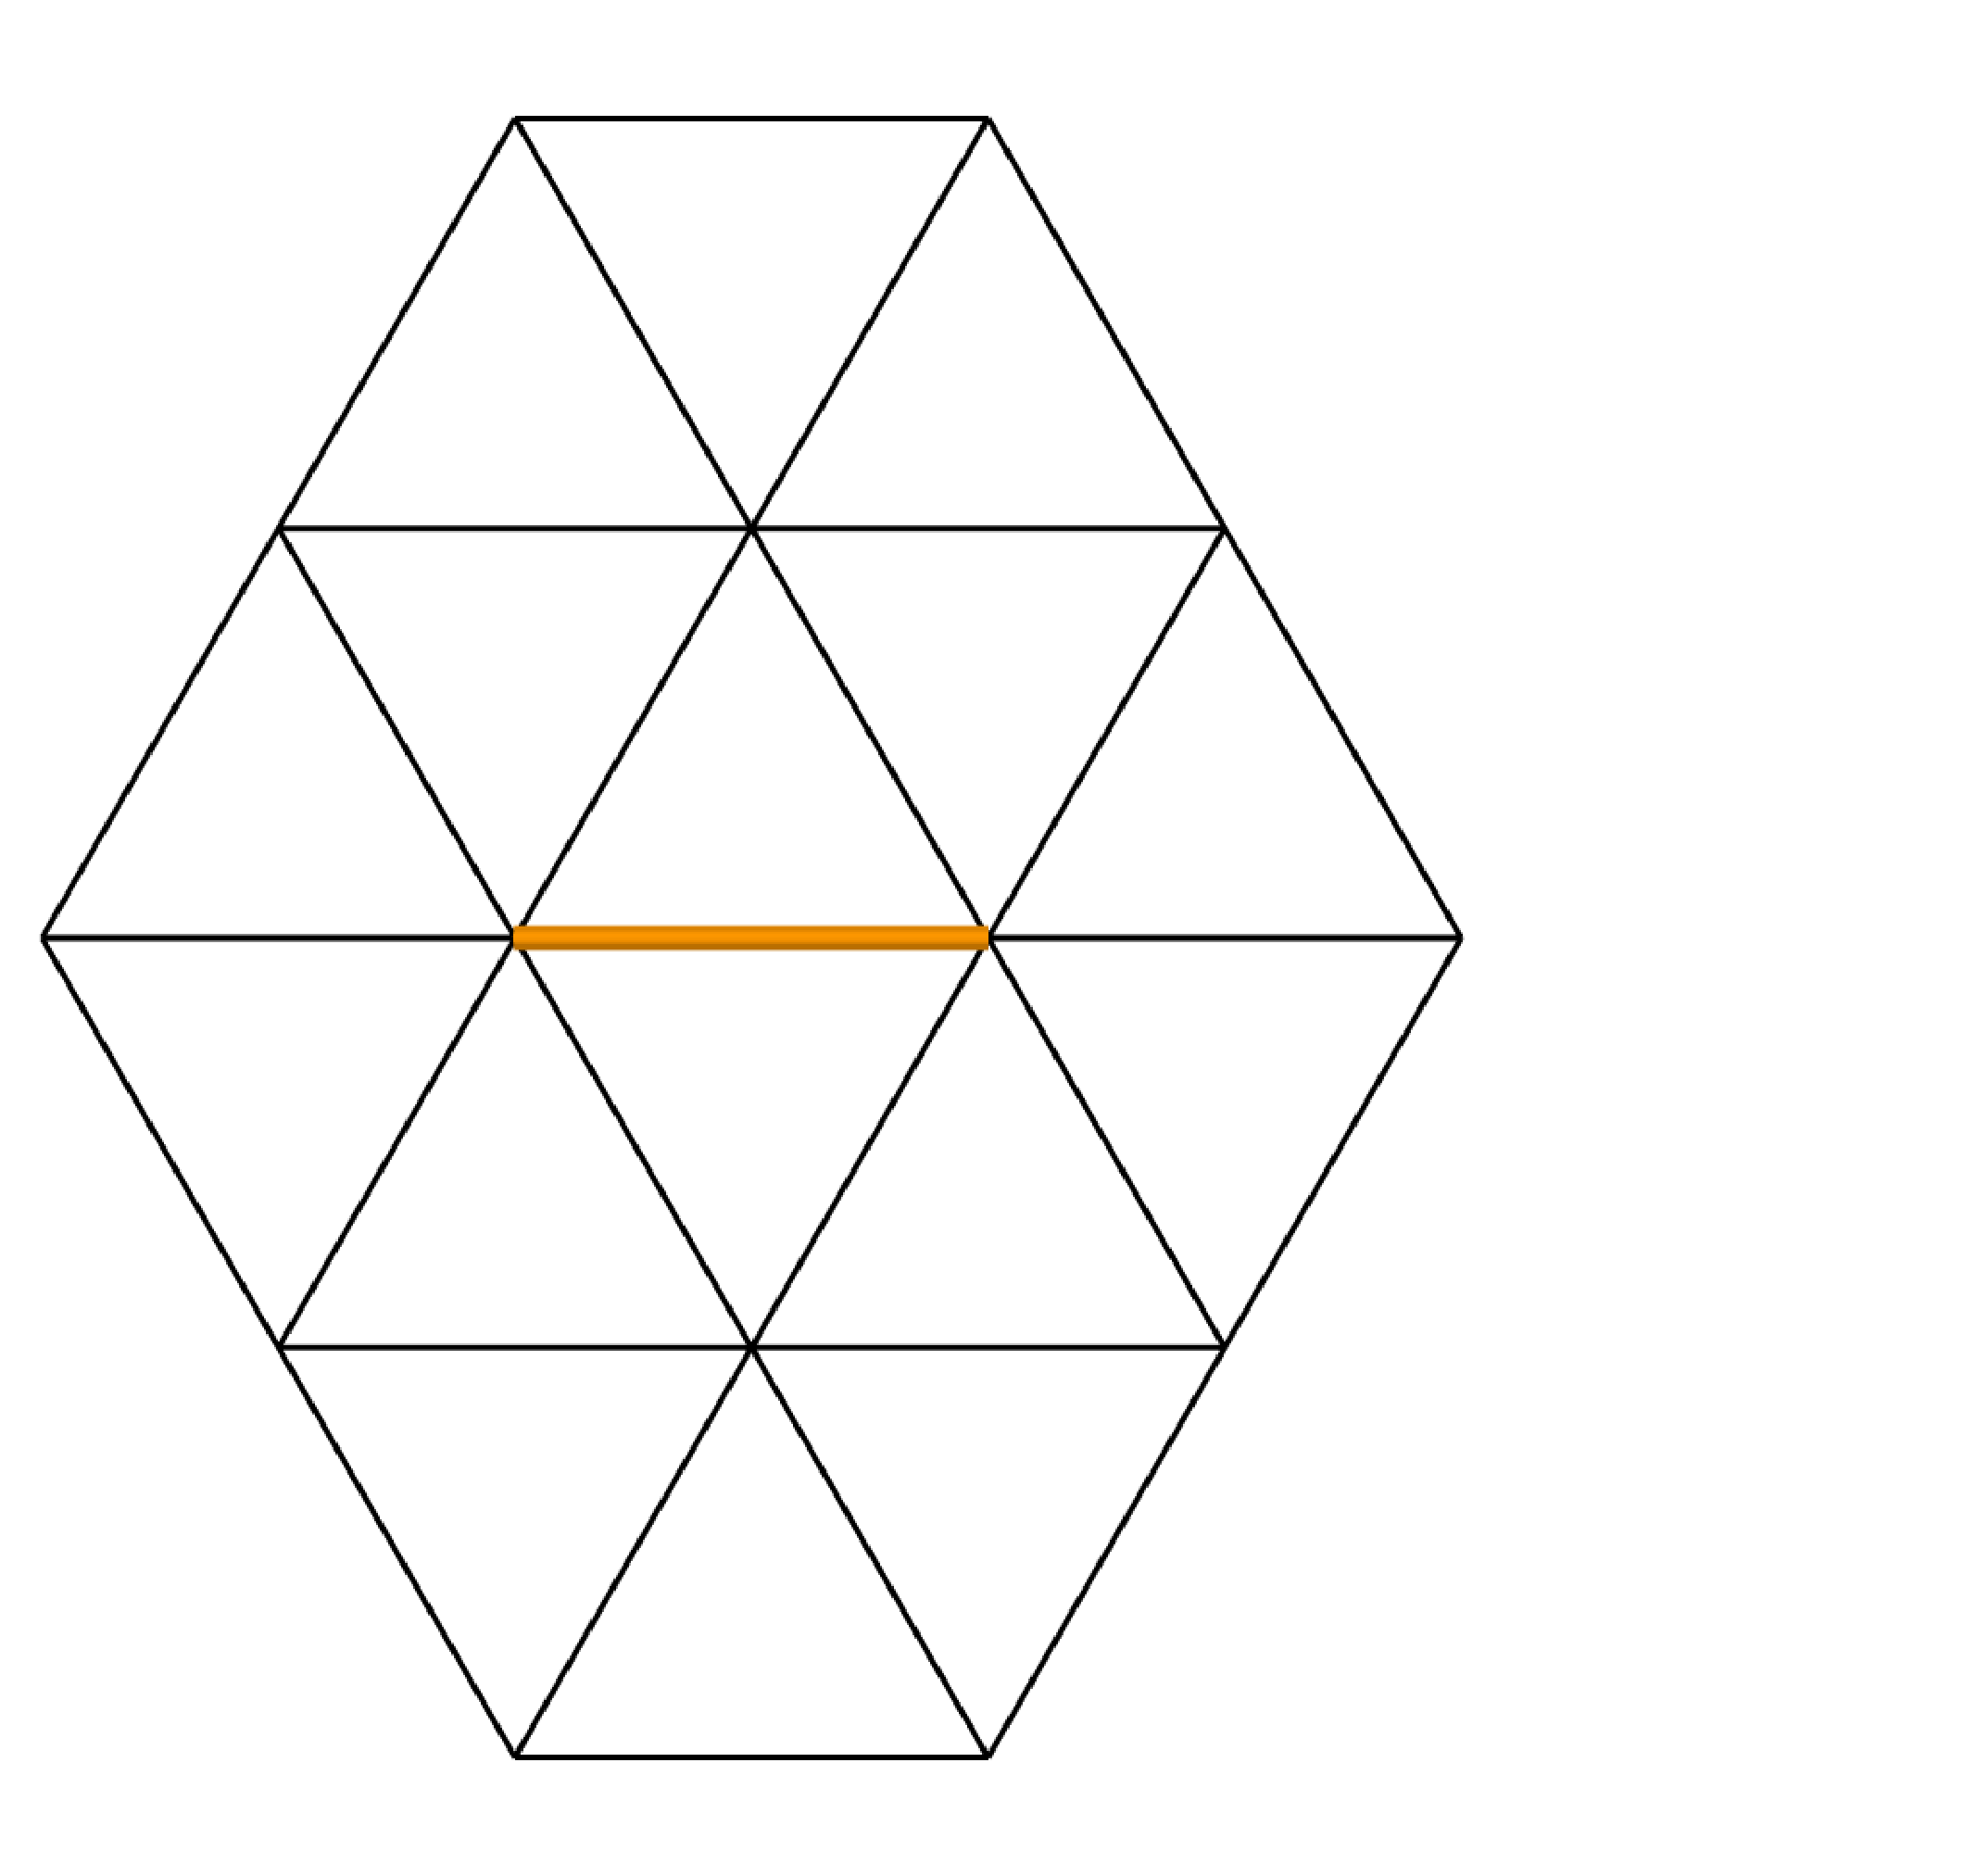
\includegraphics[width=0.25\textwidth, trim=10pt 0pt 10pt 0pt, clip]{images/stencils/1_form_simplex.pdf}};
\node[xshift=-12pt, yshift=10pt, font=\small, text=black] at (B1.center) {$\simplex{1}{\l}{\coarseIdxone}$};

\node (C1) at (\xC, \yOne)
    {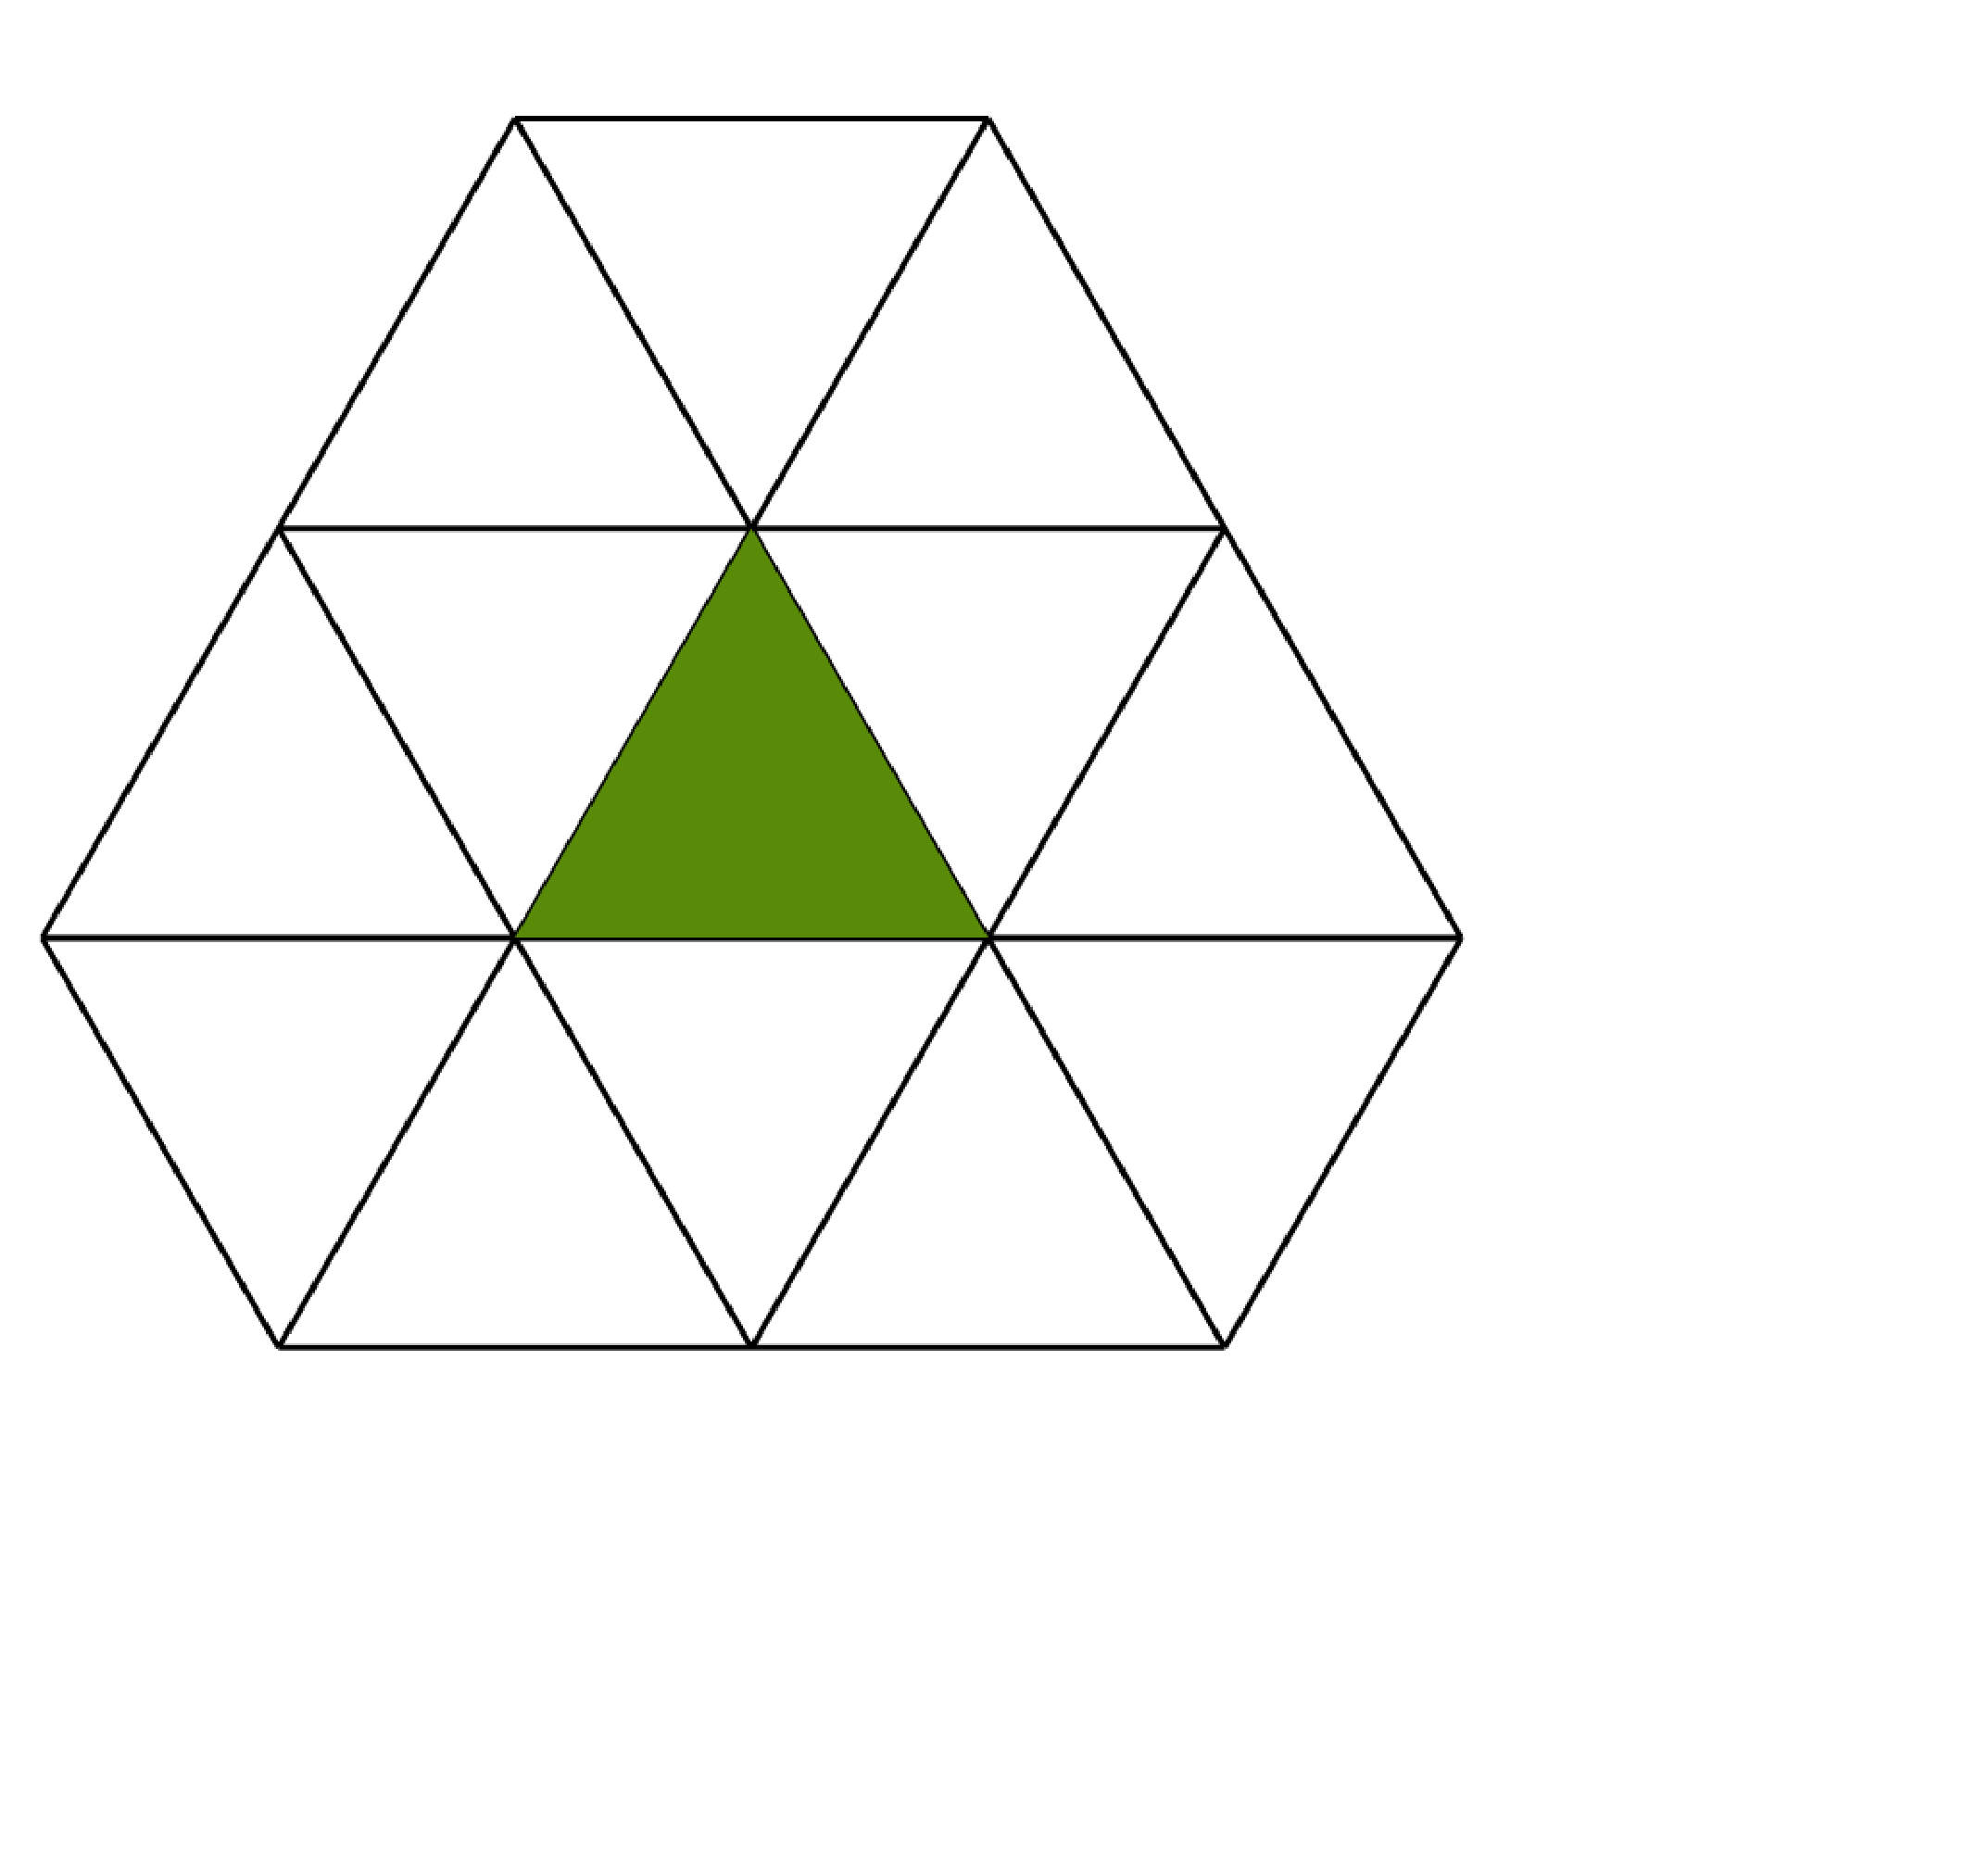
\includegraphics[width=0.25\textwidth]{images/stencils/2_form_simplex.pdf}};
\node[xshift=-12pt, yshift=8pt, font=\small, text=black] at (C1.center) {$\simplex{2}{\l}{\coarseIdxone}$};

\node (A2) at (\xA, \yTwo)
    {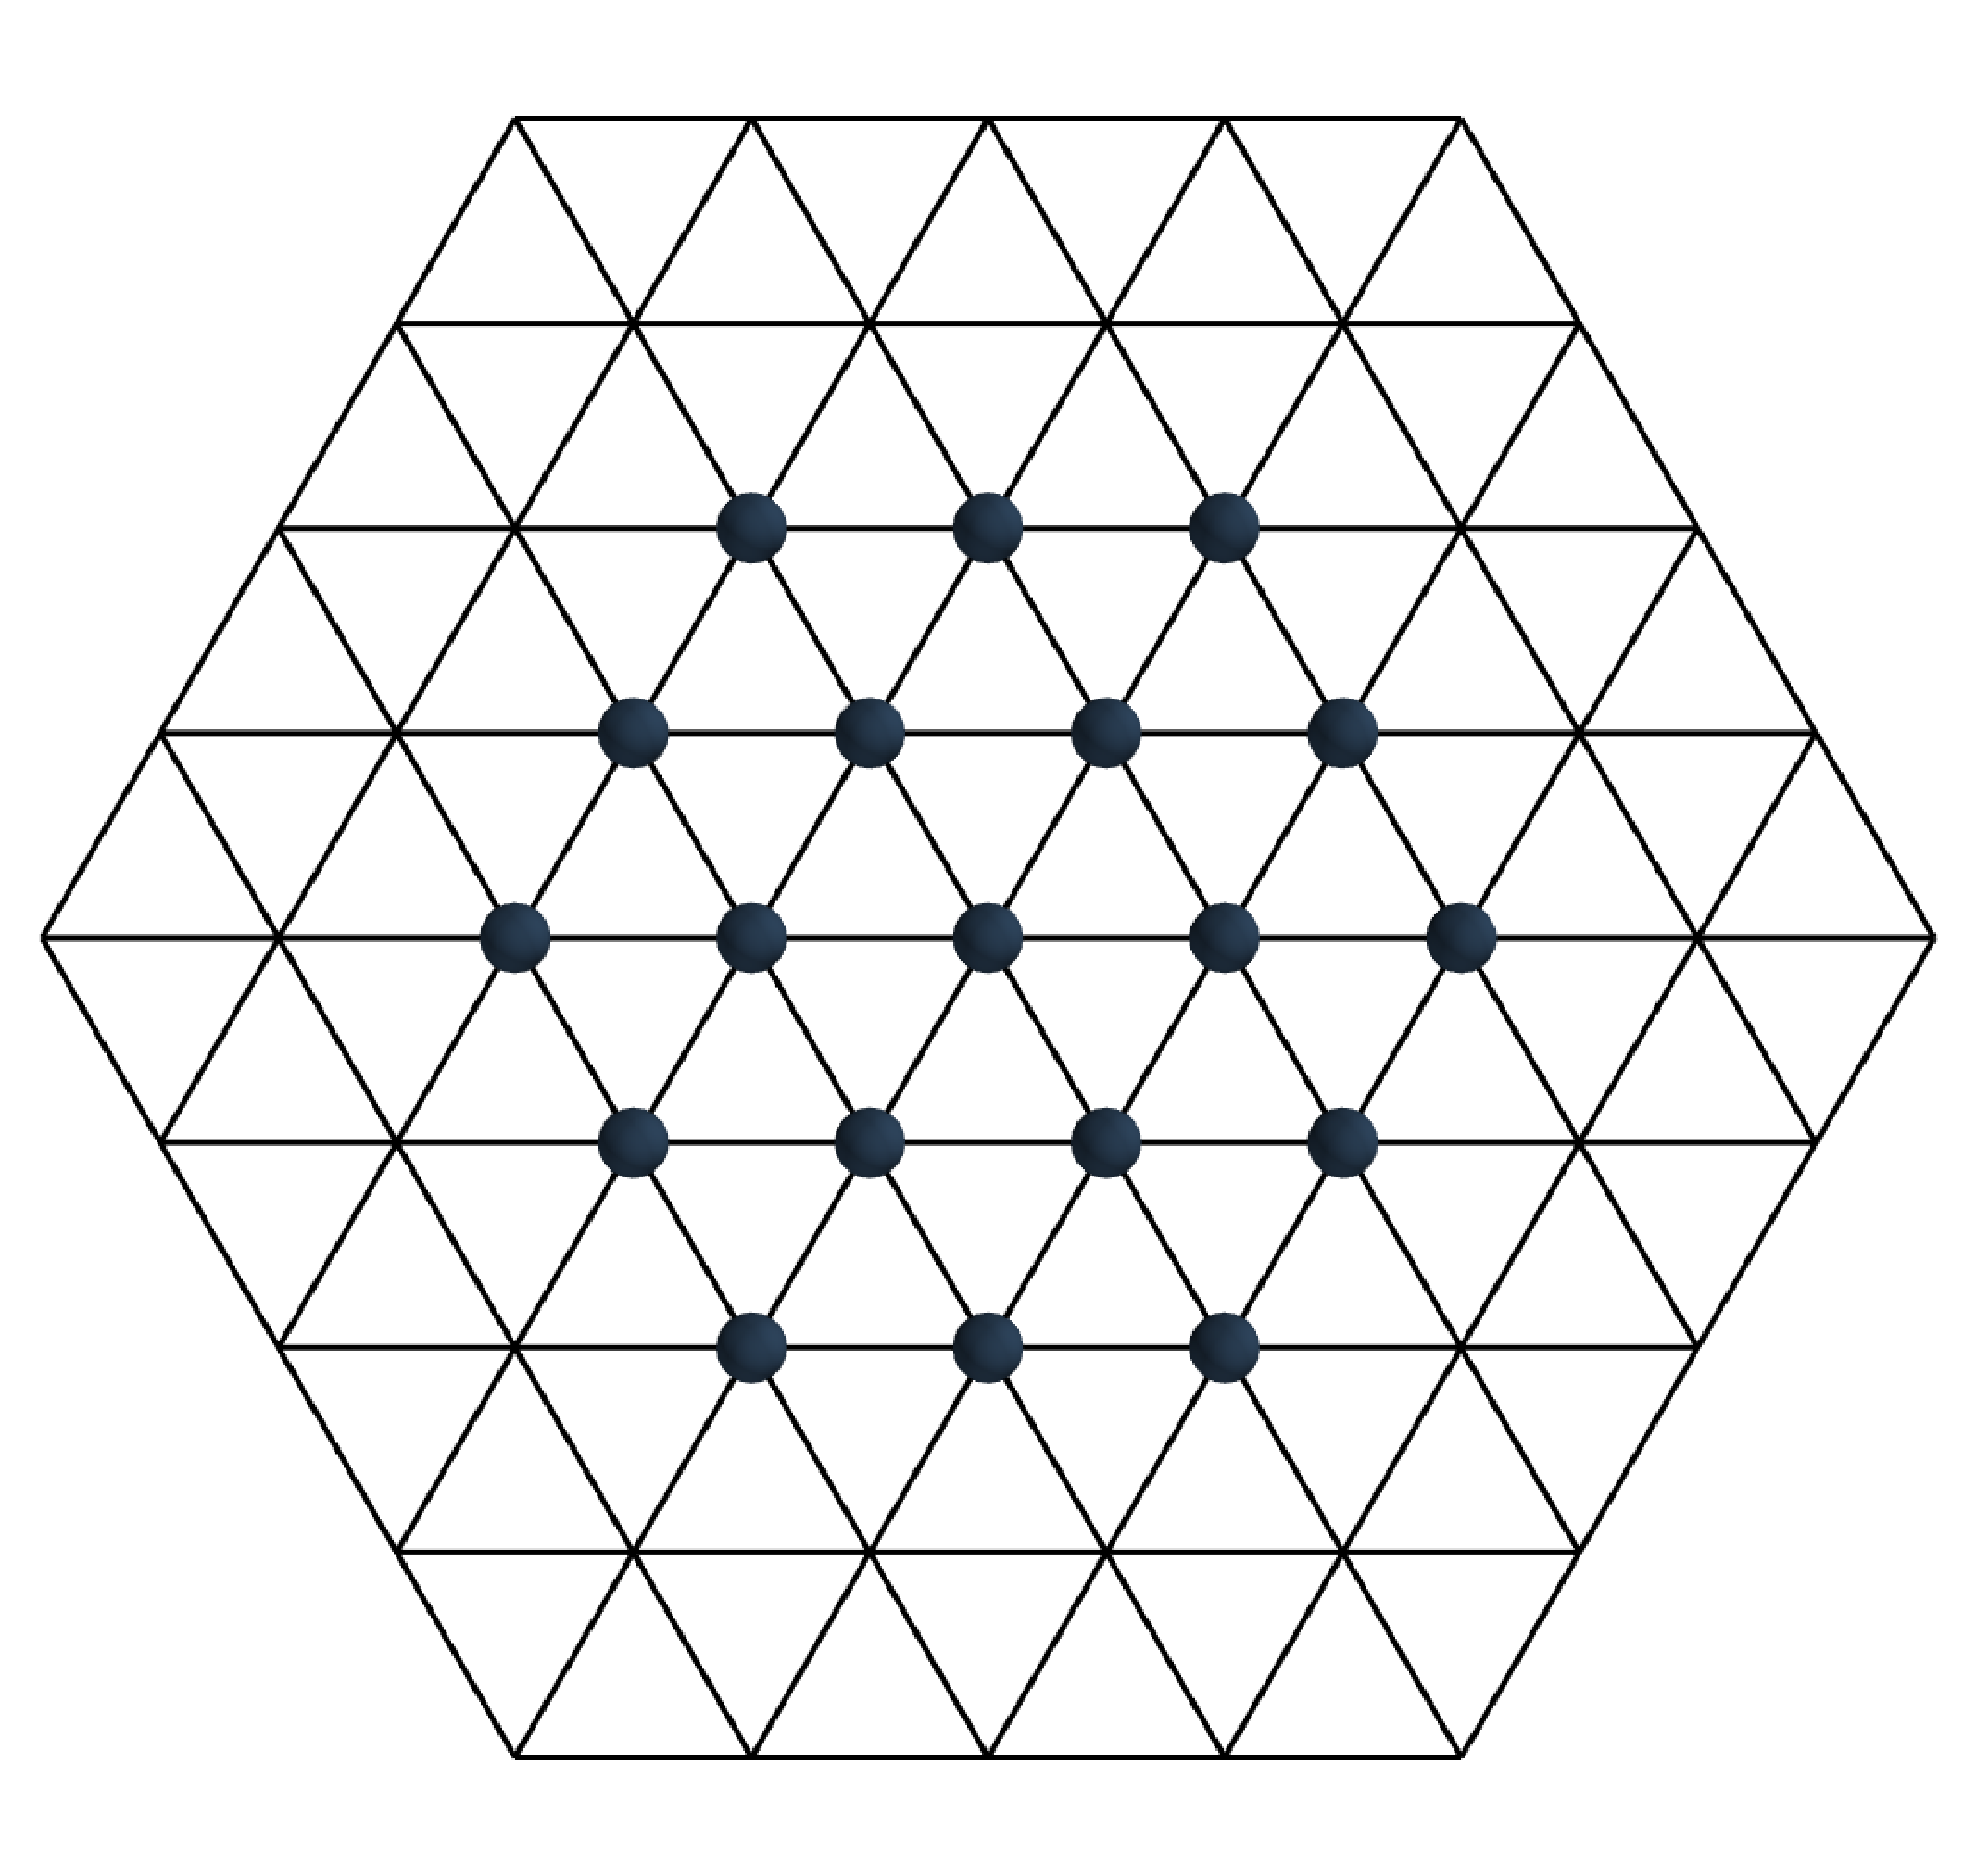
\includegraphics[width=0.25\textwidth]{images/stencils/0_form_refinement_stencil.pdf}};

\node (B2) at (\xB, \yTwo)
    {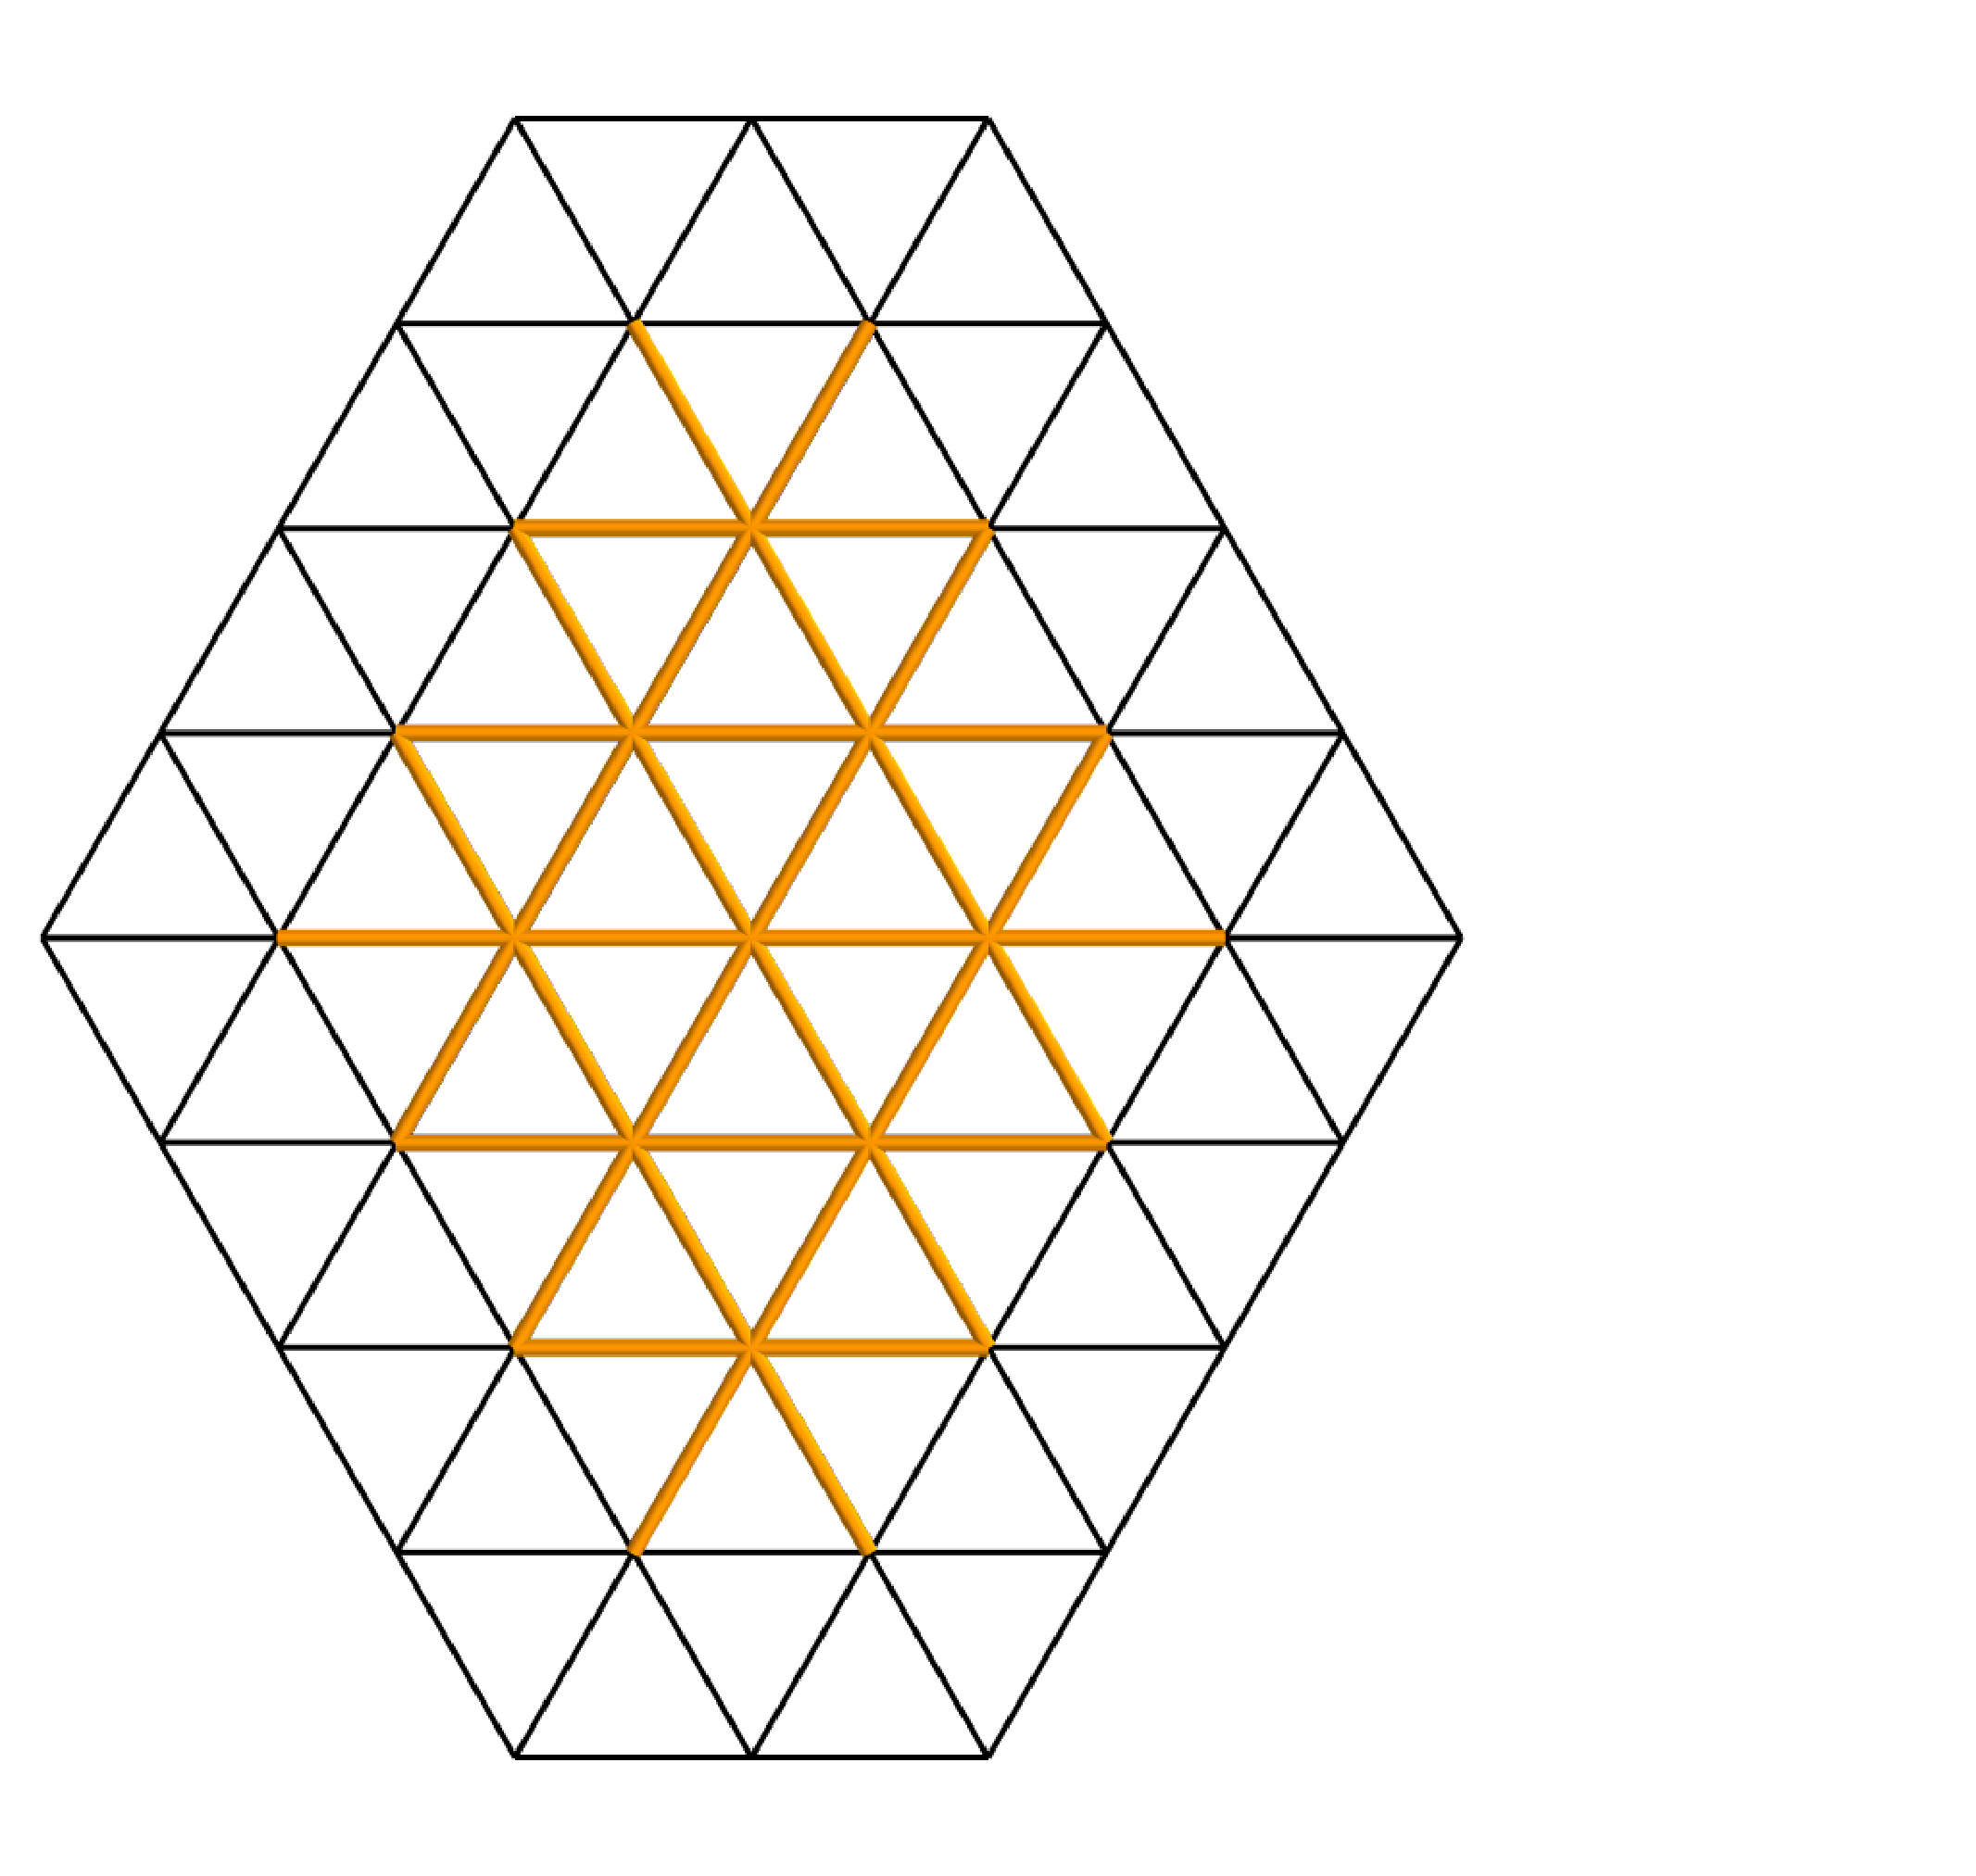
\includegraphics[width=0.25\textwidth, trim=10pt 0pt 10pt 0pt, clip]{images/stencils/1_form_refinement_stencil.pdf}};

\node (C2) at (\xC, \yTwo)
    {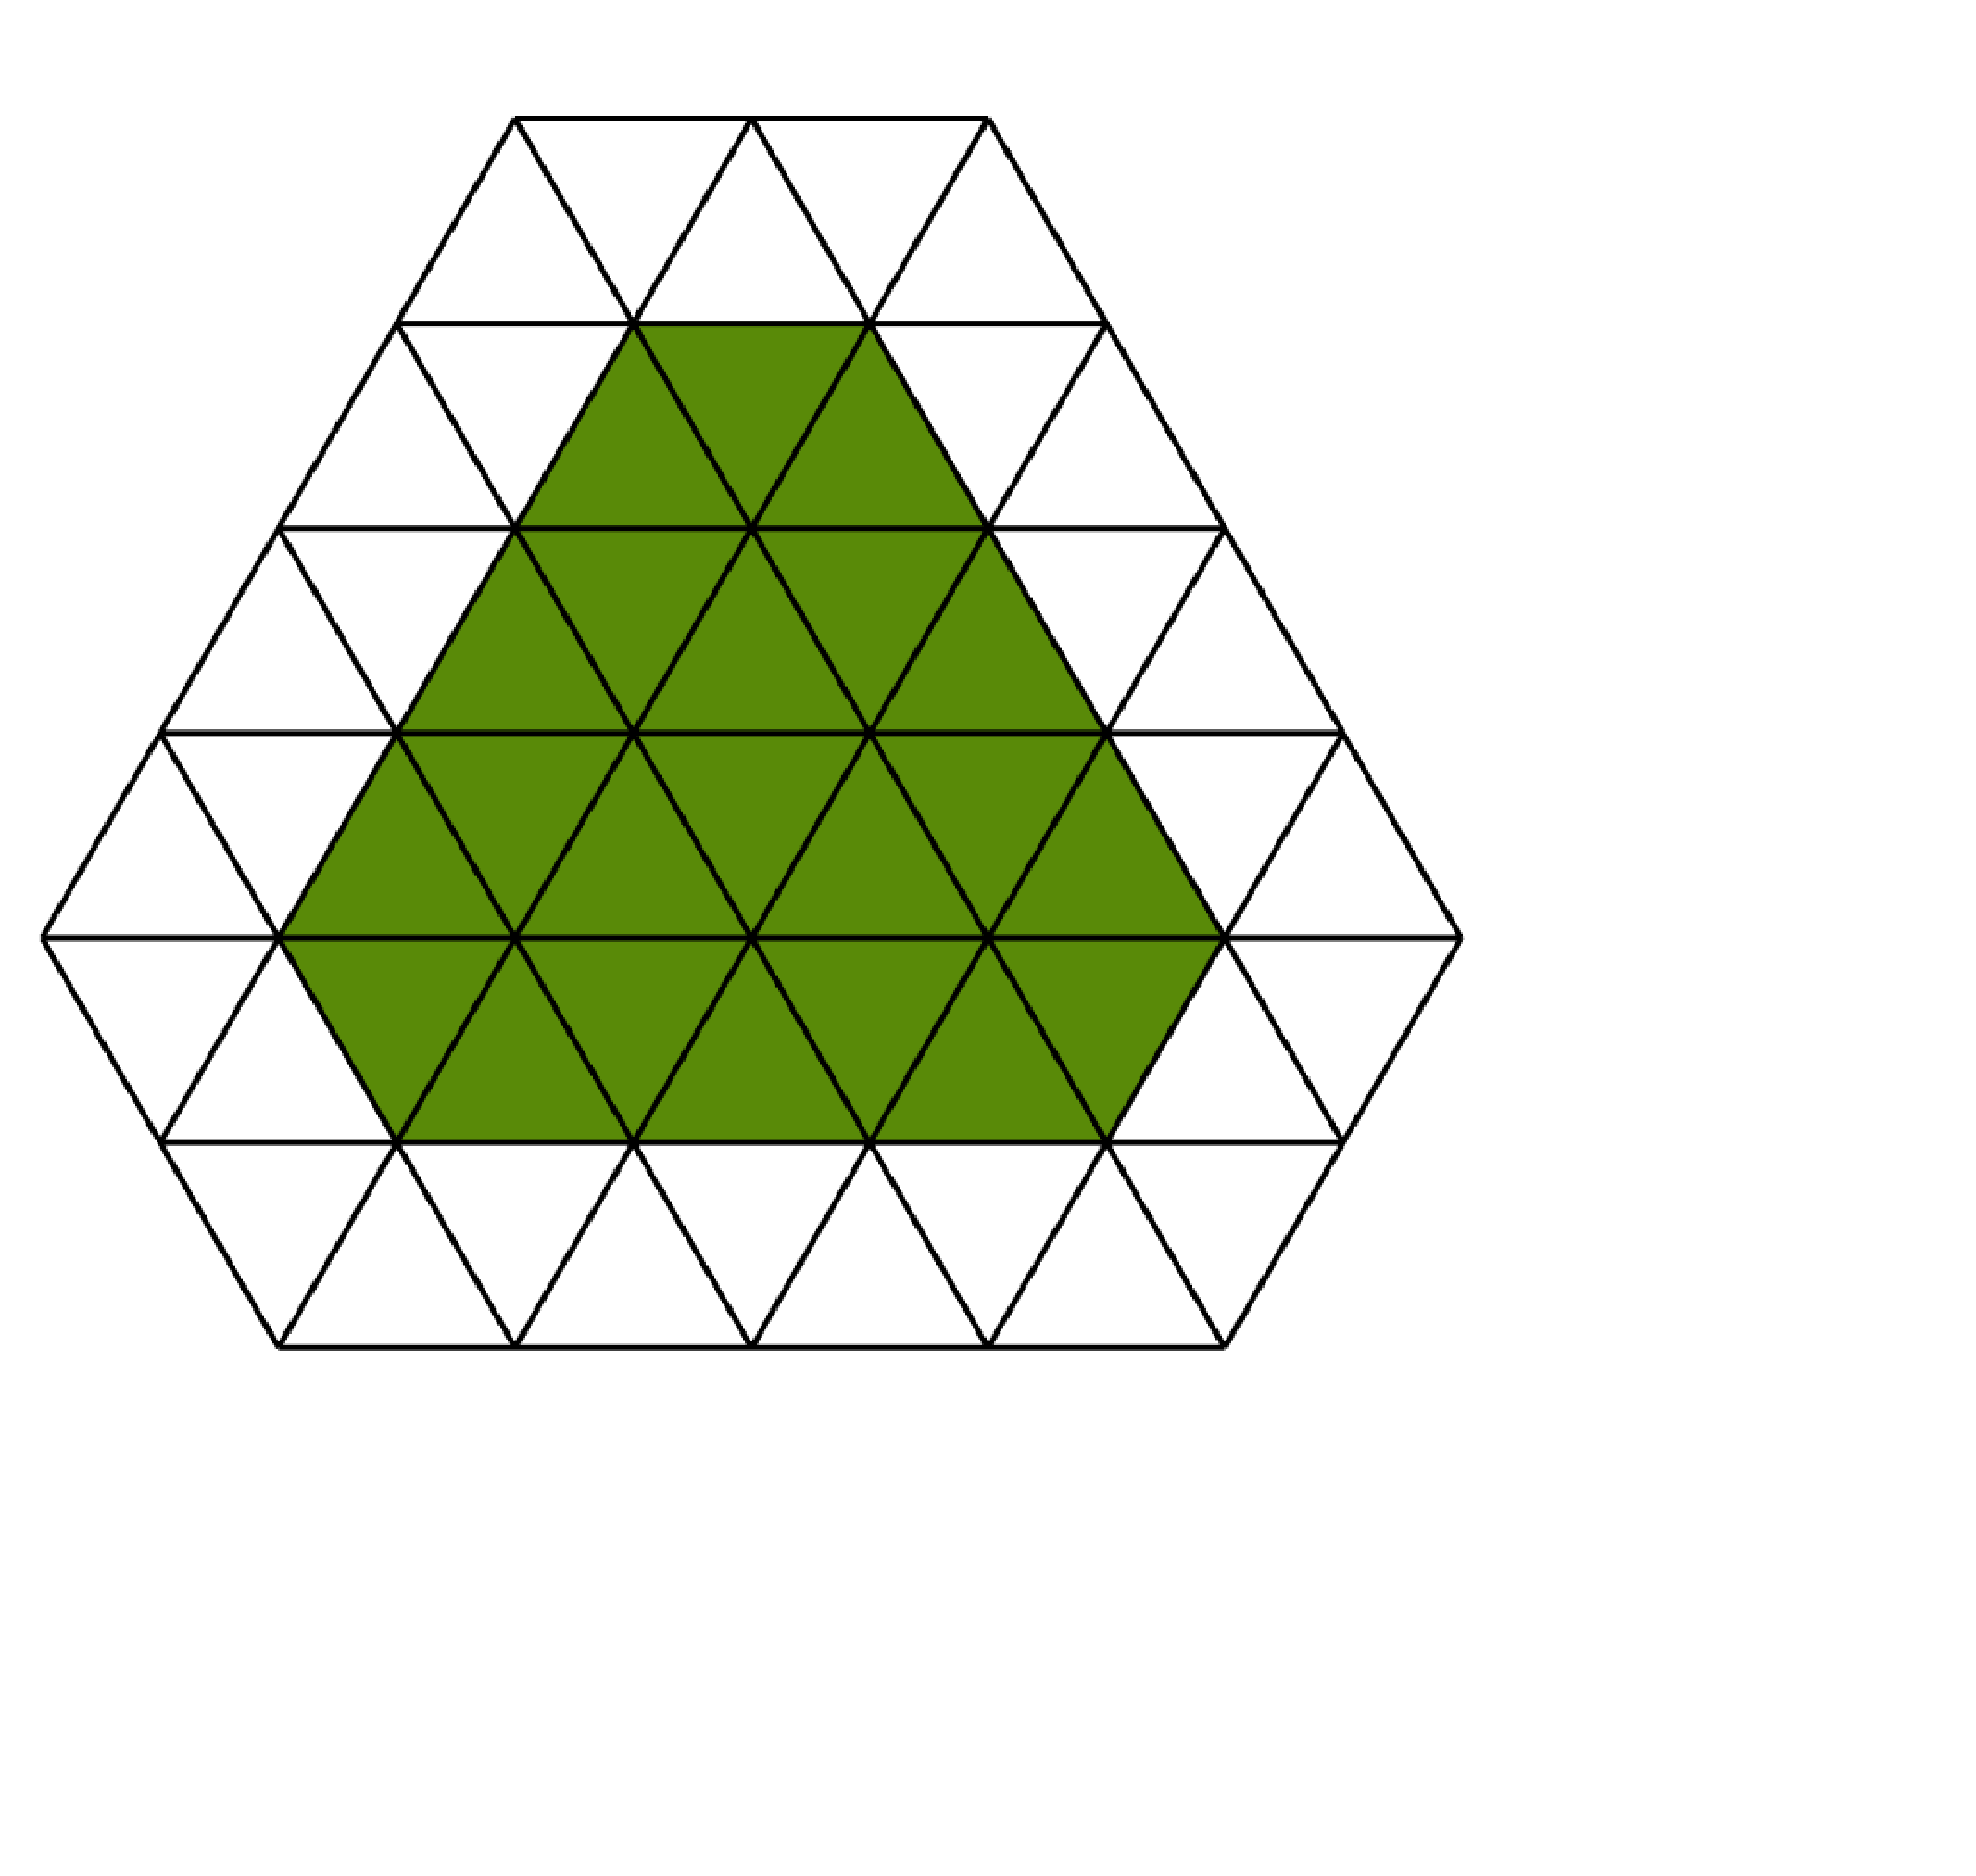
\includegraphics[width=0.25\textwidth]{images/stencils/2_form_refinement_stencil.pdf}};

\draw[arr] (A1.south) -- (A2.north) node[midway, right, font=\small] {$\;\; \cRSt\big( \simplex{0}{\l}{\coarseIdxone} \big)$};
\draw[arr] ([xshift=-14pt]B1.south) -- ([xshift=-14pt]B2.north) node[midway, right, font=\small] {$\;\; \cRSt\big( \simplex{1}{\l}{\coarseIdxone} \big)$};
\draw[arr] ([xshift=-14pt]C1.south) -- ([xshift=-14pt]C2.north) node[midway, right, font=\small] {$\;\; \cRSt\big( \simplex{2}{\l}{\coarseIdxone} \big)$};

\end{tikzpicture}
\end{center}
\vspace{-5mm}
\caption{Refinement stencils of $0$-, $1$- and $2$-form basis functions.}
\end{figure}

\FloatBarrier

\subsection{Derivative Stencil}

The derivative stencil describes the $k+1$-form basis functions needed to re-express the exterior derivative of a $k$-form basis function as a linear combination. It represents a tool that is helpful to select active DoFs and ensure that the spaces form a differential complex.

\begin{figure}[H]
\begin{center}
\begin{tikzpicture}[
    every node/.style={inner sep=0pt, outer sep=0pt},
    arr/.style={->, >=Stealth, line width=1.5pt, shorten >=2pt, shorten <=2pt}
]

\def\xA{0cm}
\def\xB{5cm}
\def\yOne{0cm}
\def\yTwo{-4.5cm}

\node (A1) at (\xA, \yOne)
    {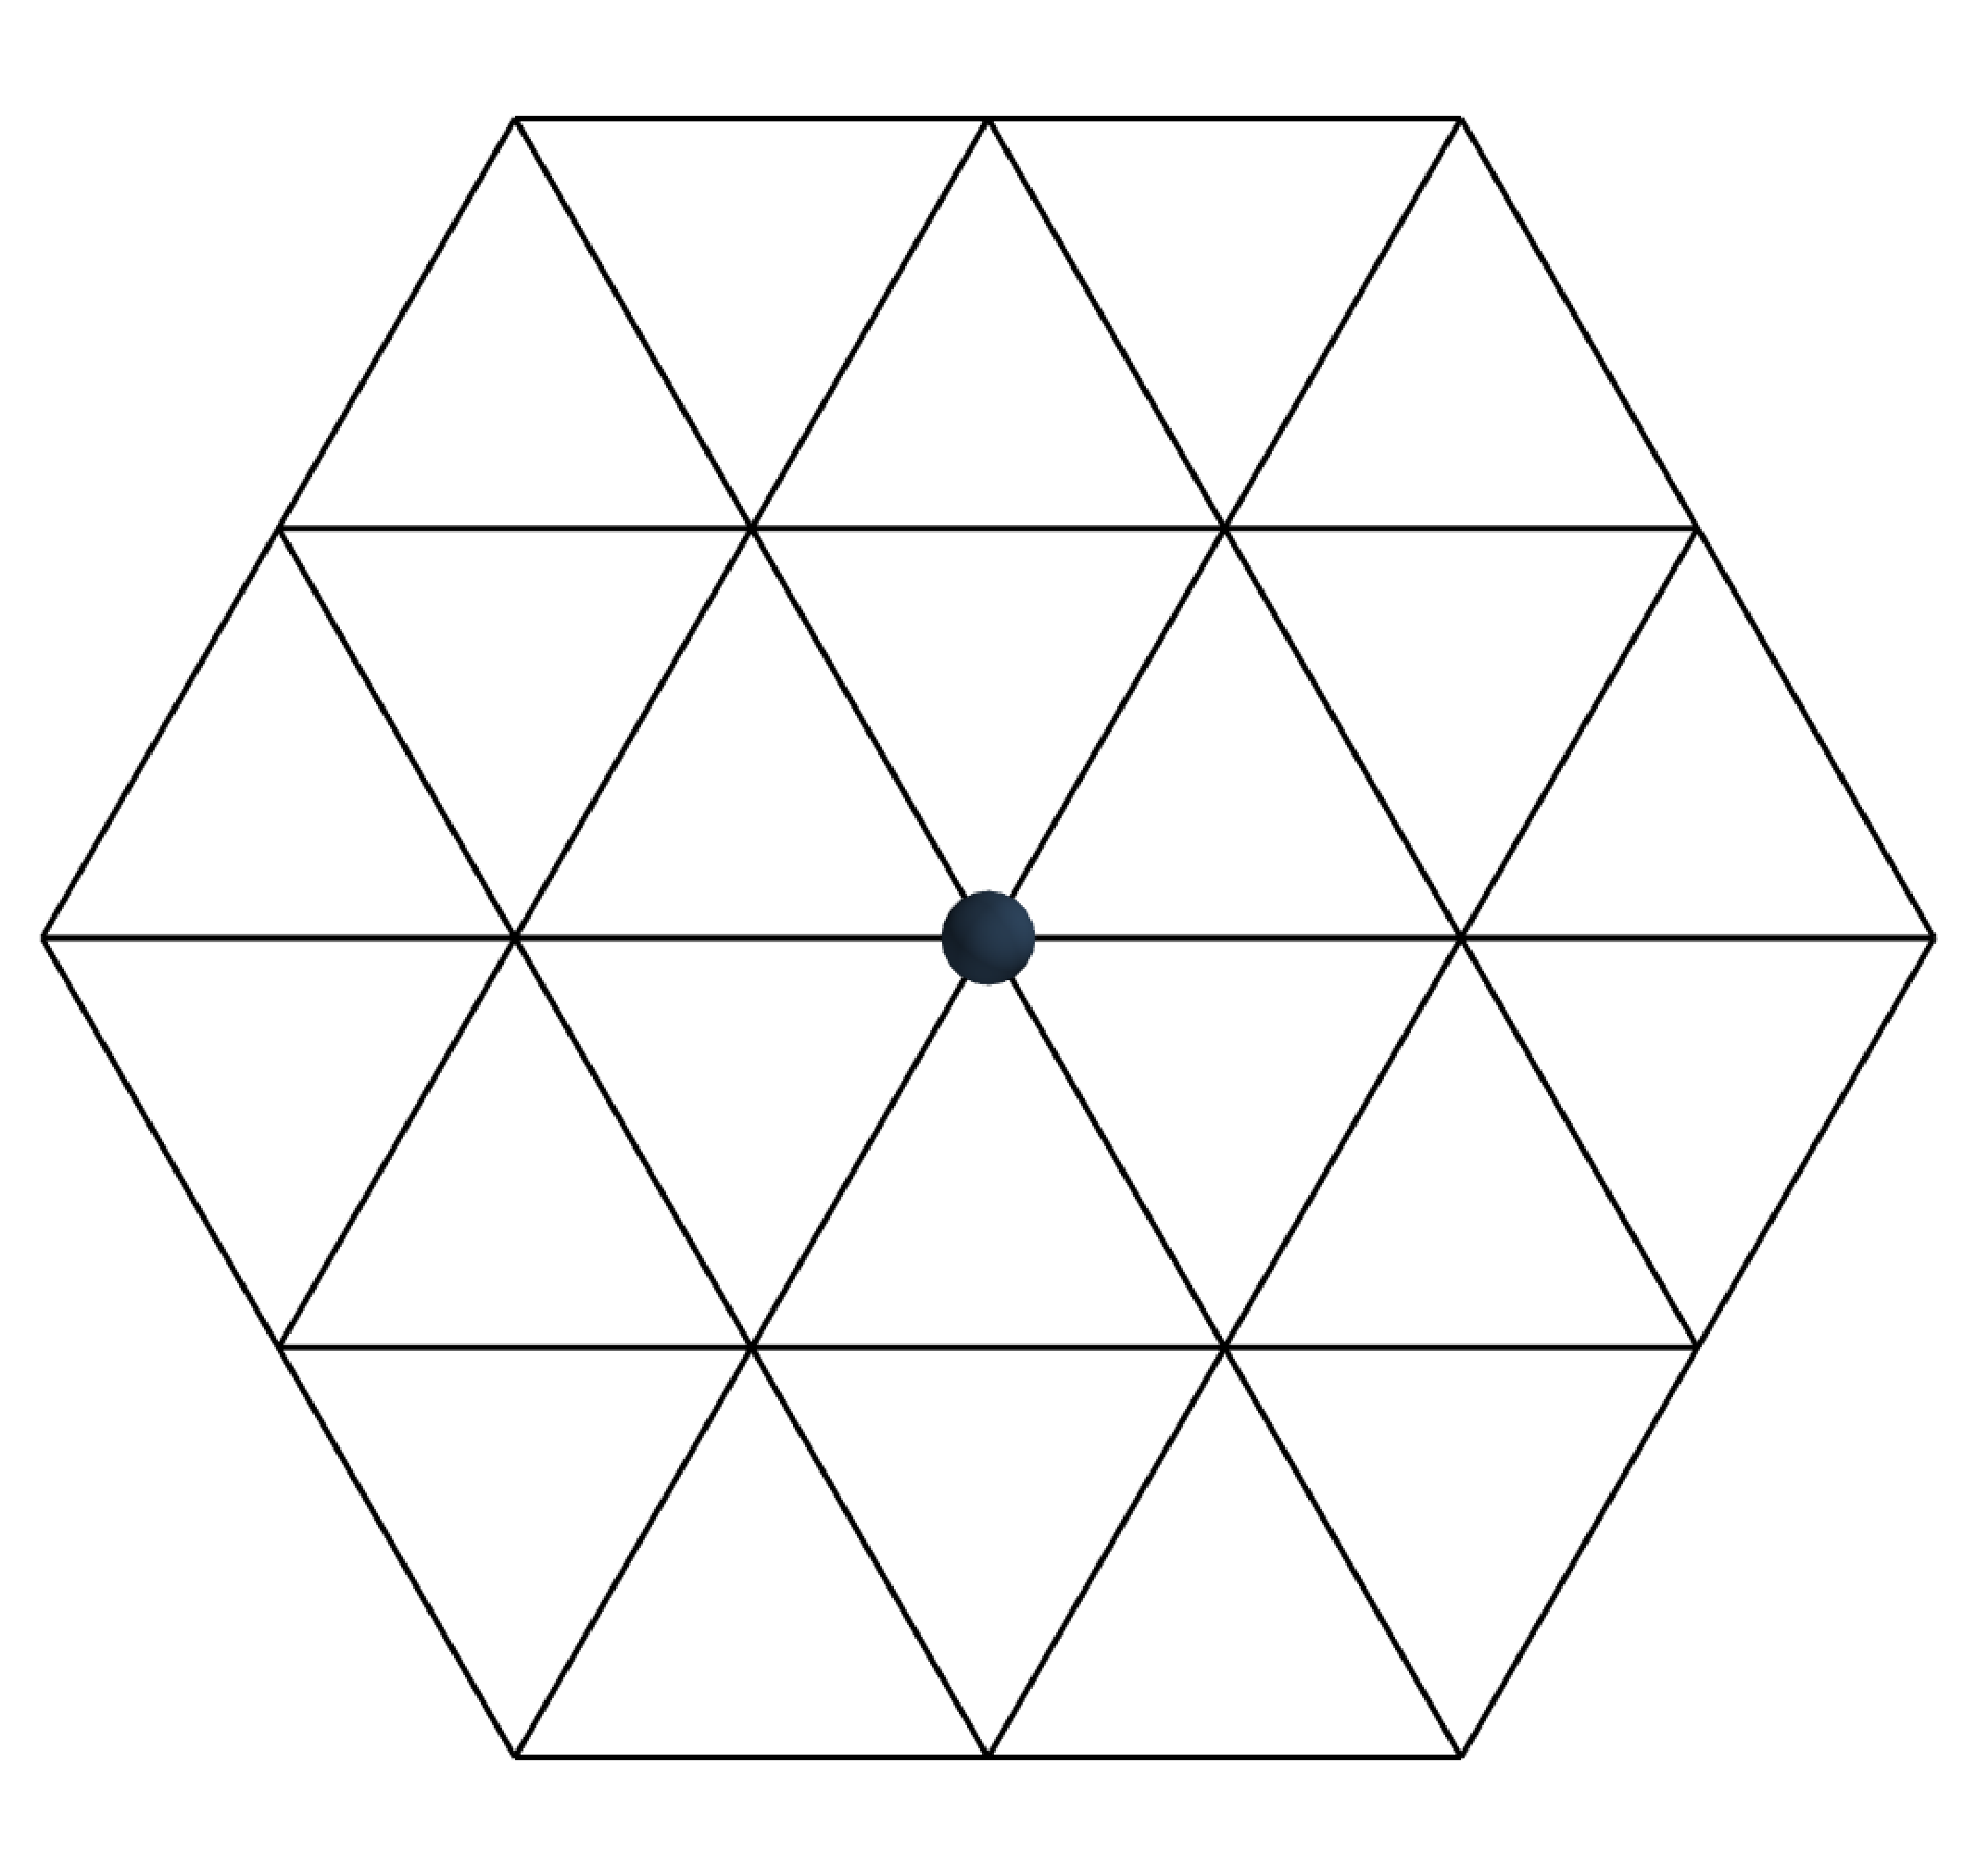
\includegraphics[width=0.25\textwidth]{images/stencils/0_form_simplex.pdf}};
\node[xshift=2pt, yshift=10pt, font=\small, text=black] at (A1.center) {$\simplex{0}{\l}{\coarseIdxone}$};

\node (B1) at (\xB, \yOne)
    {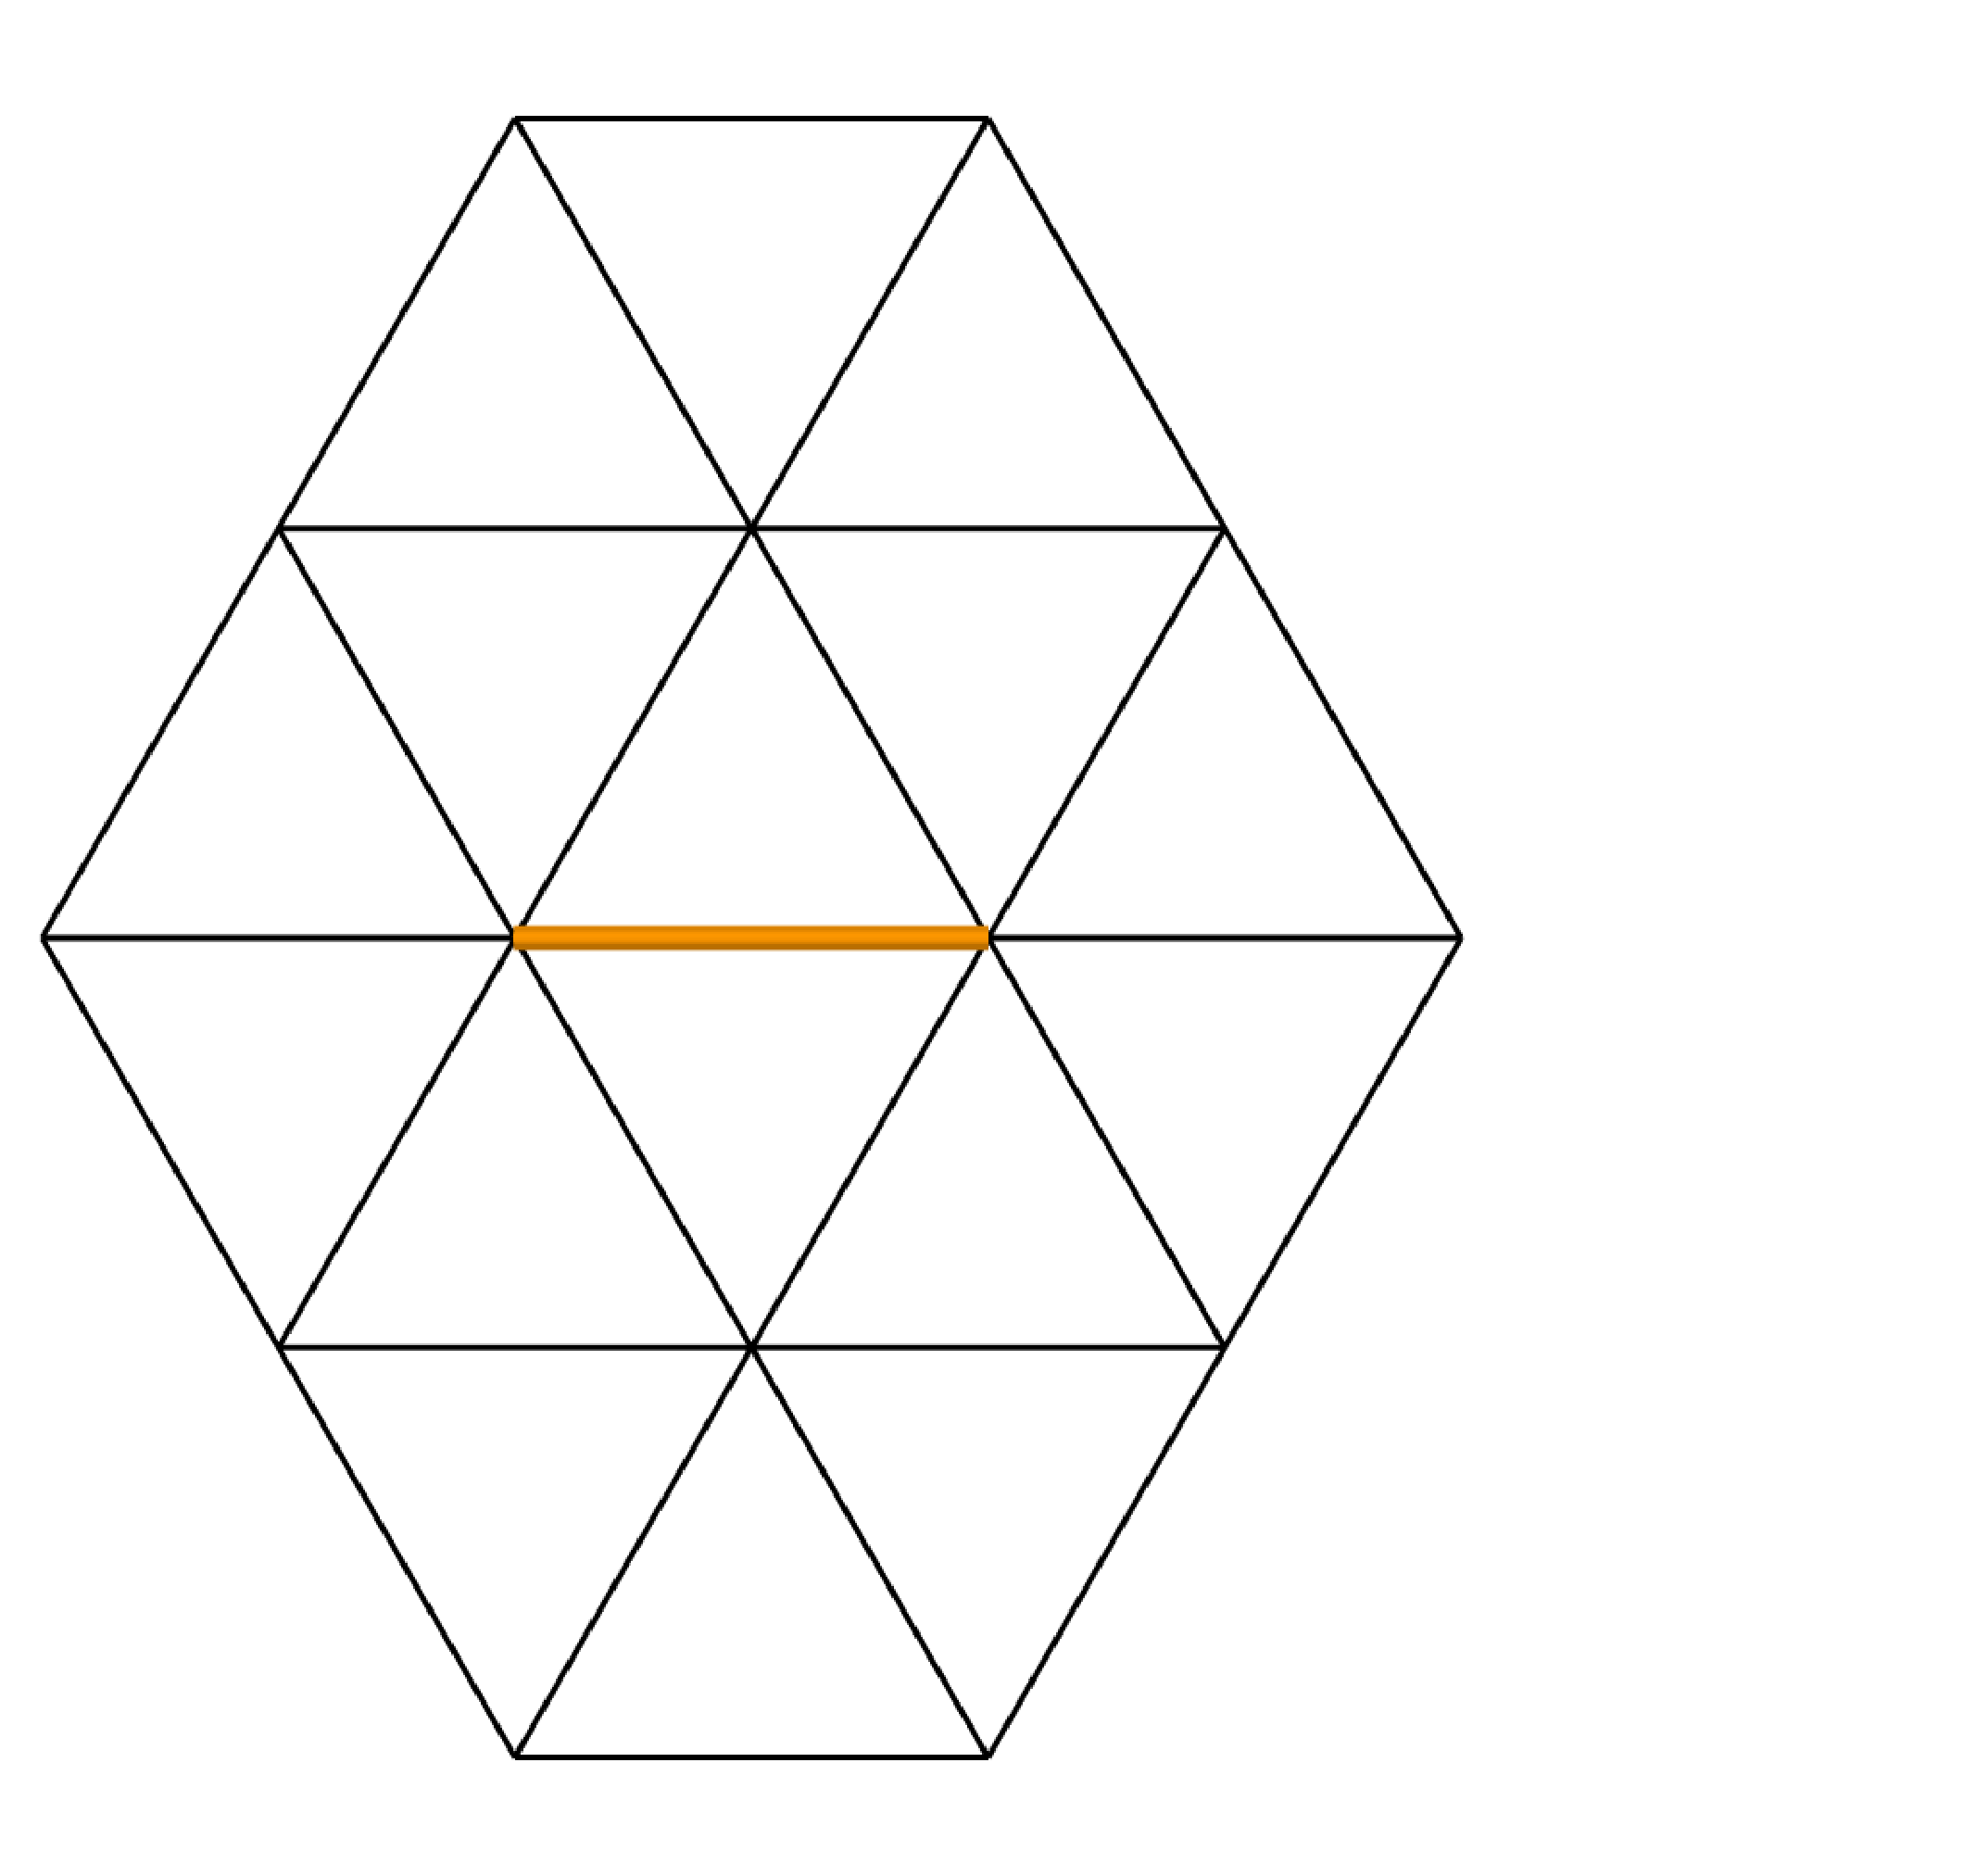
\includegraphics[width=0.25\textwidth, trim=10pt 0pt 10pt 0pt, clip]{images/stencils/1_form_simplex.pdf}};
\node[xshift=-12pt, yshift=10pt, font=\small, text=black] at (B1.center) {$\simplex{1}{\l}{\coarseIdxone}$};

\node (A2) at (\xA, \yTwo)
    {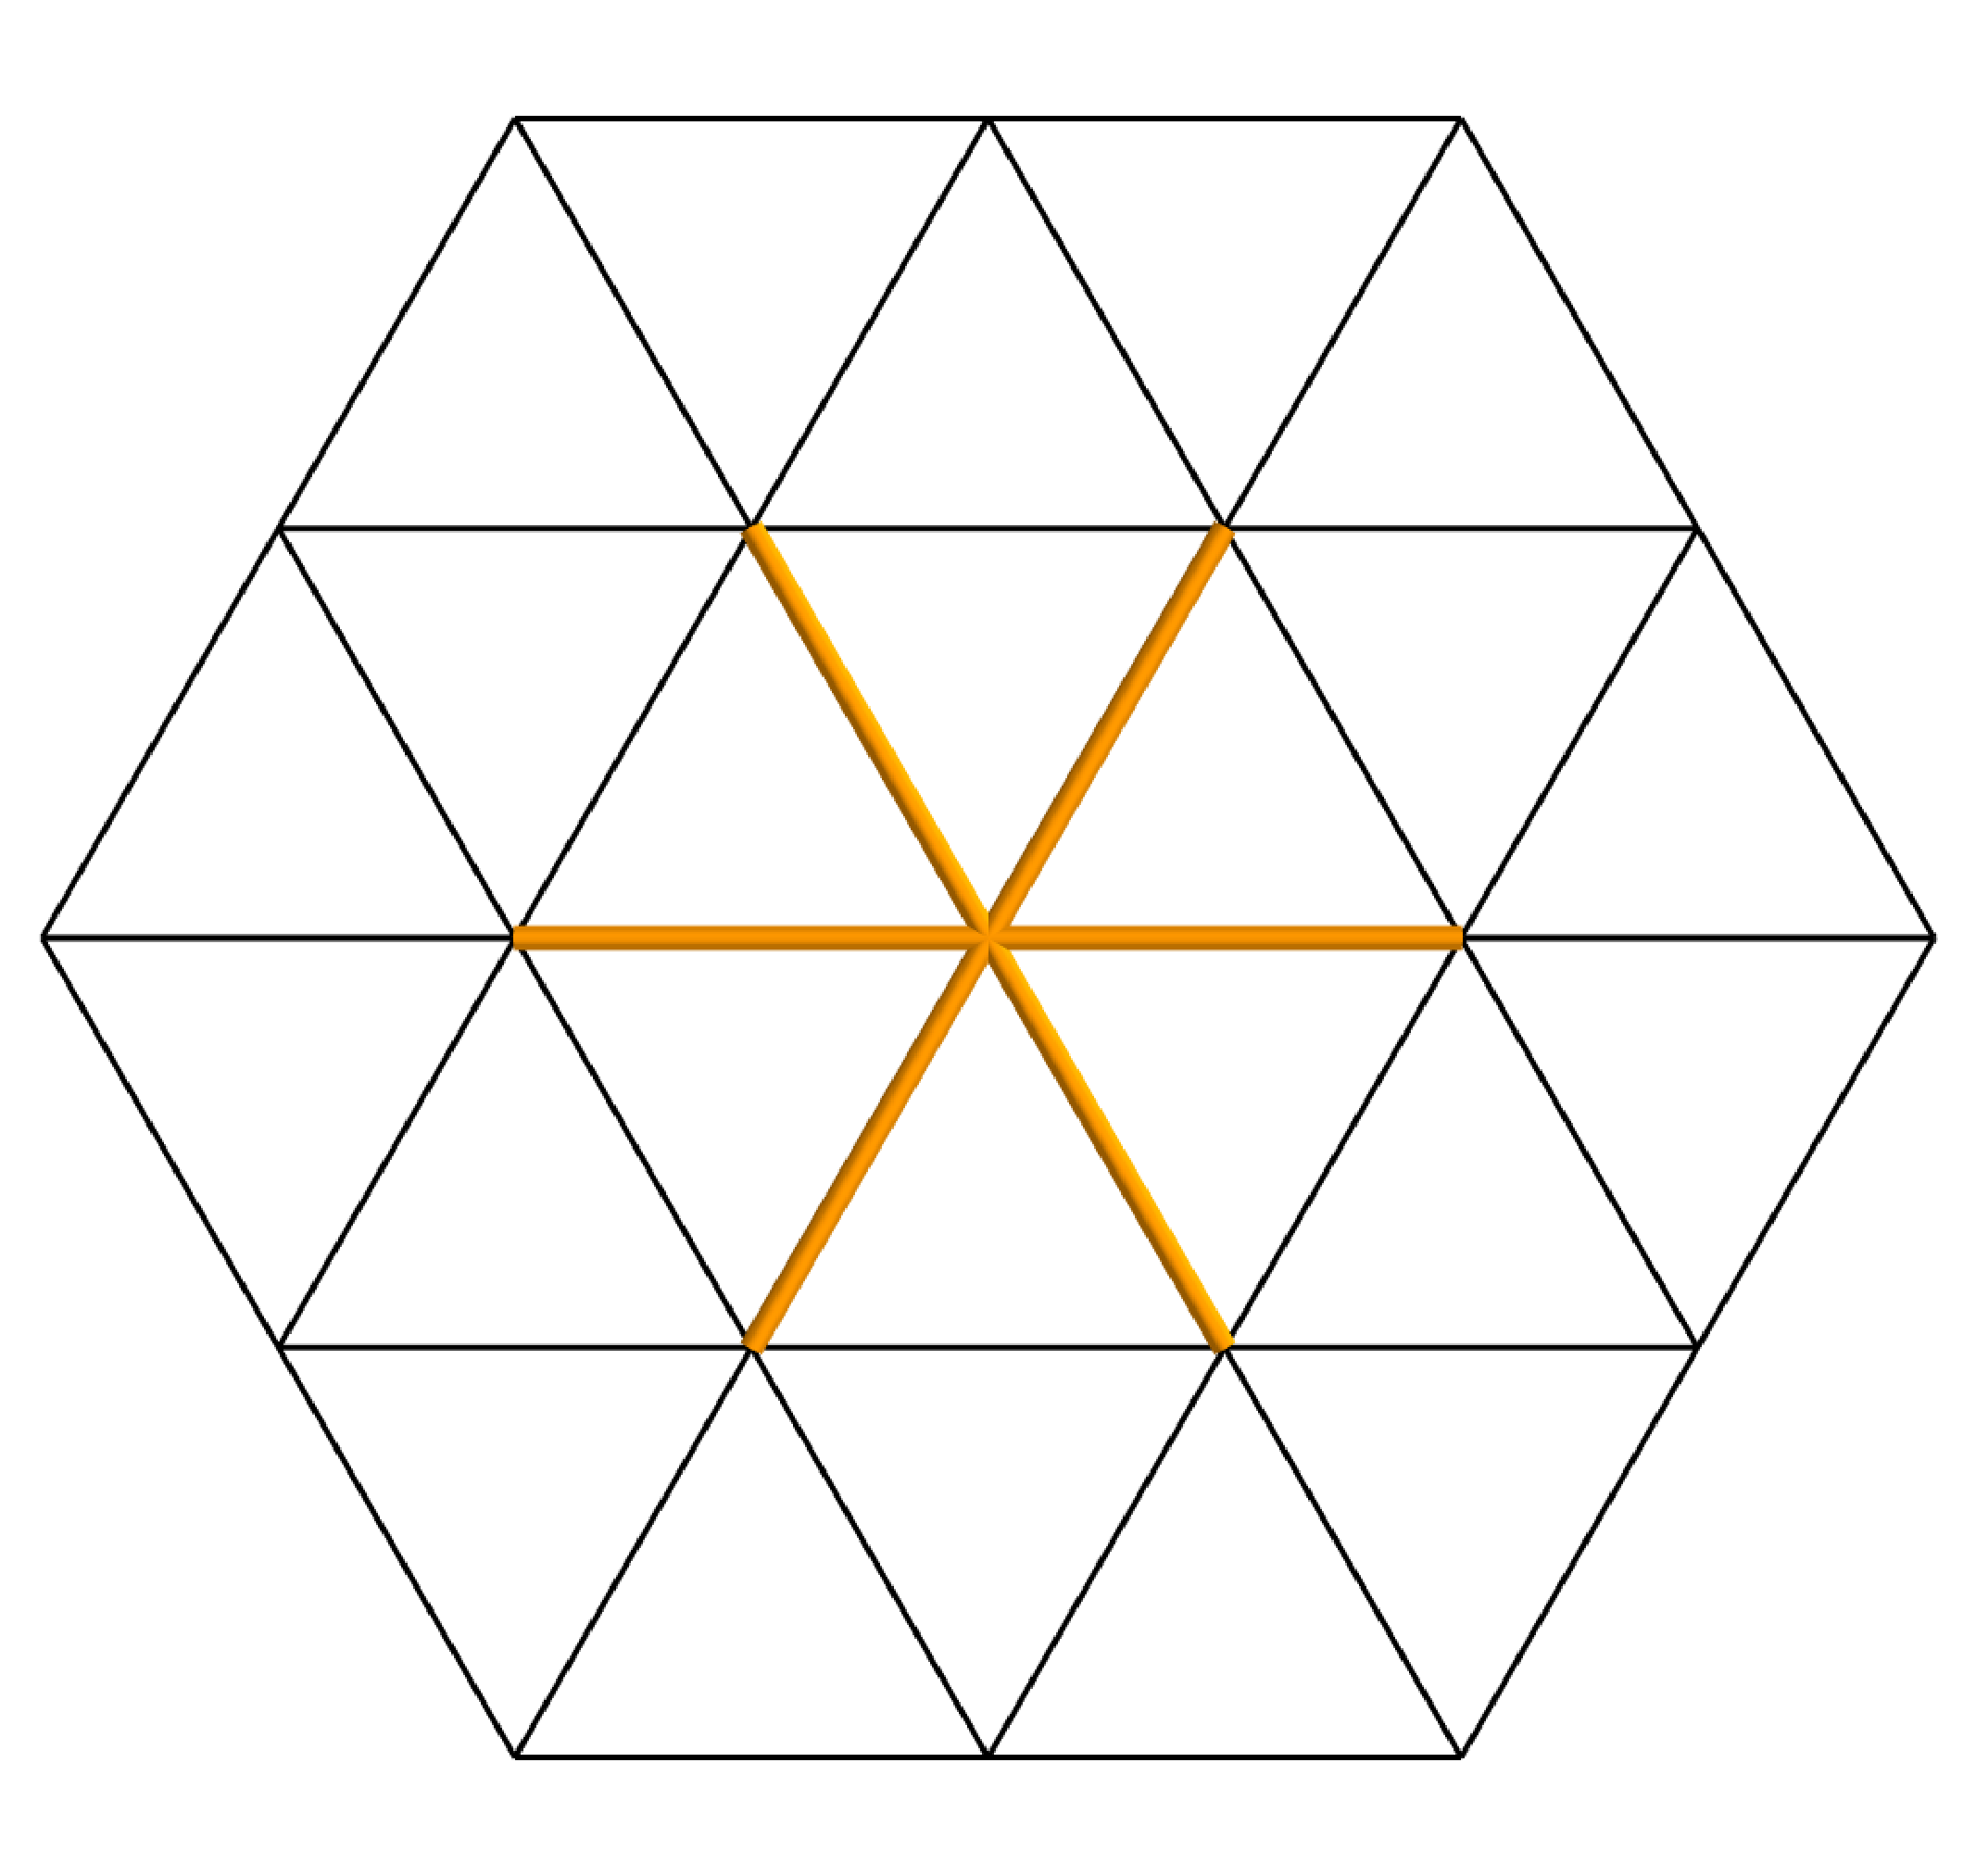
\includegraphics[width=0.25\textwidth]{images/stencils/0_form_deriv_stencil.pdf}};

\node (B2) at (\xB, \yTwo)
    {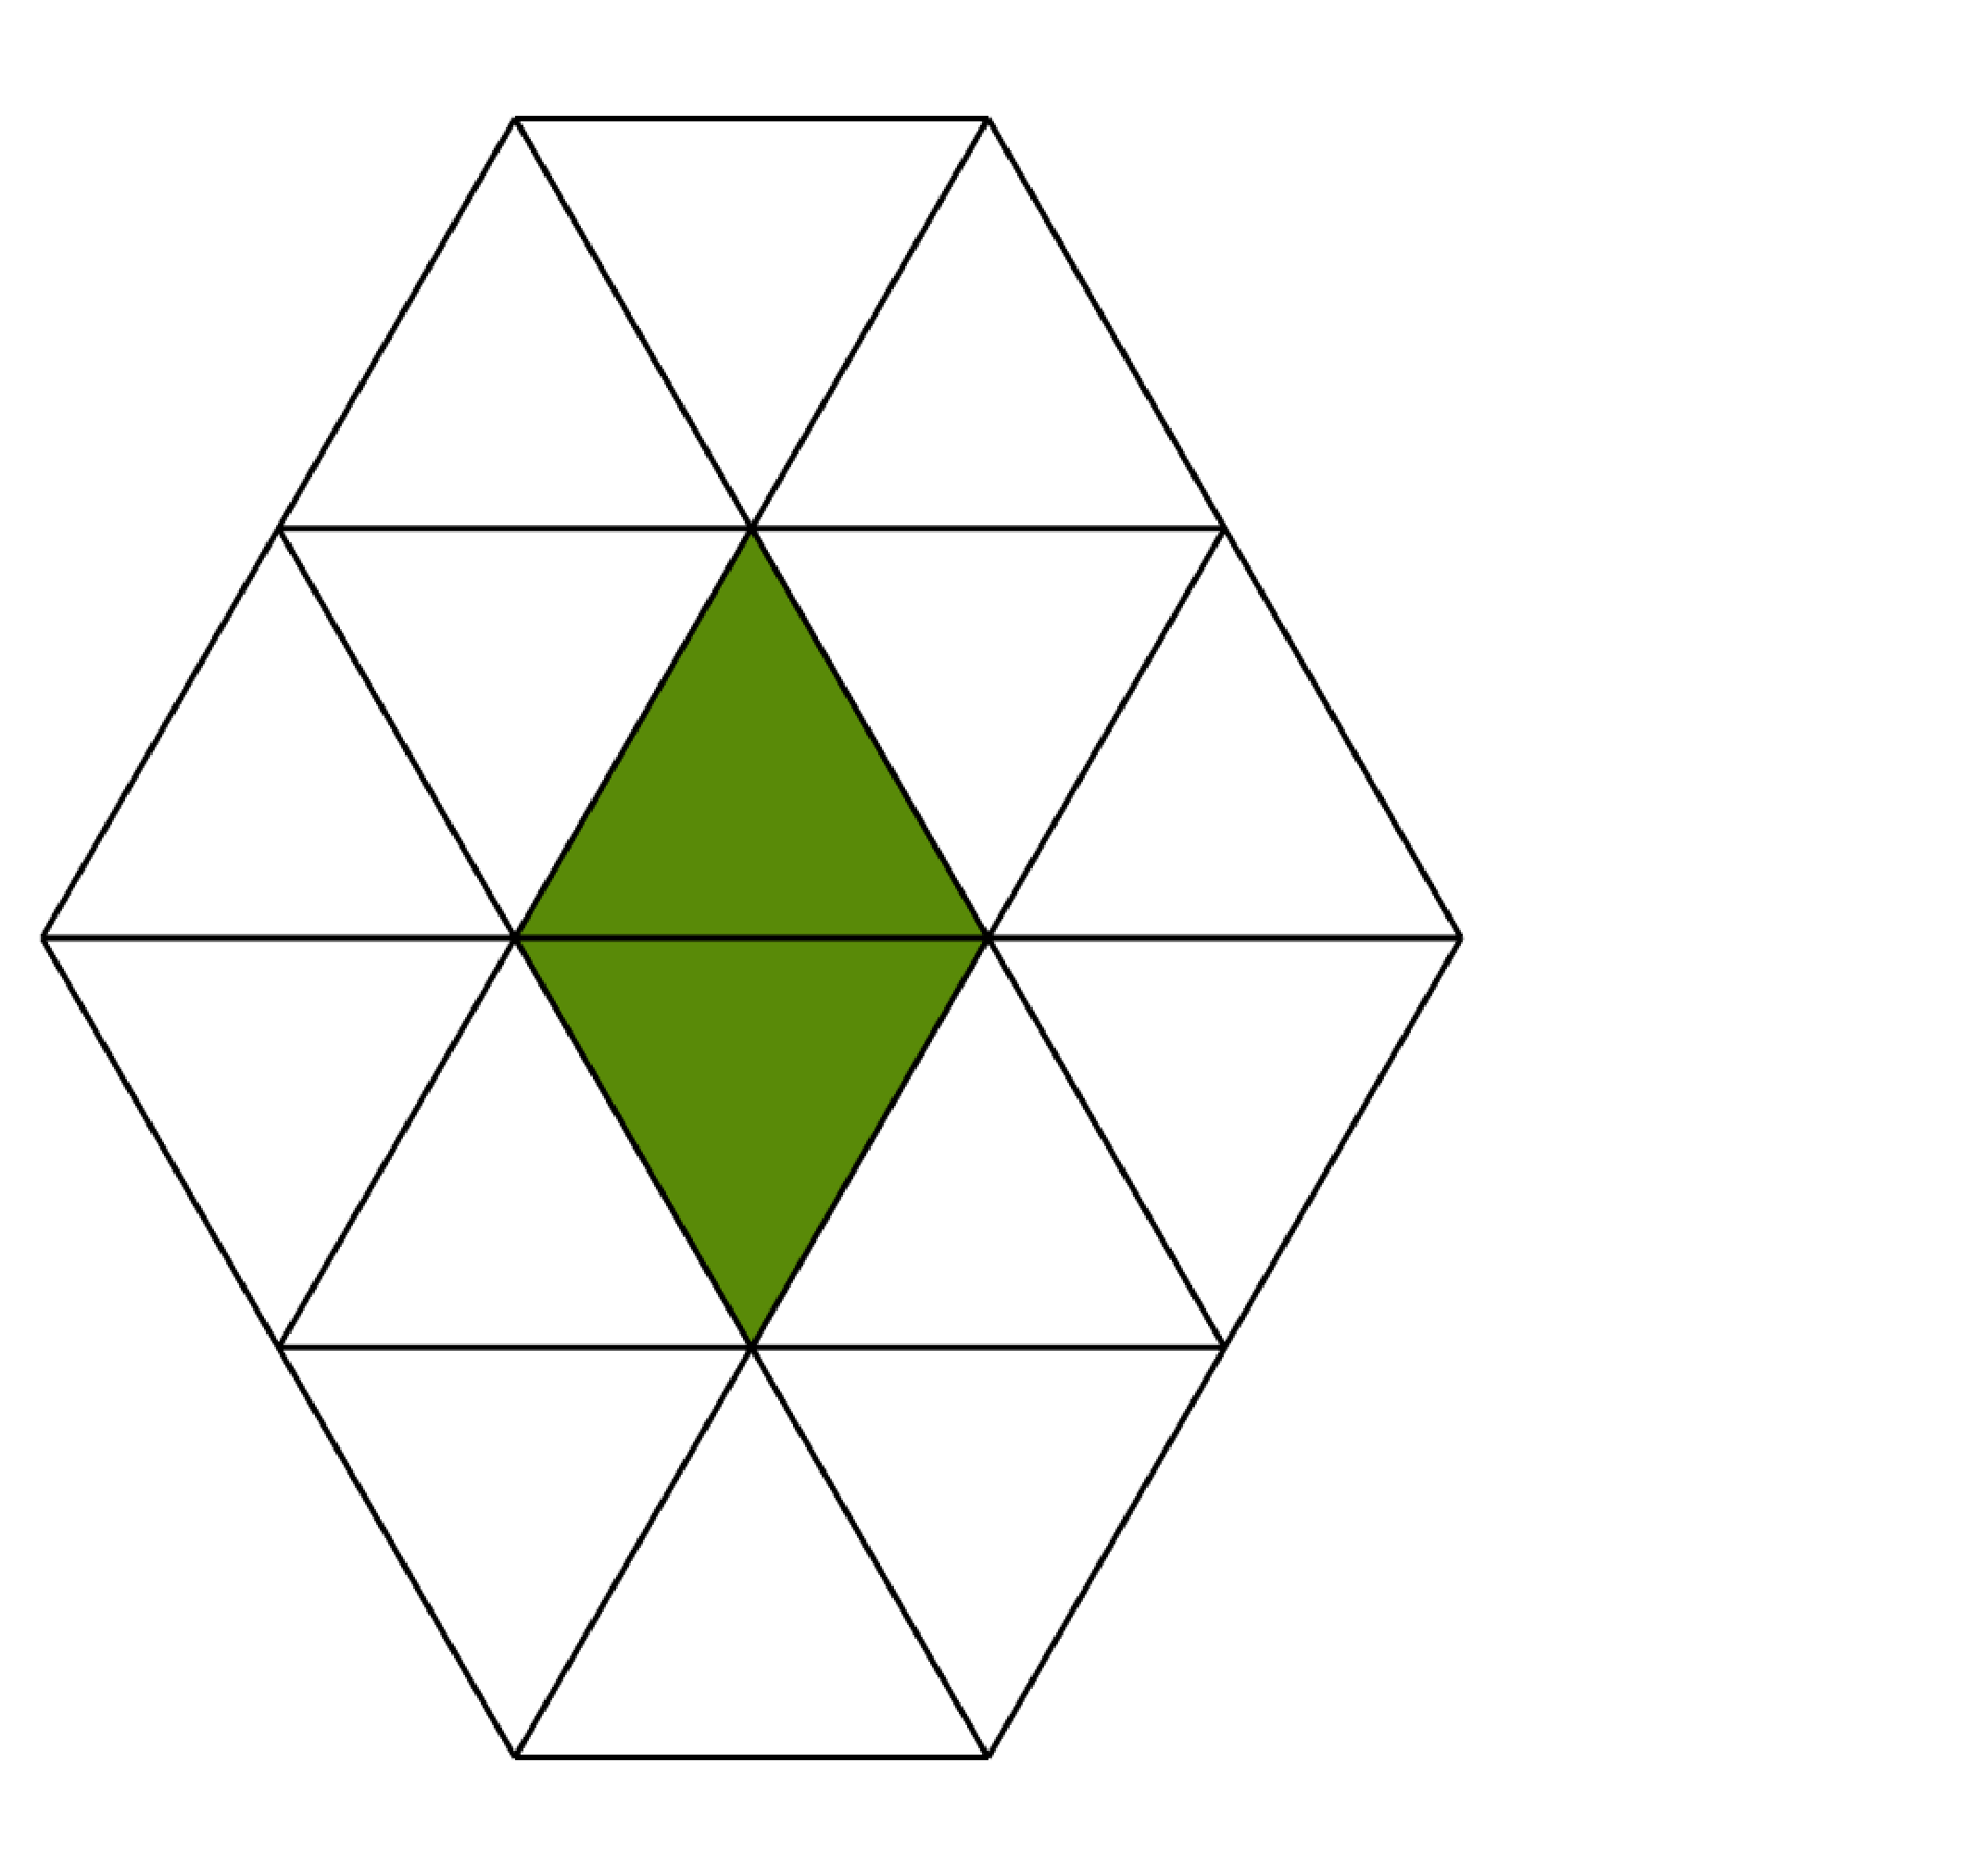
\includegraphics[width=0.25\textwidth, trim=10pt 0pt 10pt 0pt, clip]{images/stencils/1_form_deriv_stencil.pdf}};

\draw[arr] (A1.south) -- (A2.north) node[midway, right, font=\small] {$\;\;\DSt\big( \simplex{0}{\l}{\coarseIdxone} \big)$};
\draw[arr] ([xshift=-14pt]B1.south) -- ([xshift=-14pt]B2.north) node[midway, right, font=\small] {$\;\;\DSt\big( \simplex{1}{\l}{\coarseIdxone} \big)$};

\end{tikzpicture}
\end{center}
\vspace{-5mm}
\caption{Derivative stencils of $0$- and $1$-form basis functions.}
\end{figure}

\FloatBarrier

\subsection{Selecting active DoFs}

Active DoFs are determined through a \emph{subdivision partition}, a decomposition of the domain into patches on different refinement levels. For every patch, we add its simplices to the active $k$-form DoFs. We also need to add extra layers of fine interface DoFs on the coarse side of a coarse-fine interface to maintain a differential complex (cf. derivative stencil). The following figure provides a toy example to illustrate the resulting active DoFs.

\begin{figure}[H]
\begin{center}
\begin{tikzpicture}[
    every node/.style={inner sep=0pt, outer sep=0pt},
    arr/.style={->, >=Stealth, line width=1.5pt, shorten >=2pt, shorten <=2pt}
]

\def\xA{0cm}
\def\xB{3.9cm}
\def\xC{7.8cm}
\def\yOne{0cm}
\def\yTwo{-2.4cm}
\def\yThree{-4.8cm}

\node (A1) at (\xA, \yOne)
    {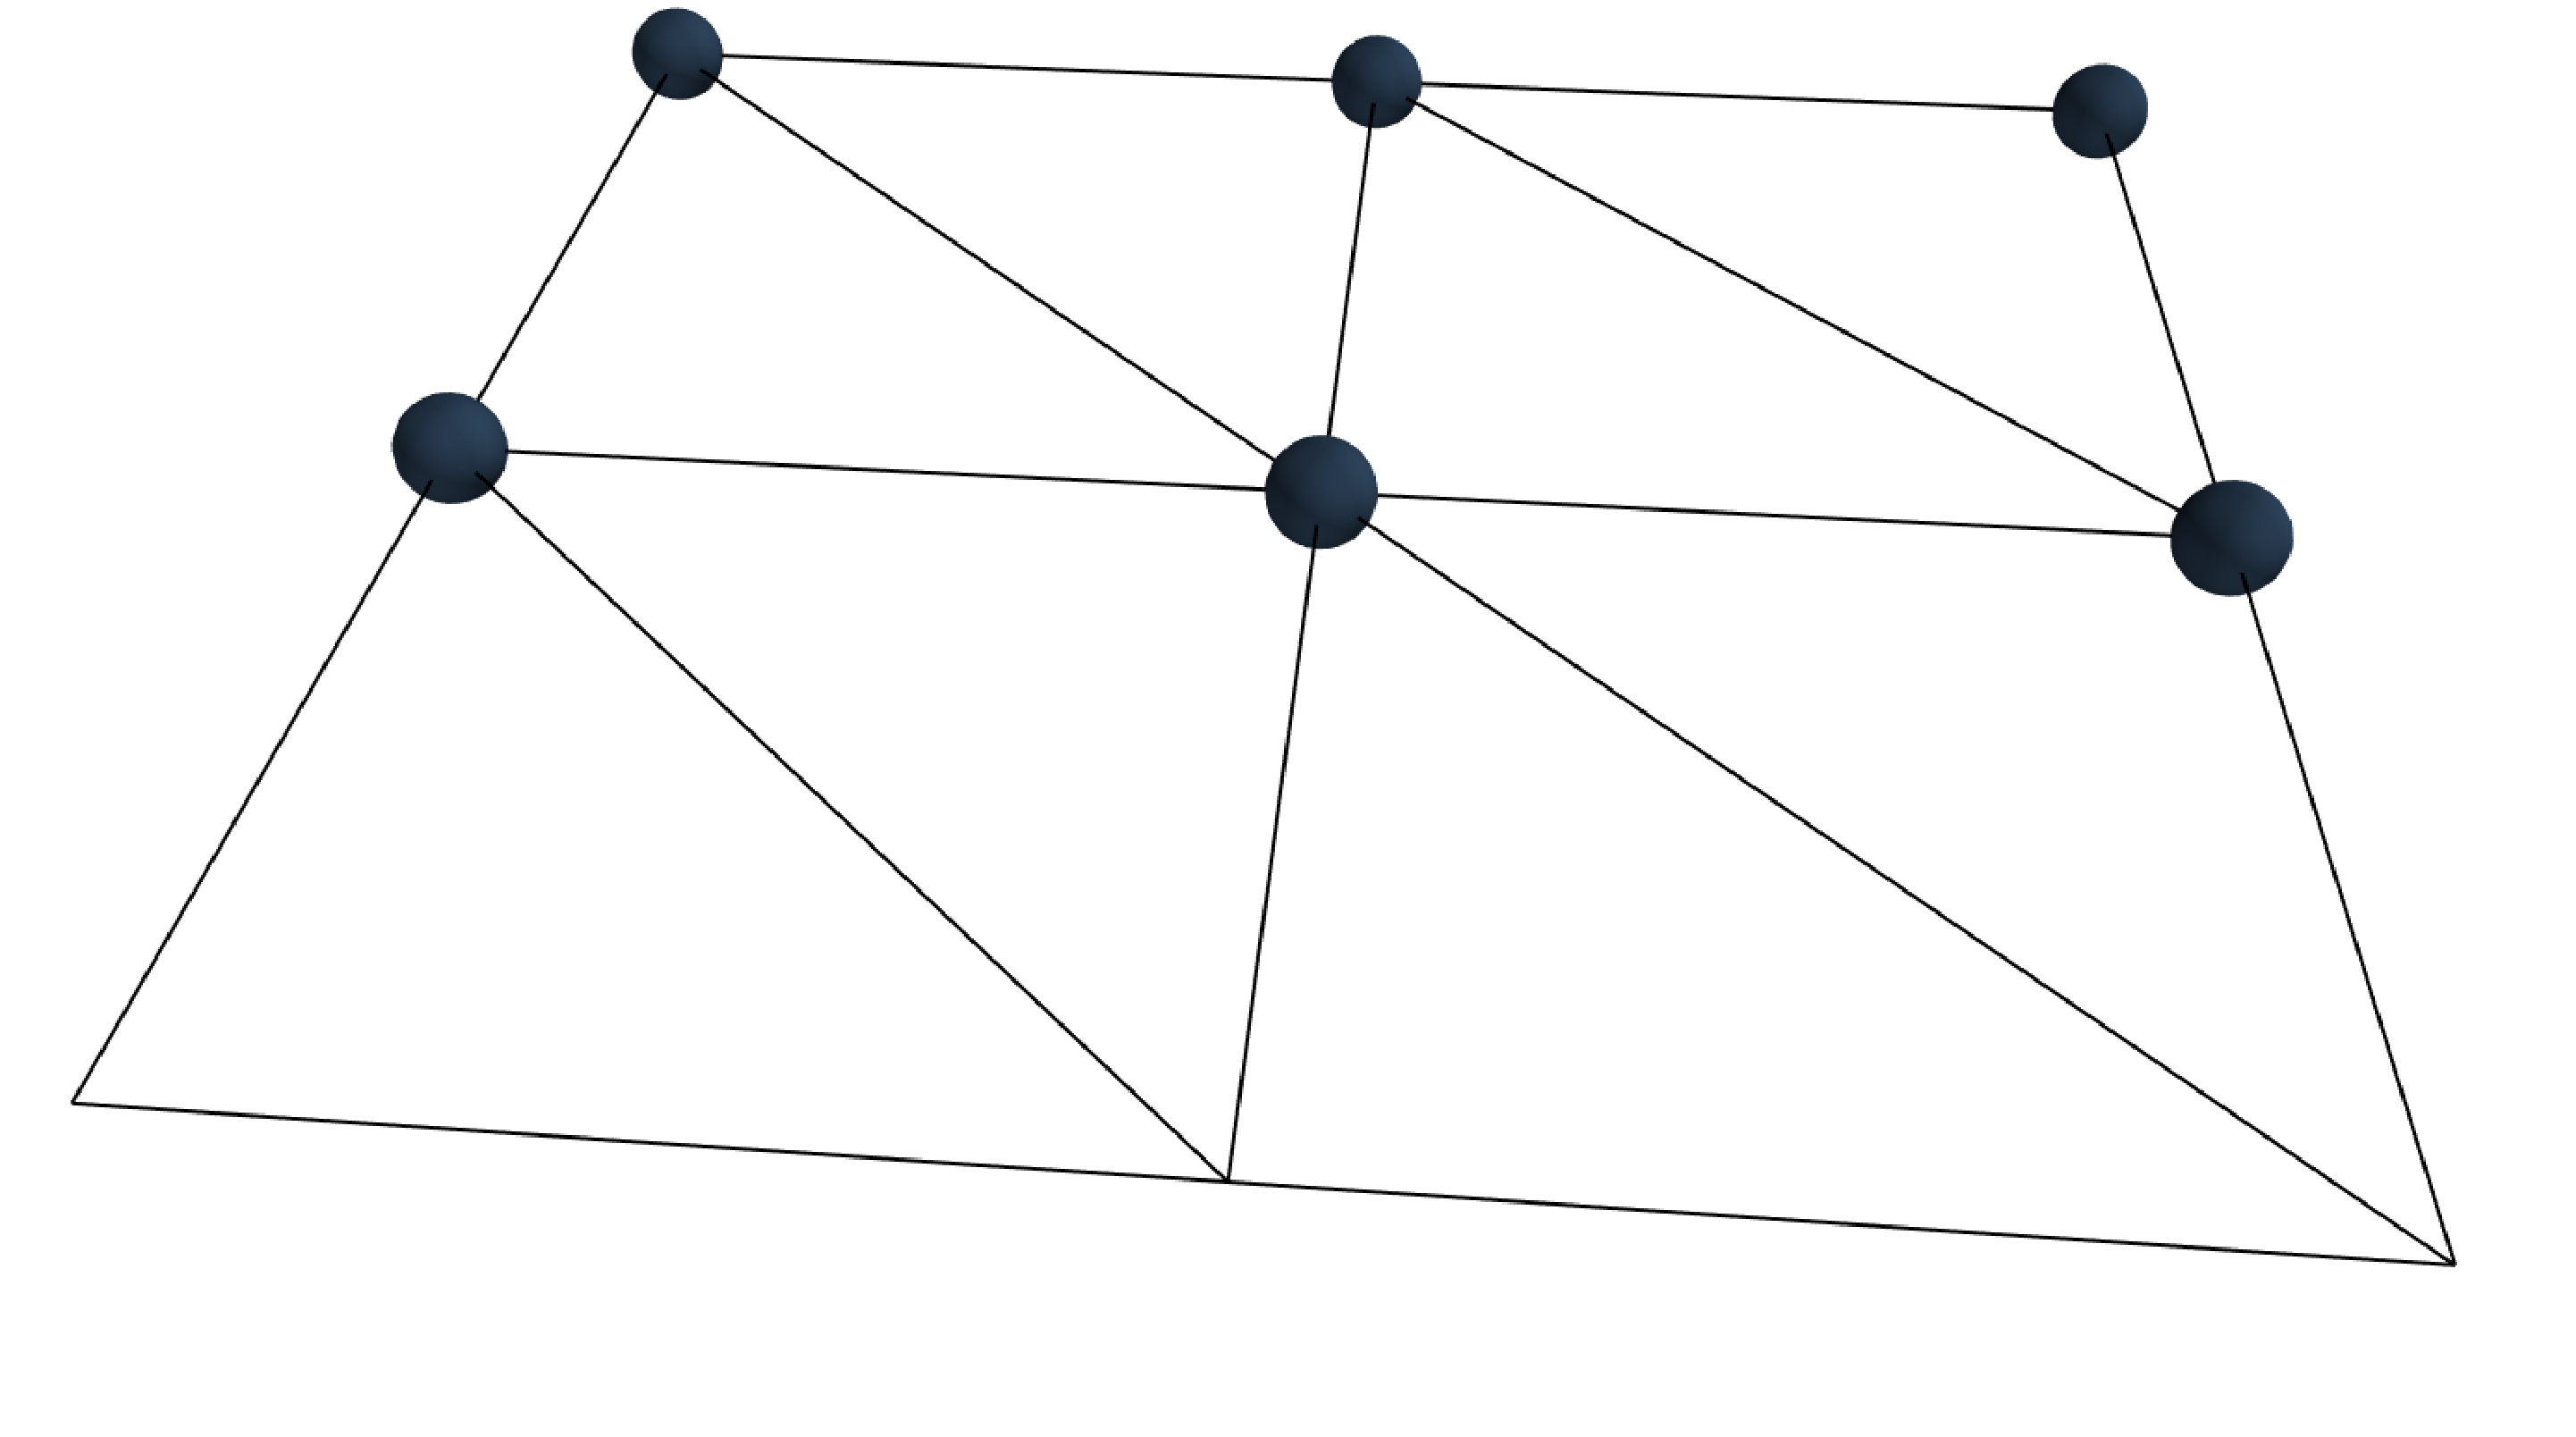
\includegraphics[width=0.22\textwidth]{images/dofmeshes/correct/dofs_k_0_lvl_l0.pdf}};

\node (B1) at (\xB, \yOne)
    {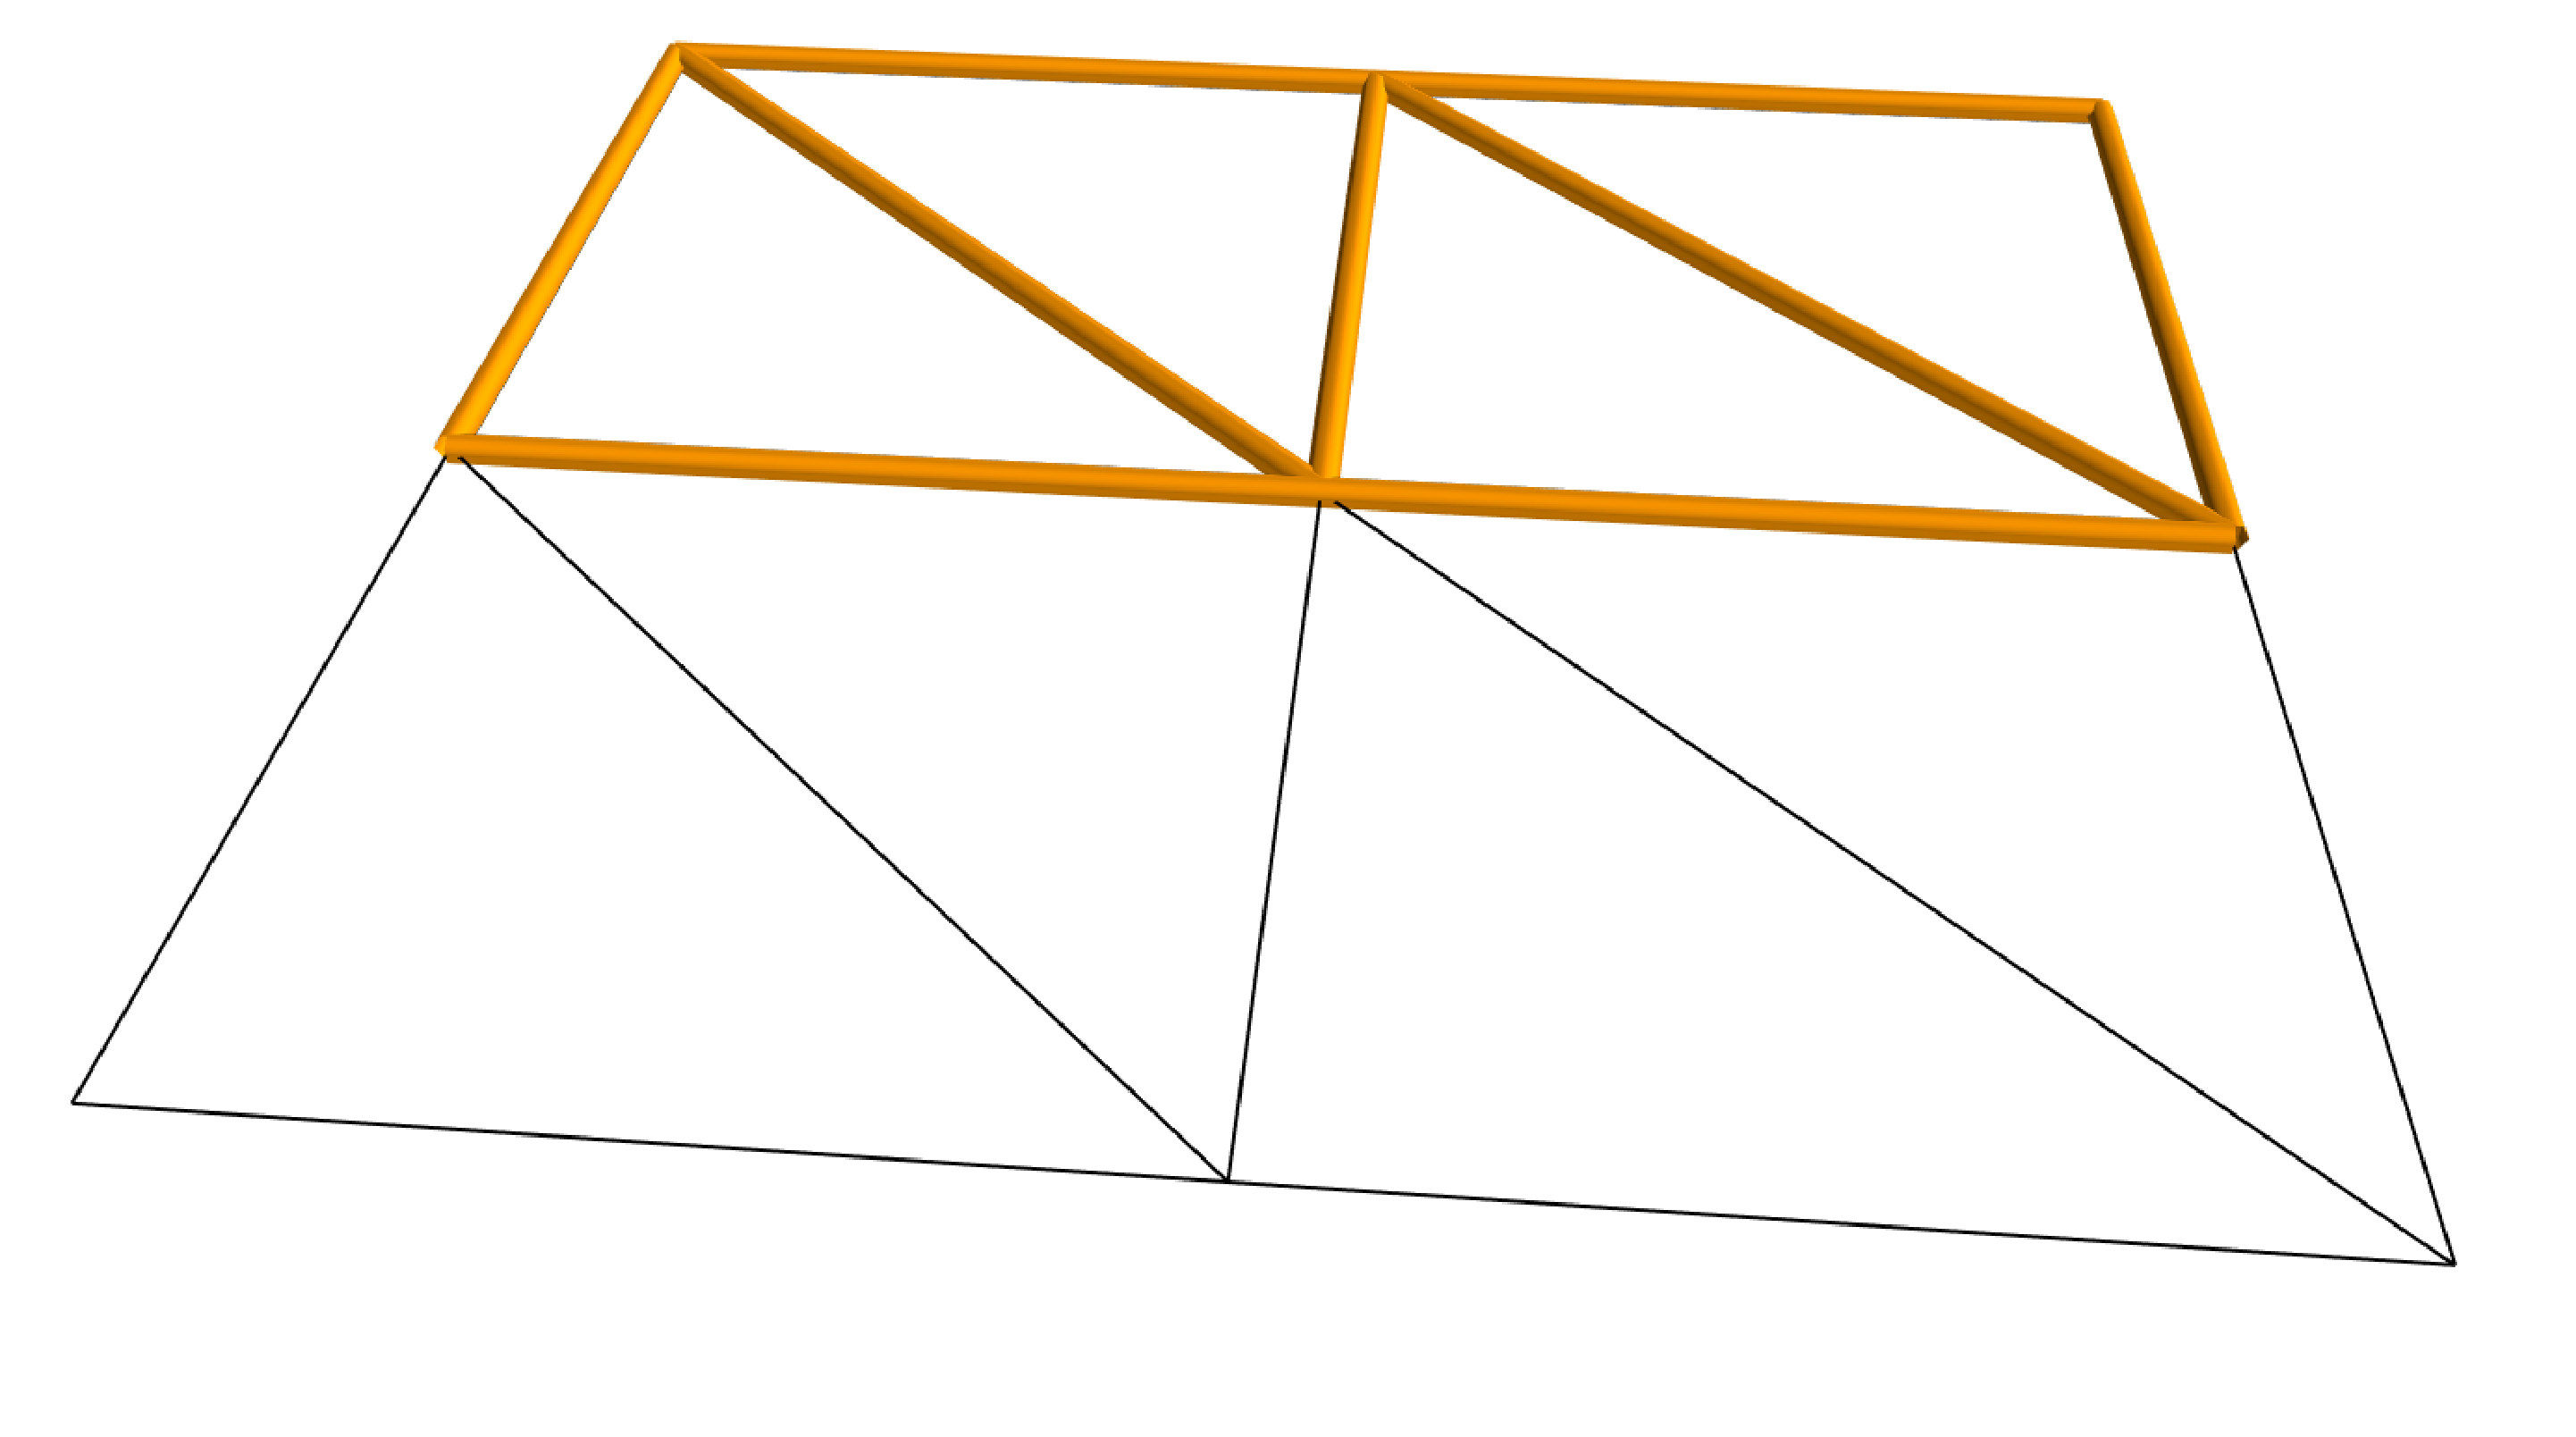
\includegraphics[width=0.22\textwidth, trim=10pt 0pt 10pt 0pt, clip]{images/dofmeshes/correct/dofs_k_1_lvl_l0.pdf}};

\node (C1) at (\xC, \yOne)
    {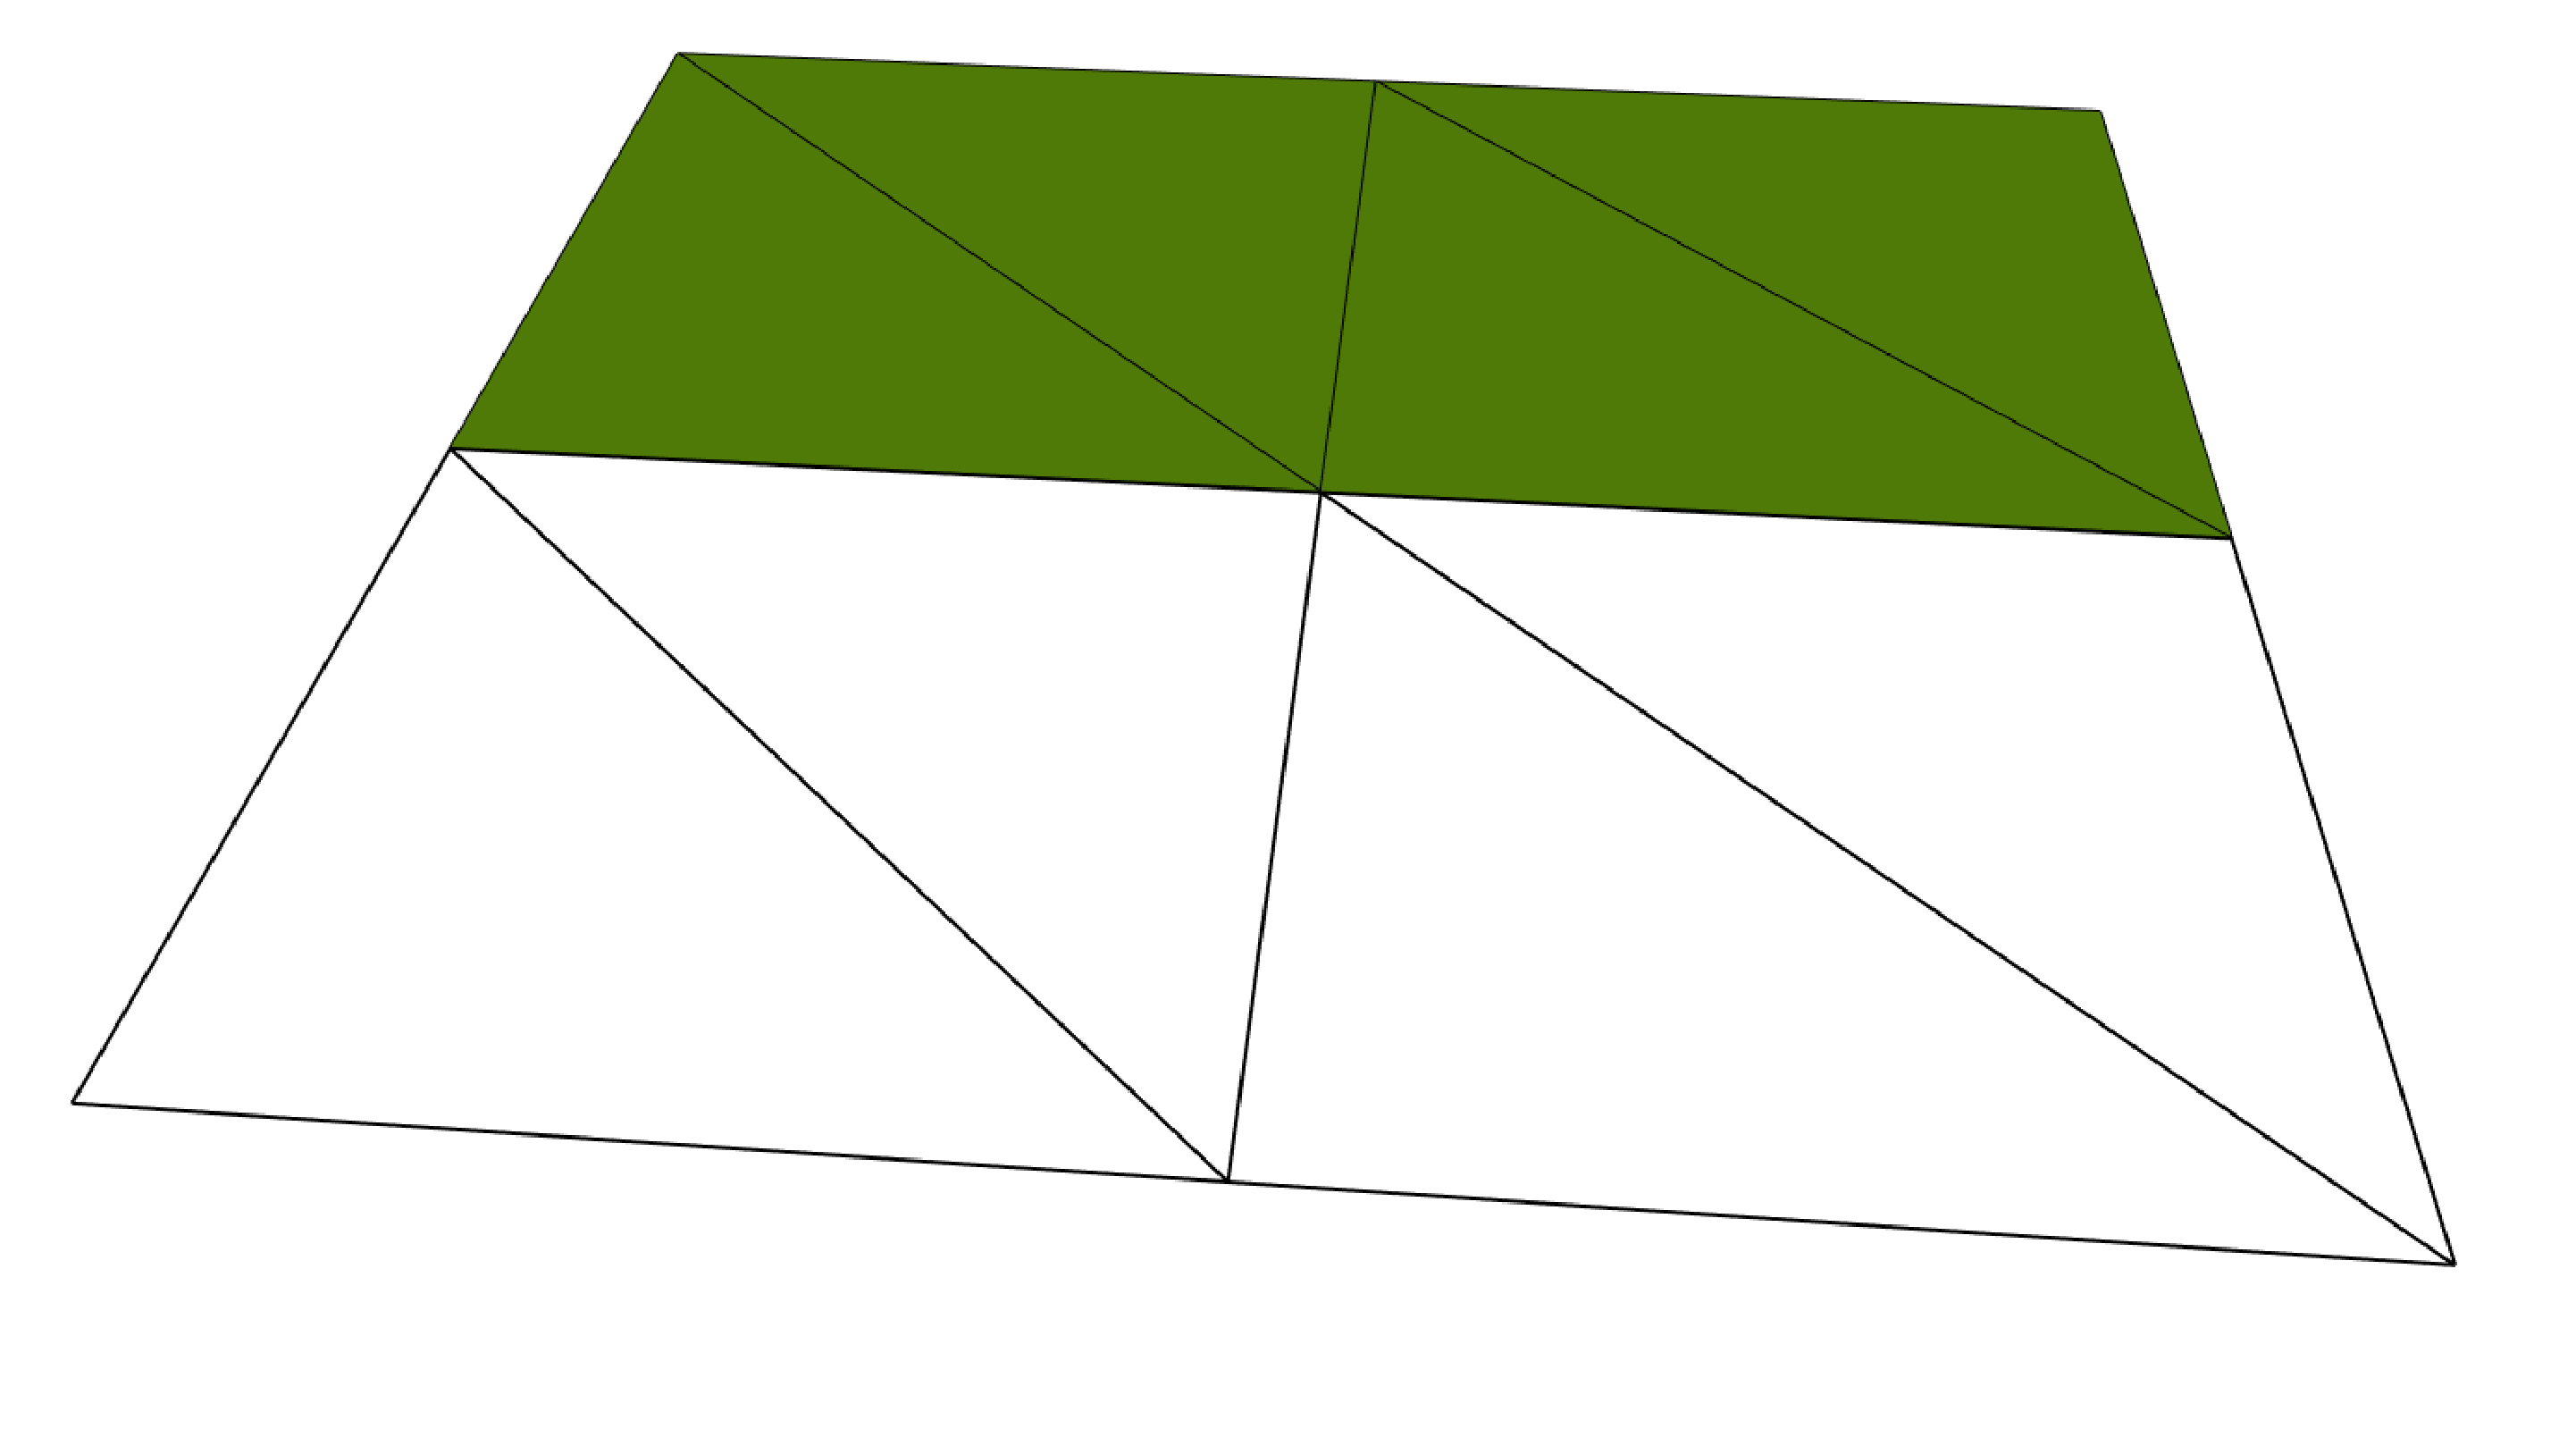
\includegraphics[width=0.22\textwidth]{images/dofmeshes/correct/dofs_k_2_lvl_l0.pdf}};

\node (A2) at (\xA, \yTwo)
    {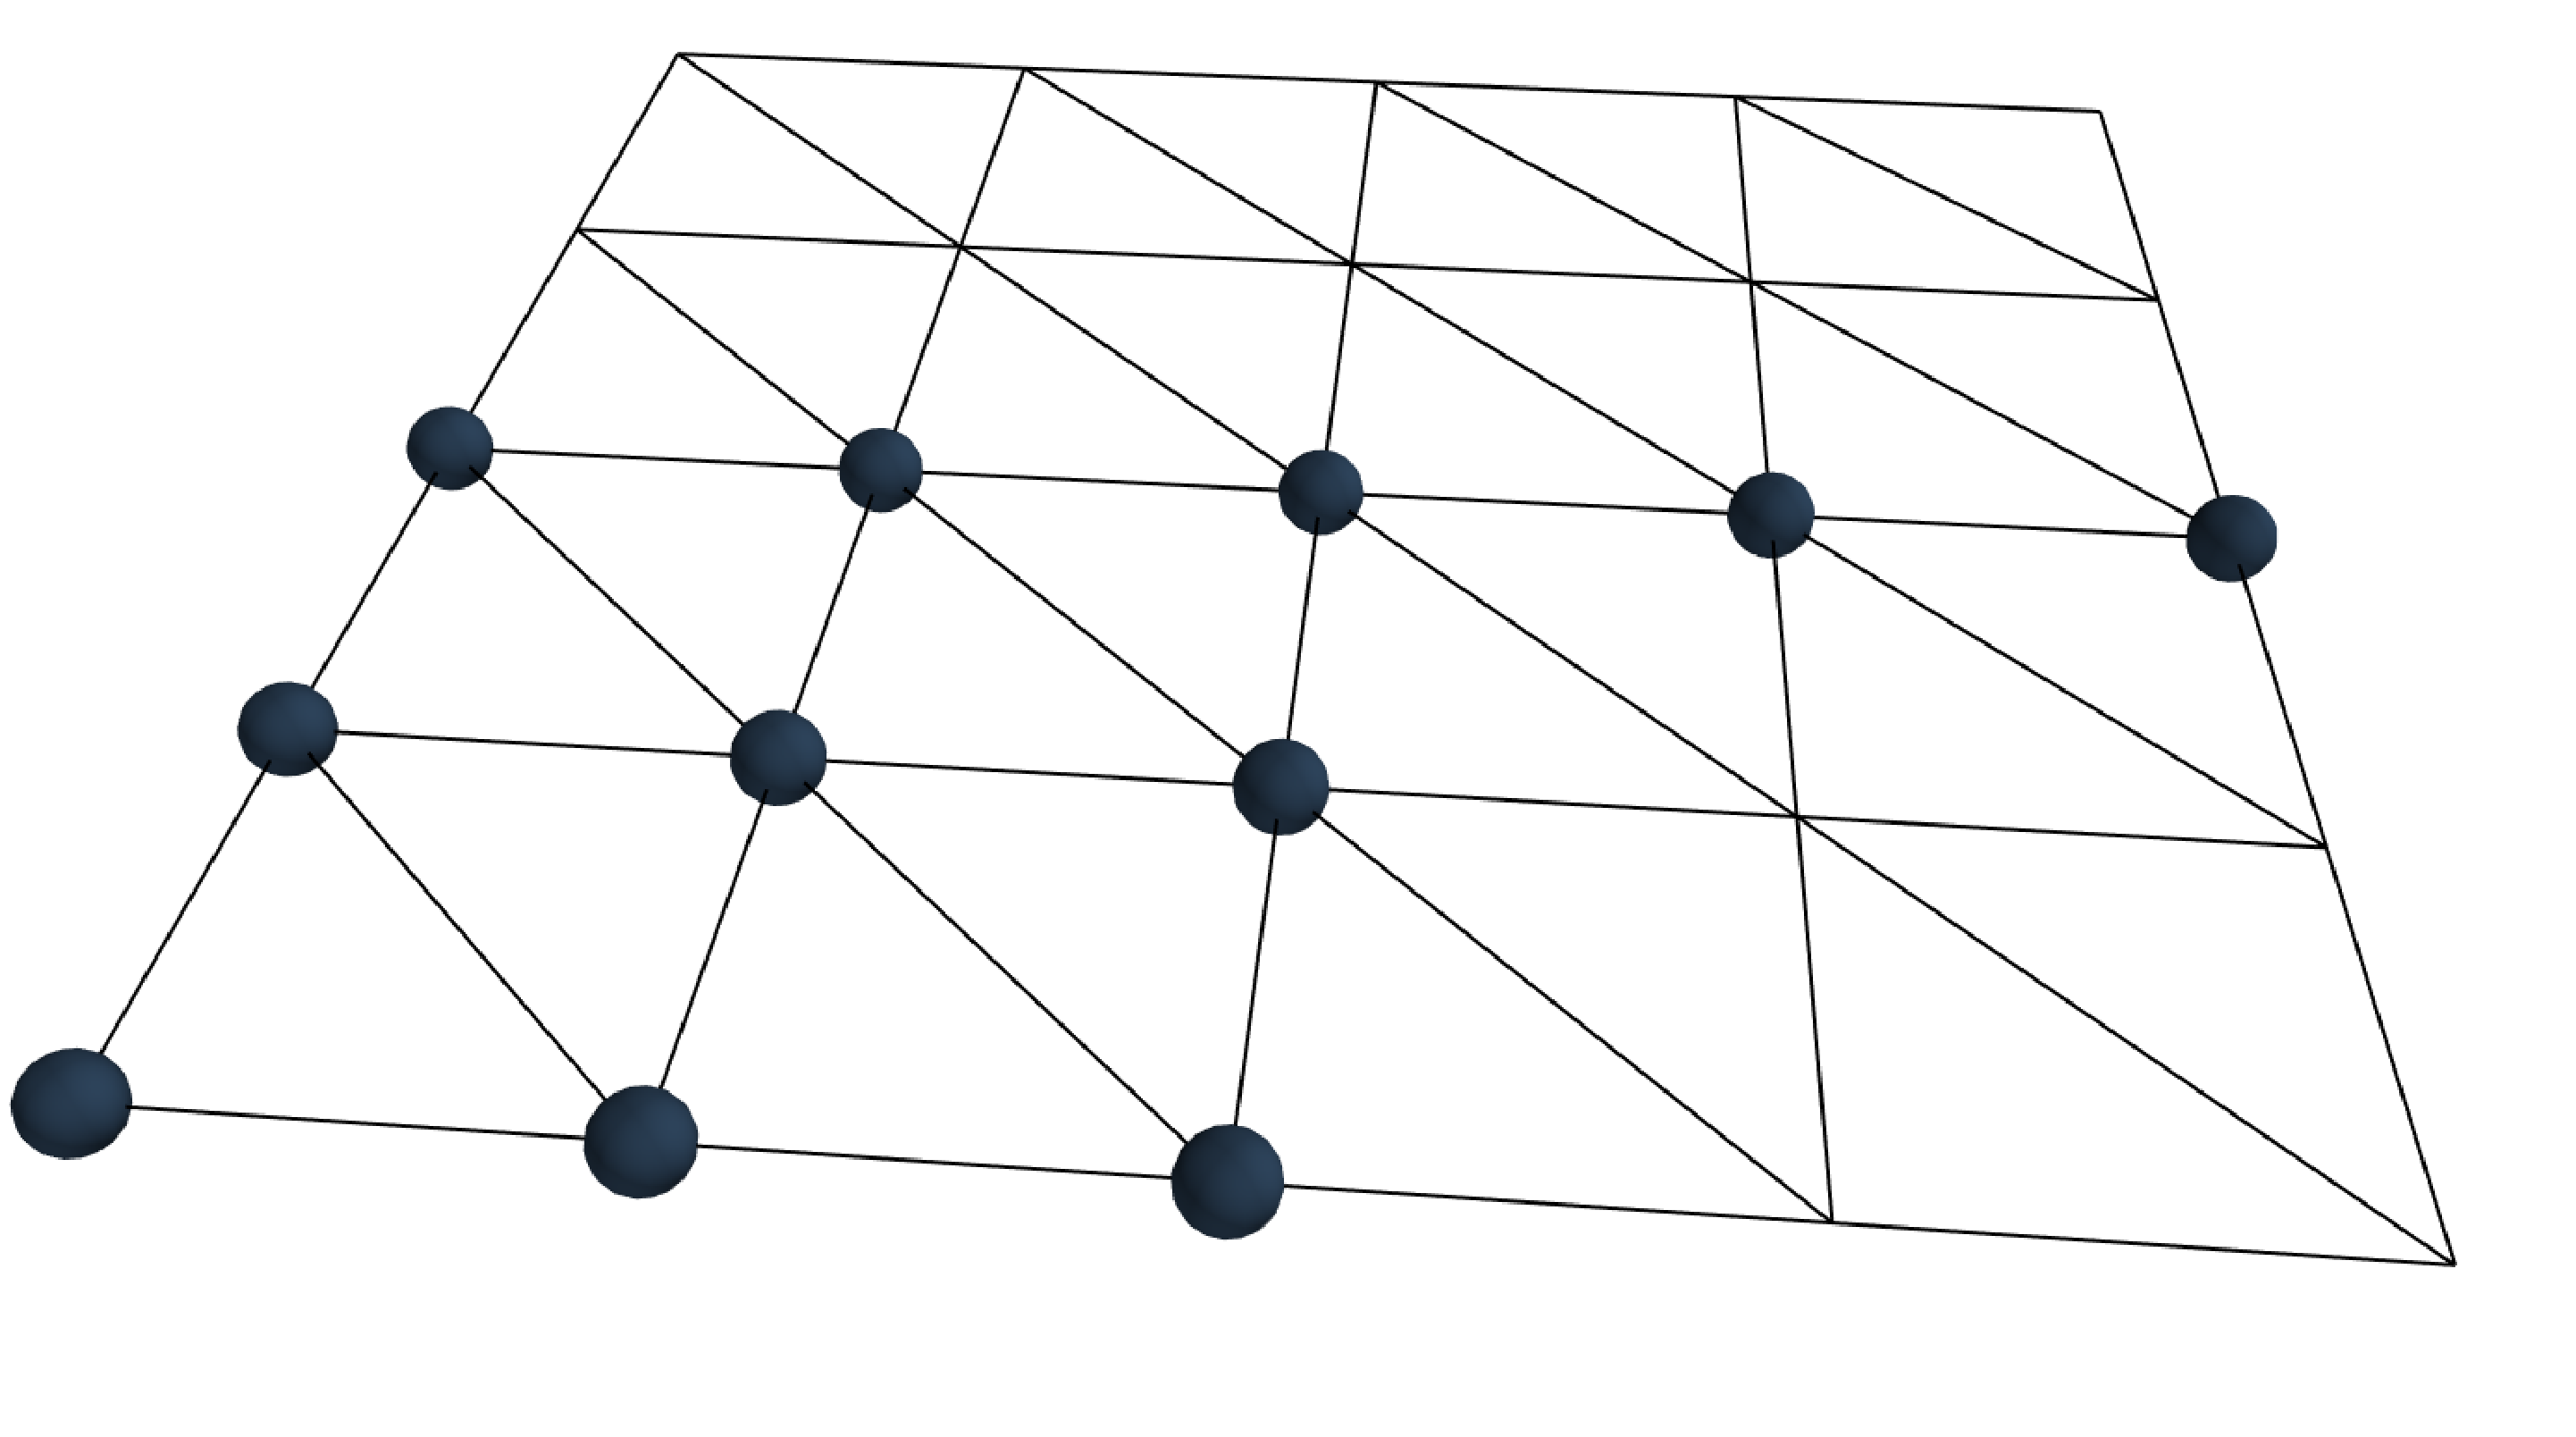
\includegraphics[width=0.22\textwidth]{images/dofmeshes/correct/dofs_k_0_lvl_l1.pdf}};

\node (B2) at (\xB, \yTwo)
    {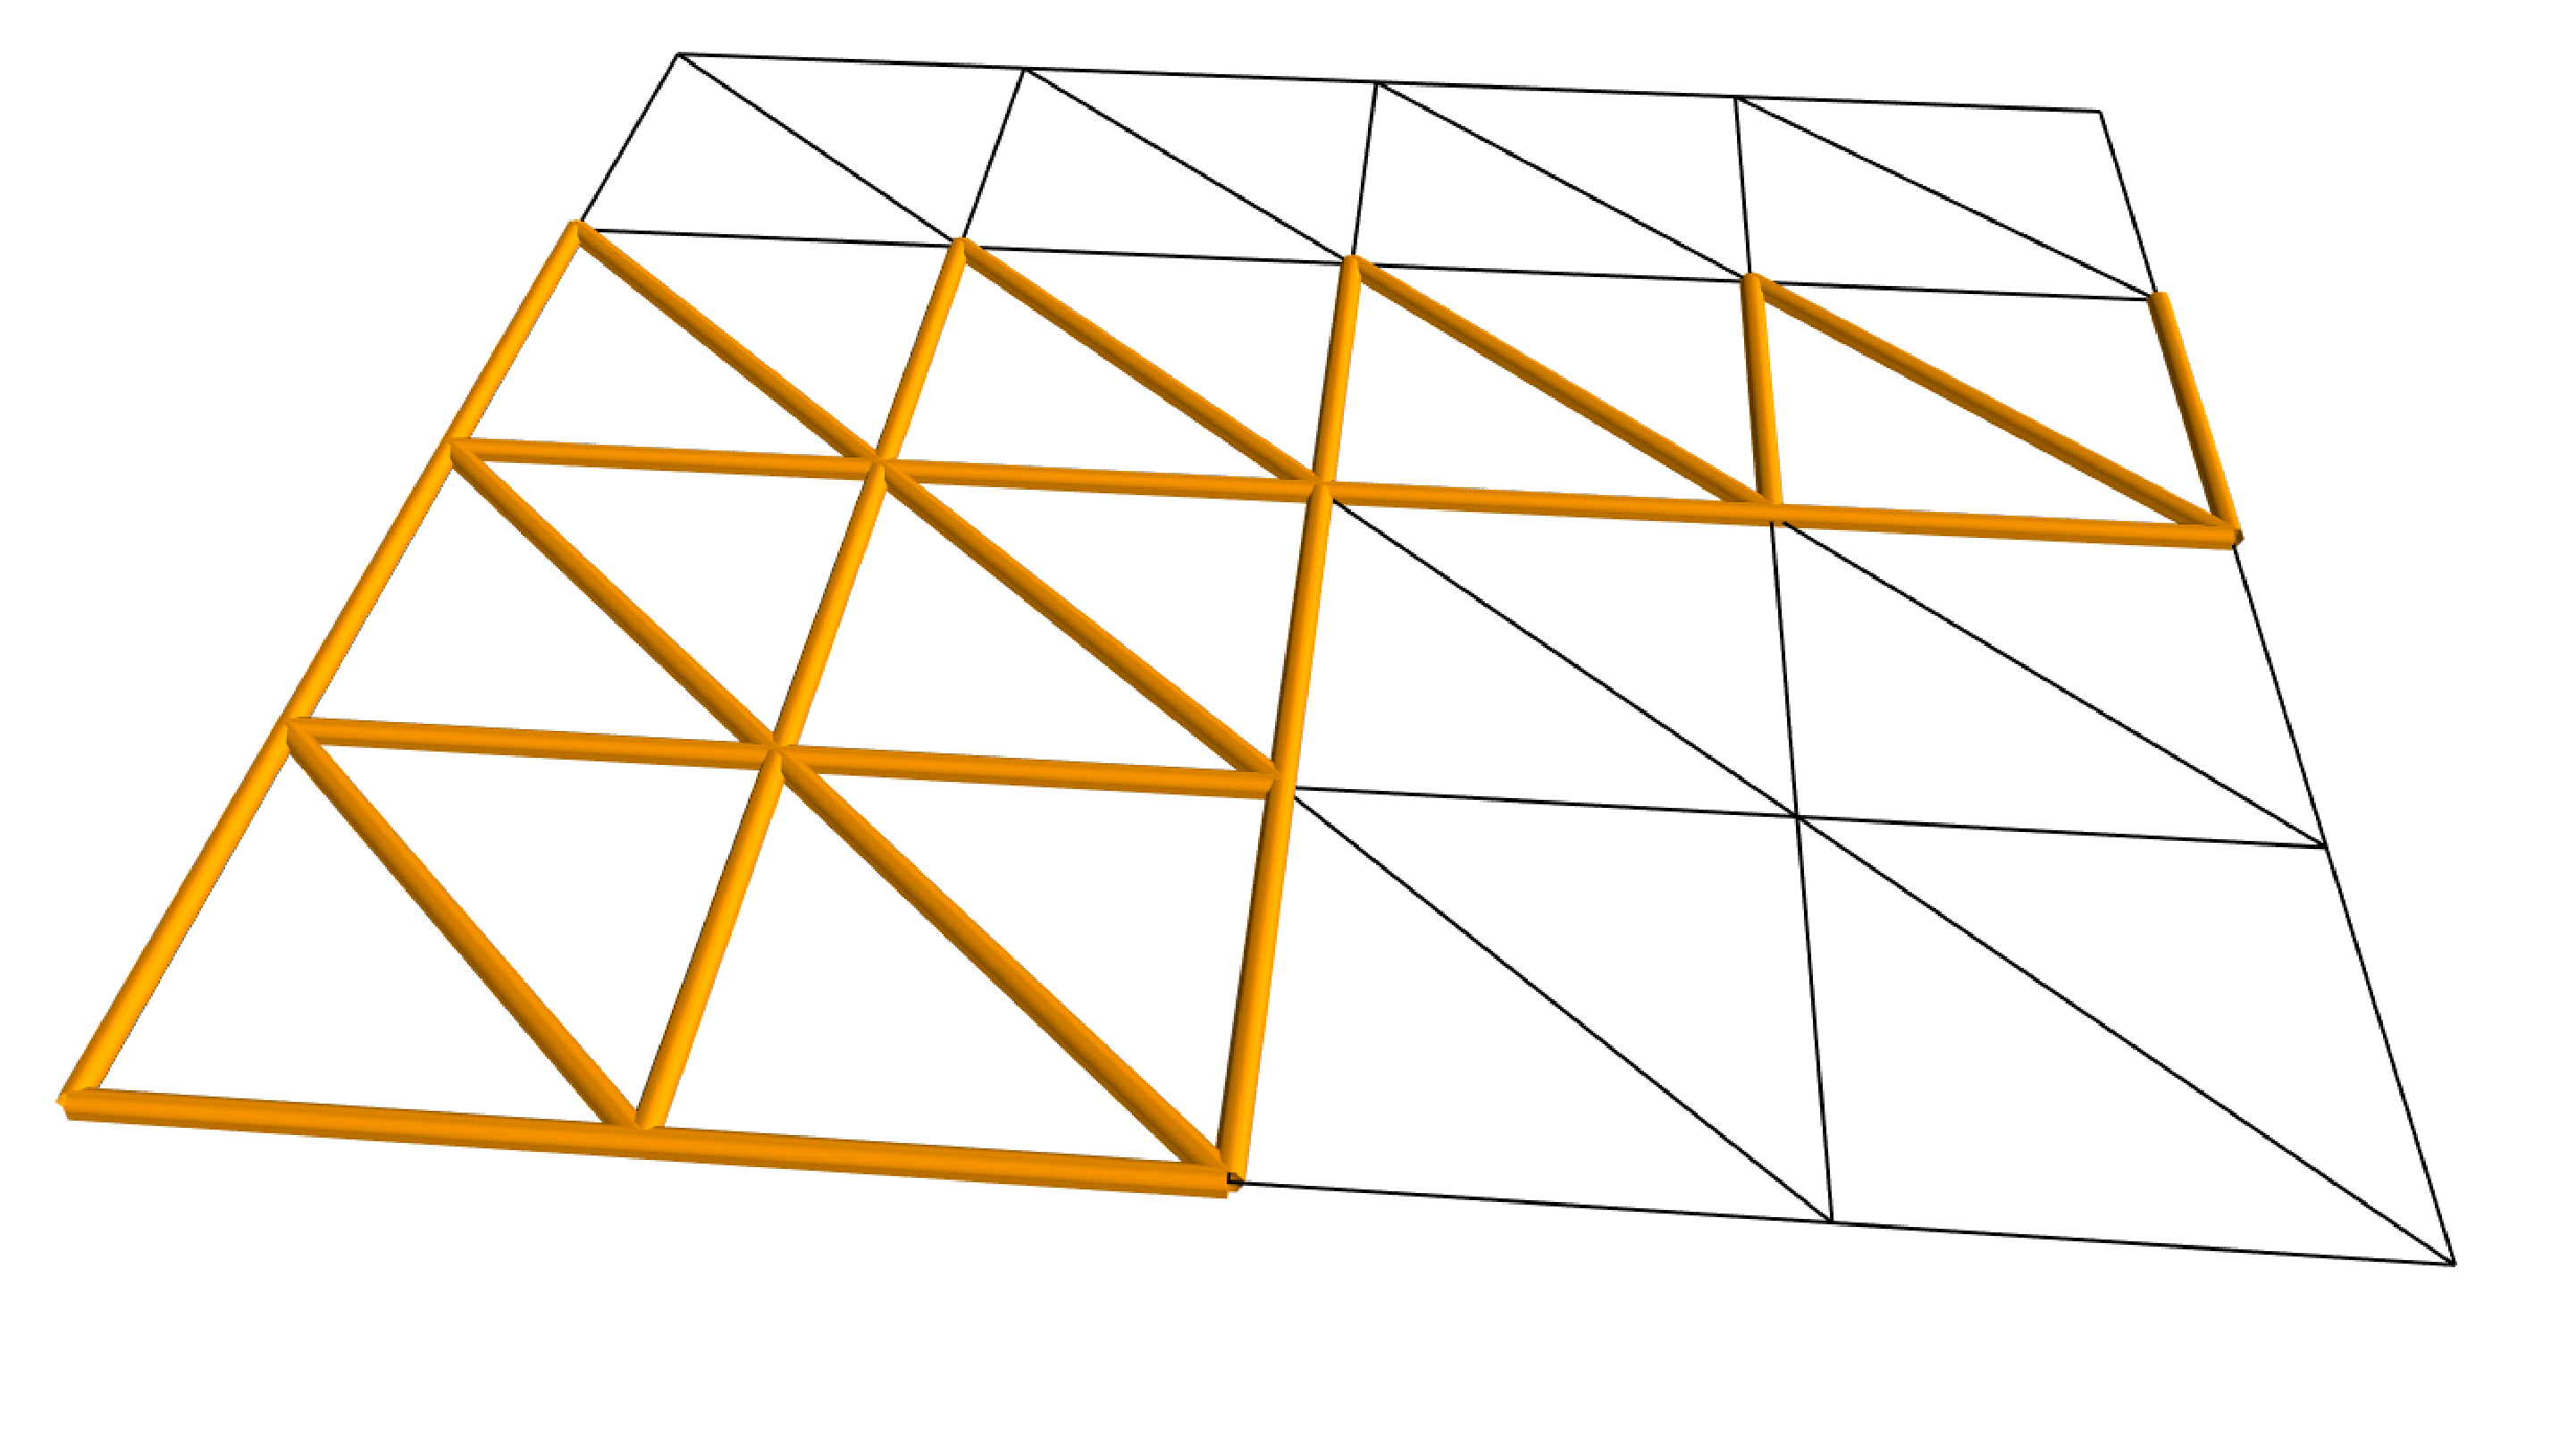
\includegraphics[width=0.22\textwidth, trim=10pt 0pt 10pt 0pt, clip]{images/dofmeshes/correct/dofs_k_1_lvl_l1.pdf}};

\node (C2) at (\xC, \yTwo)
    {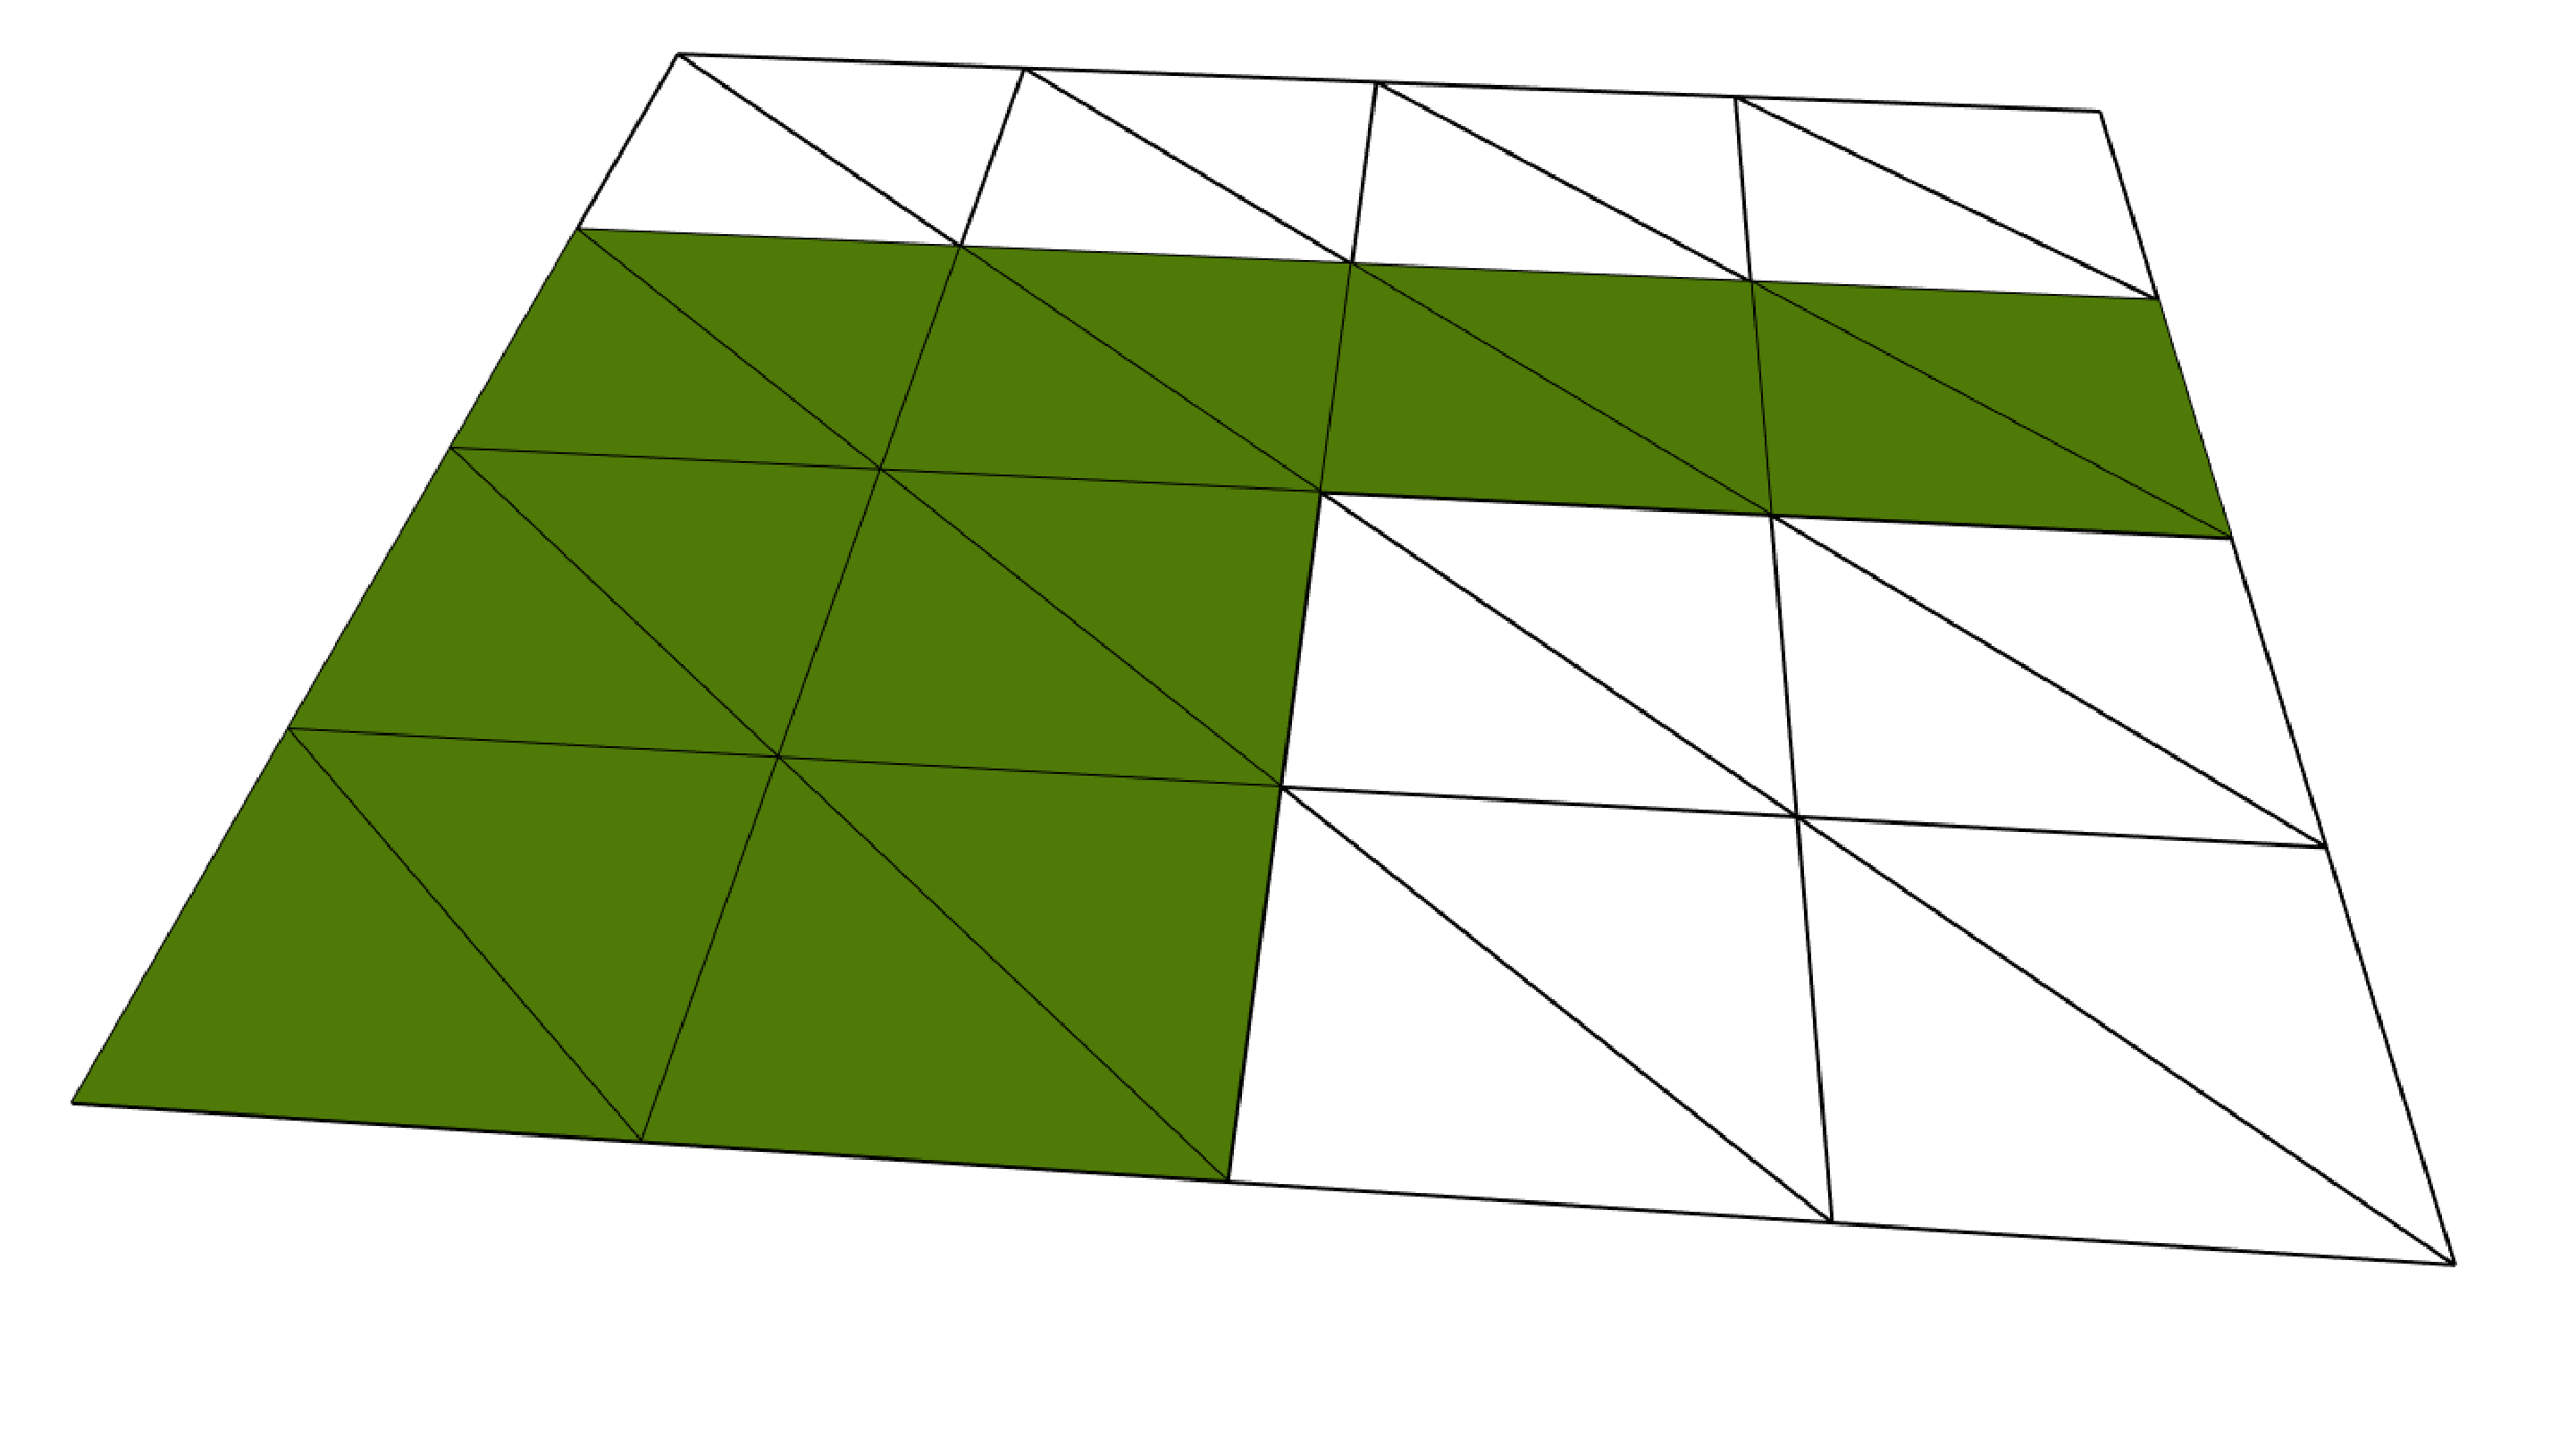
\includegraphics[width=0.22\textwidth]{images/dofmeshes/correct/dofs_k_2_lvl_l1.pdf}};

\node (A3) at (\xA, \yThree)
    {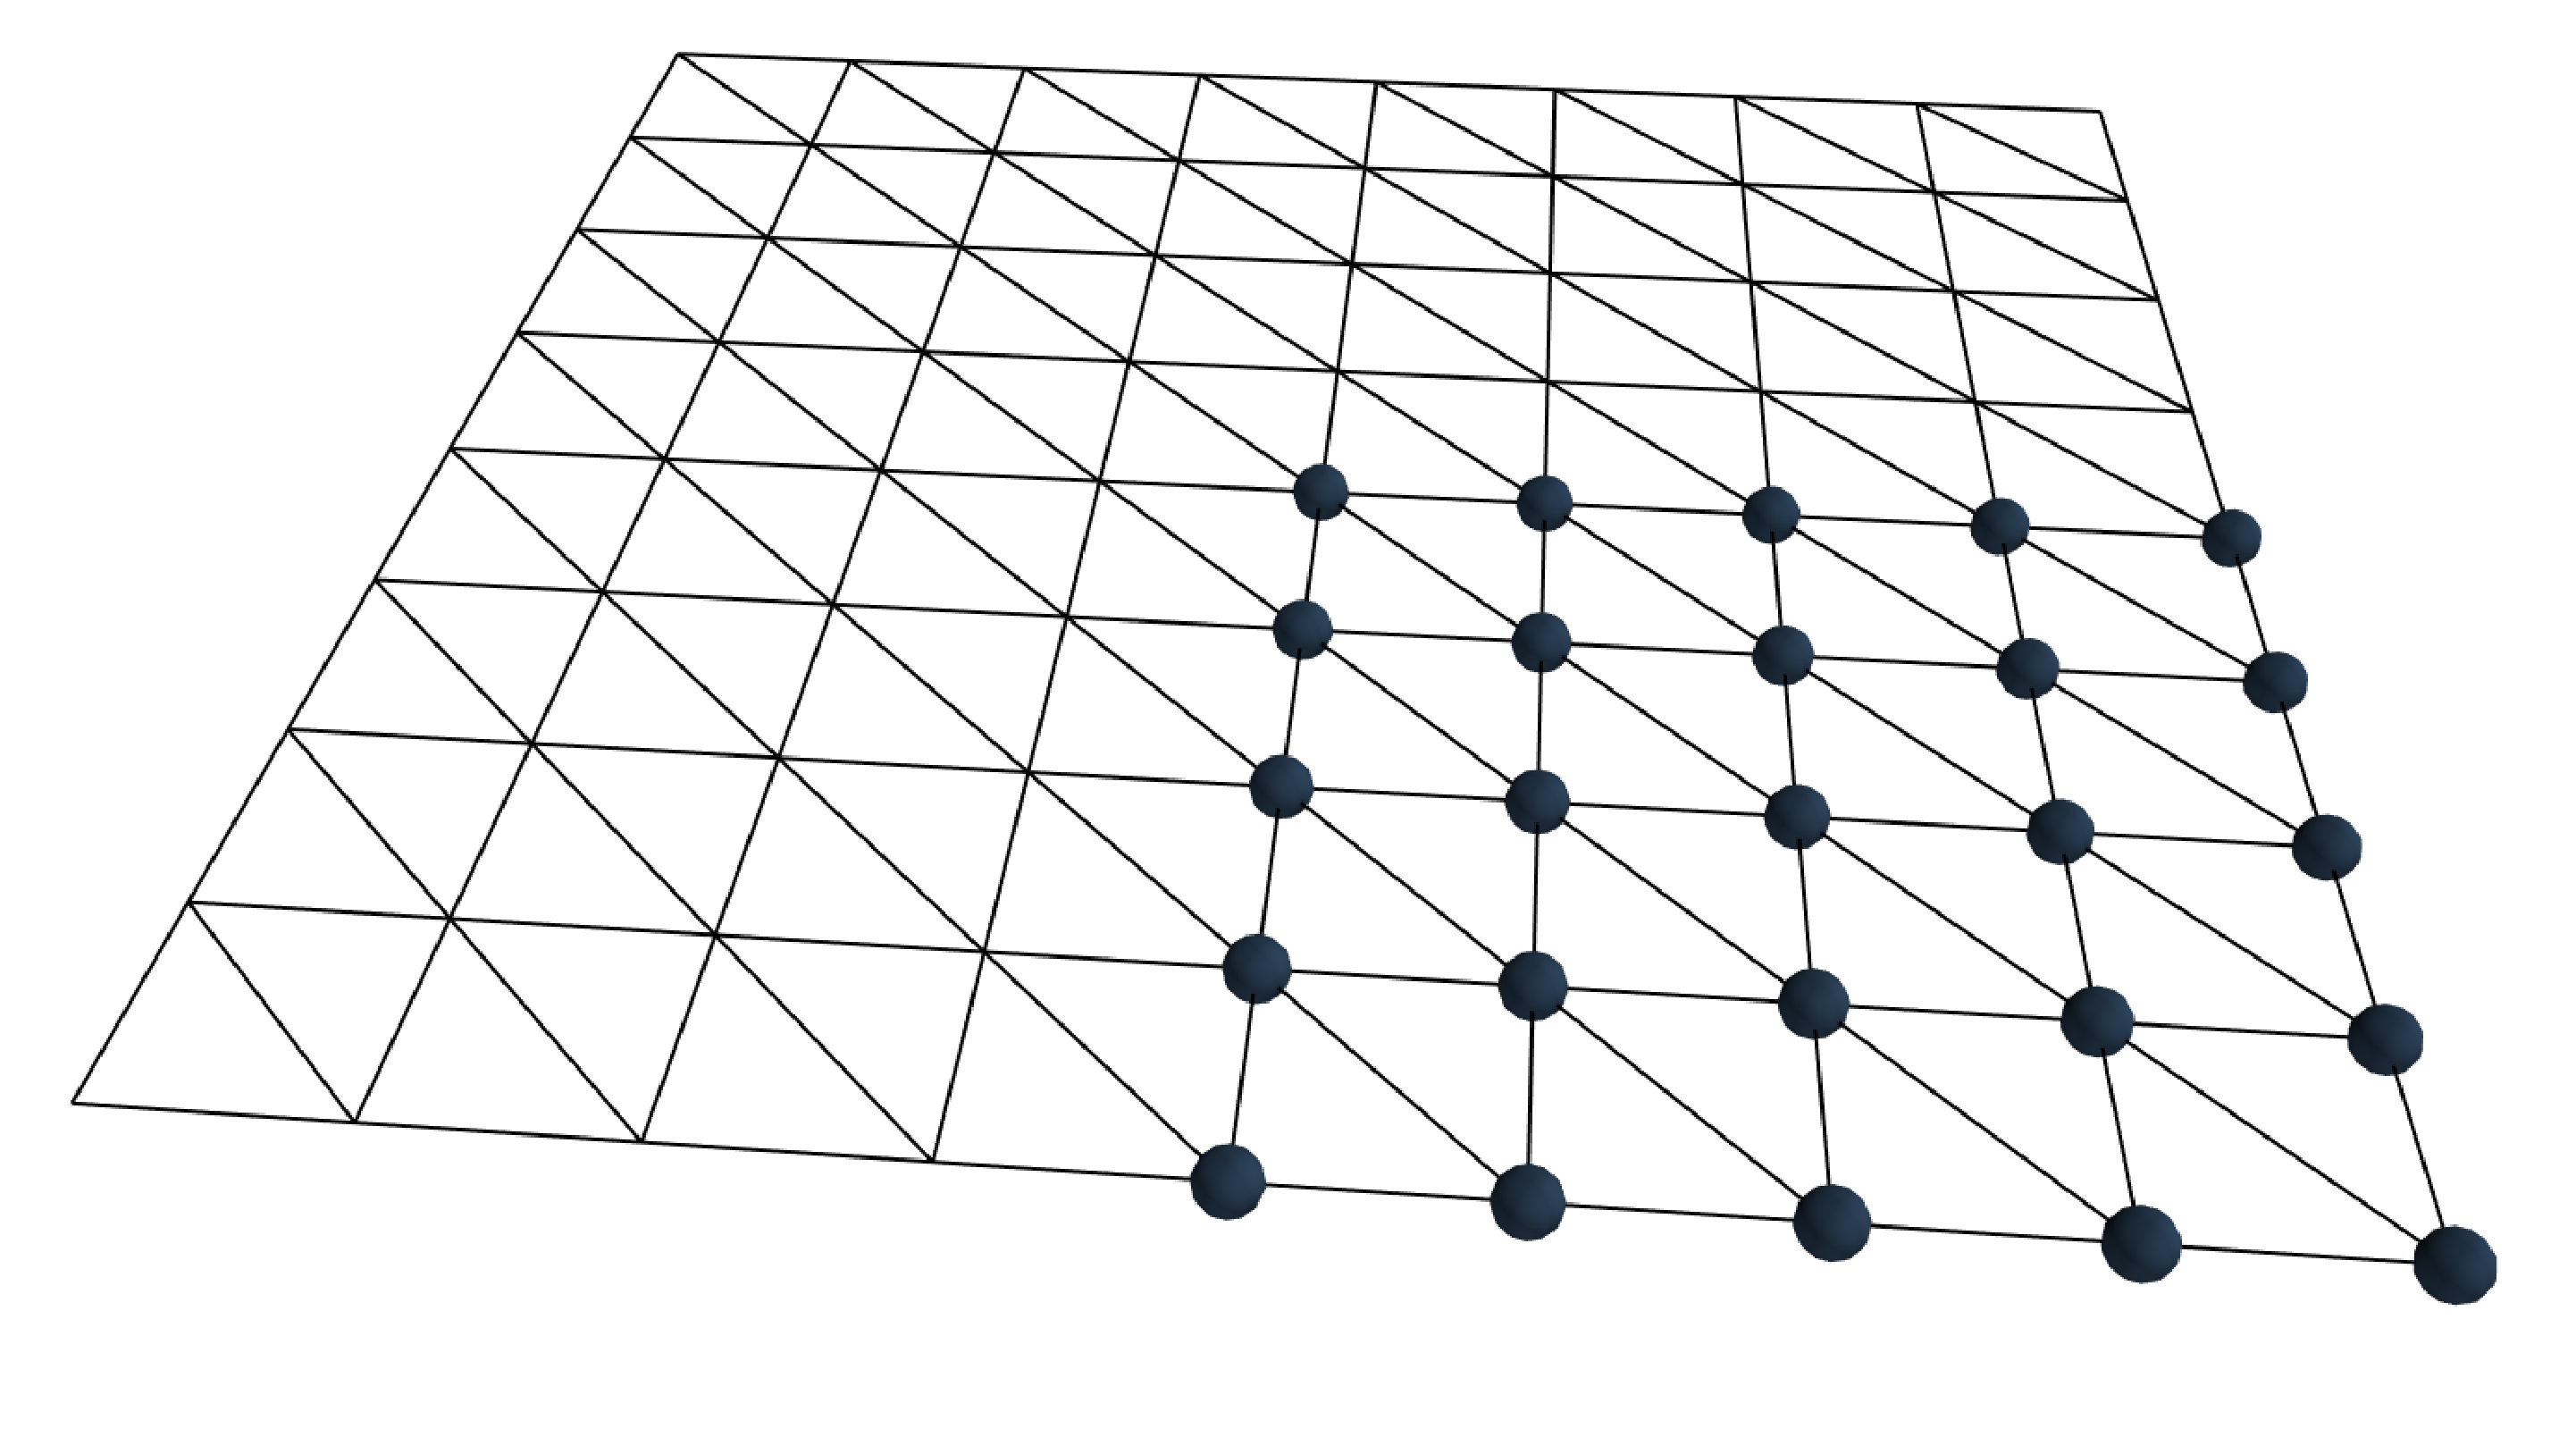
\includegraphics[width=0.22\textwidth]{images/dofmeshes/correct/dofs_k_0_lvl_l2.pdf}};

\node (B3) at (\xB, \yThree)
    {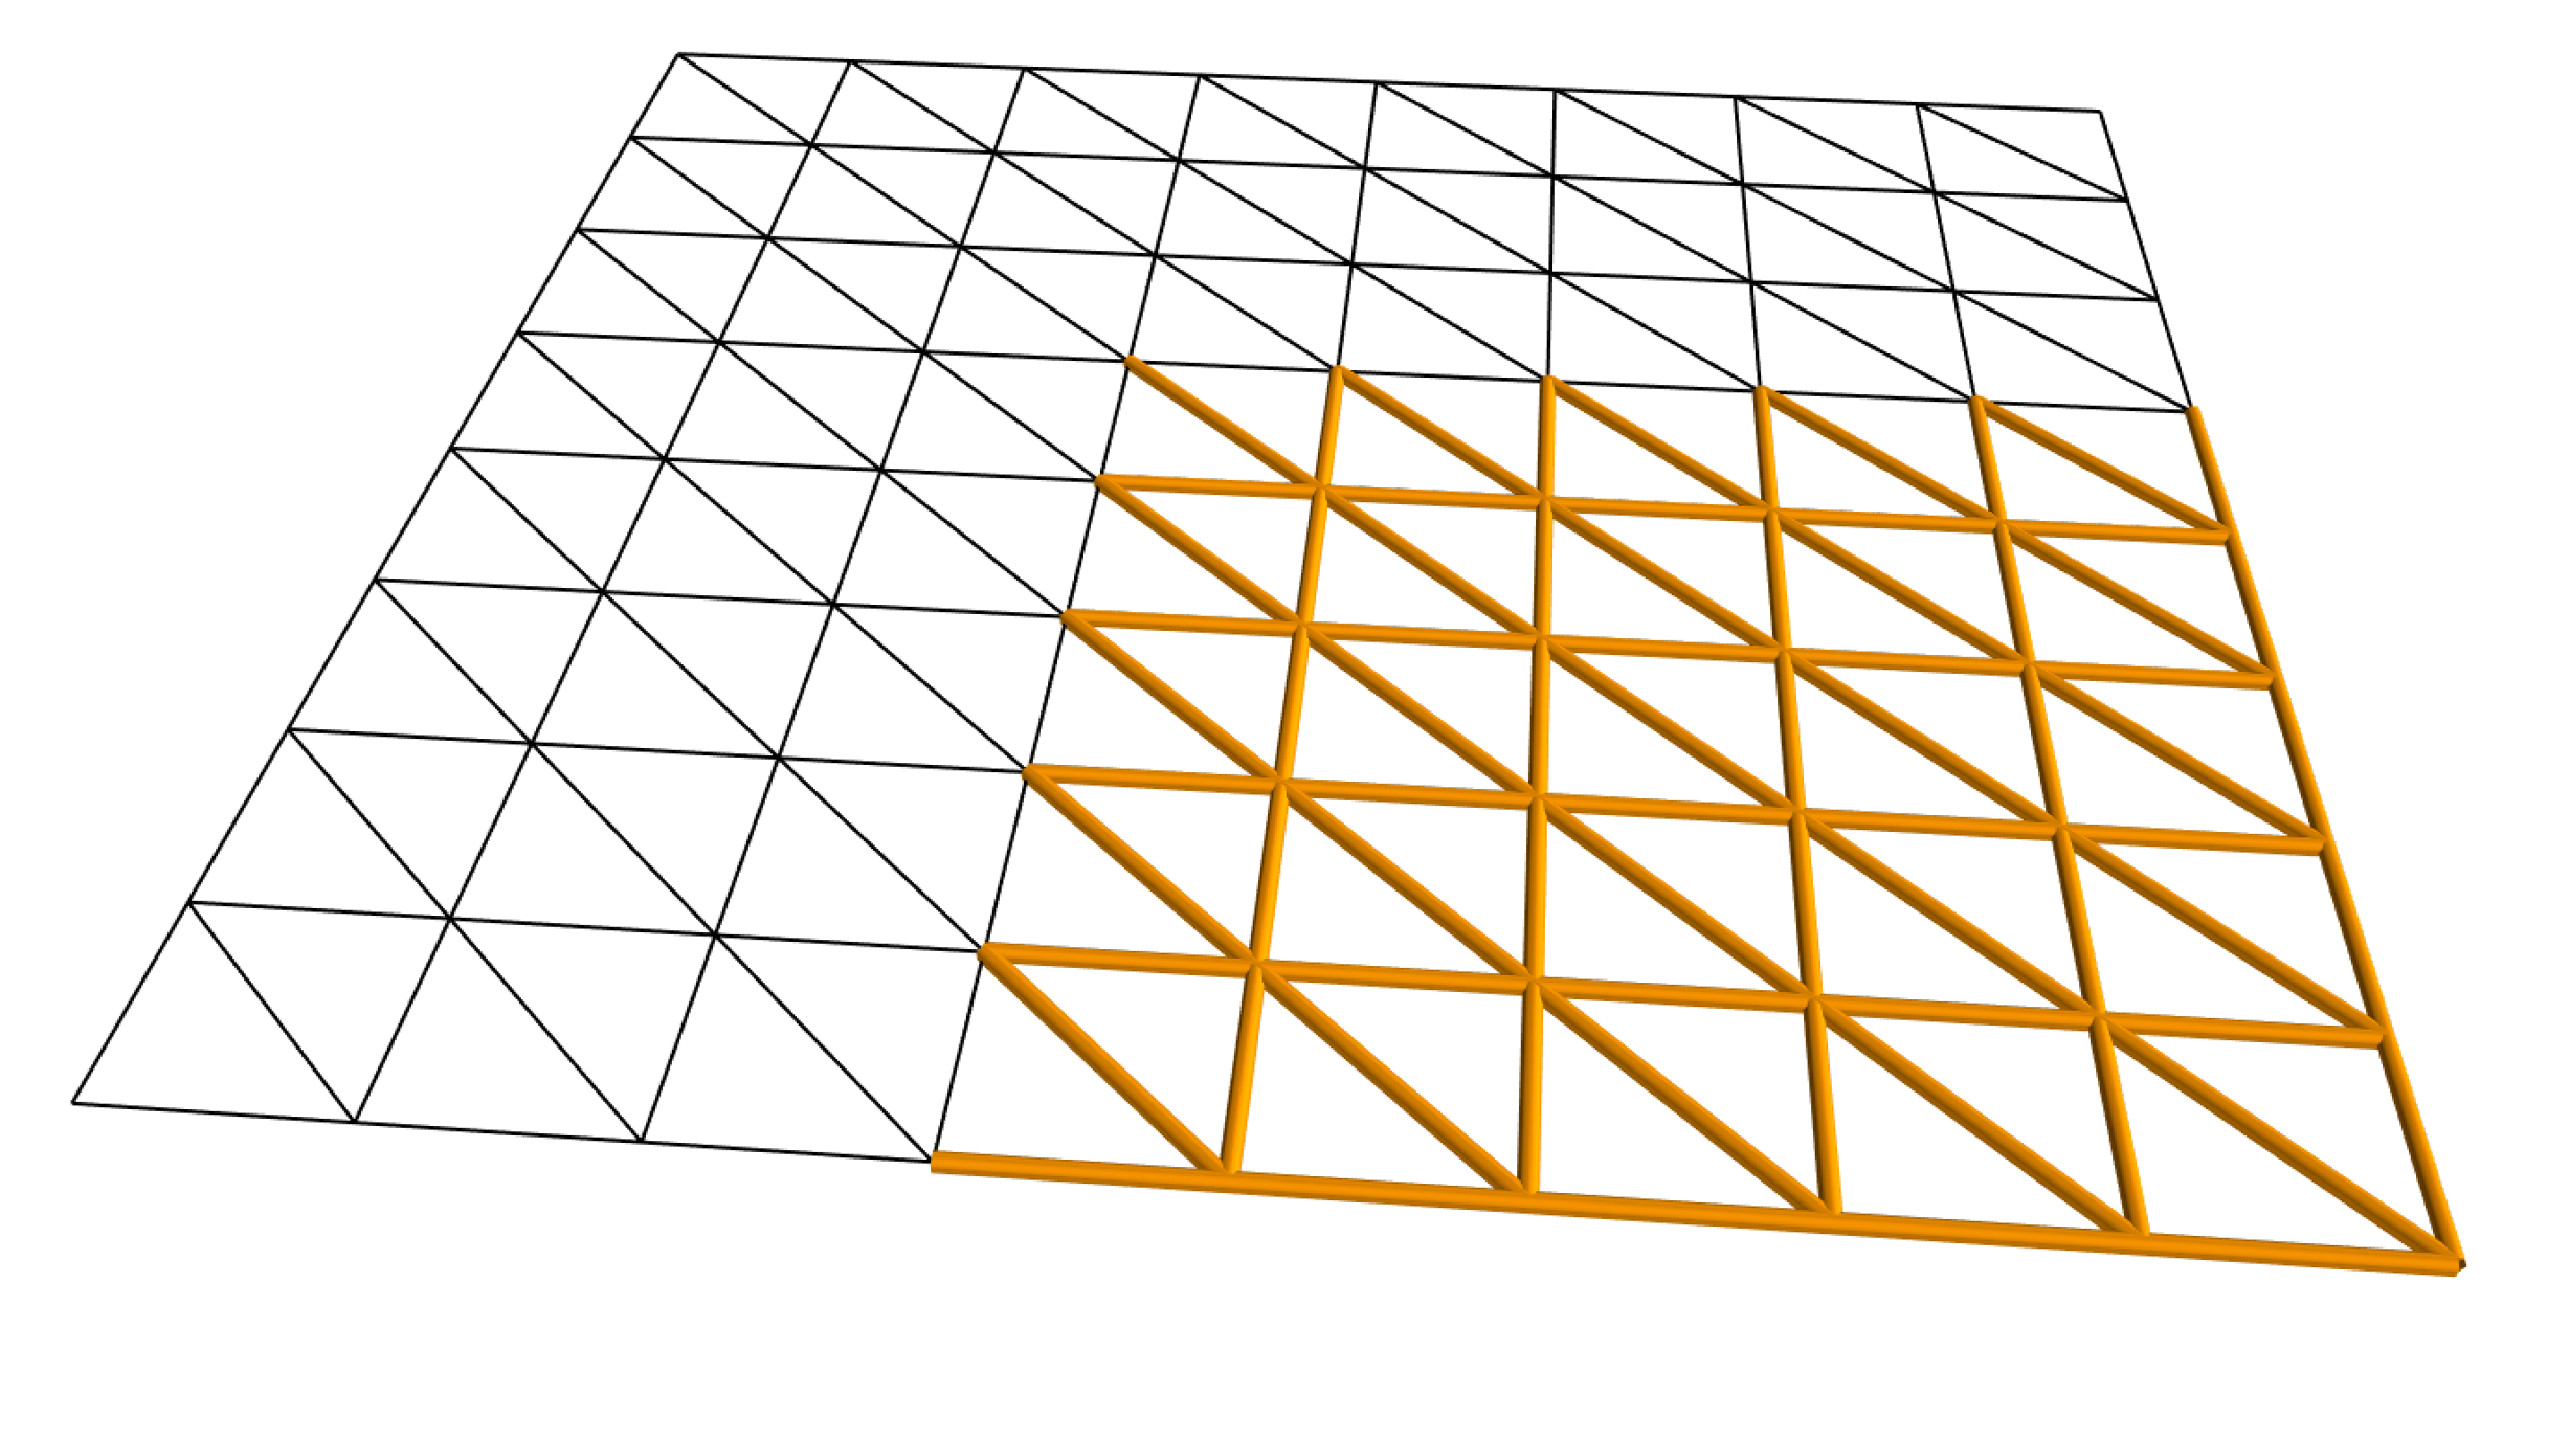
\includegraphics[width=0.22\textwidth, trim=10pt 0pt 10pt 0pt, clip]{images/dofmeshes/correct/dofs_k_1_lvl_l2.pdf}};

\node (C3) at (\xC, \yThree)
    {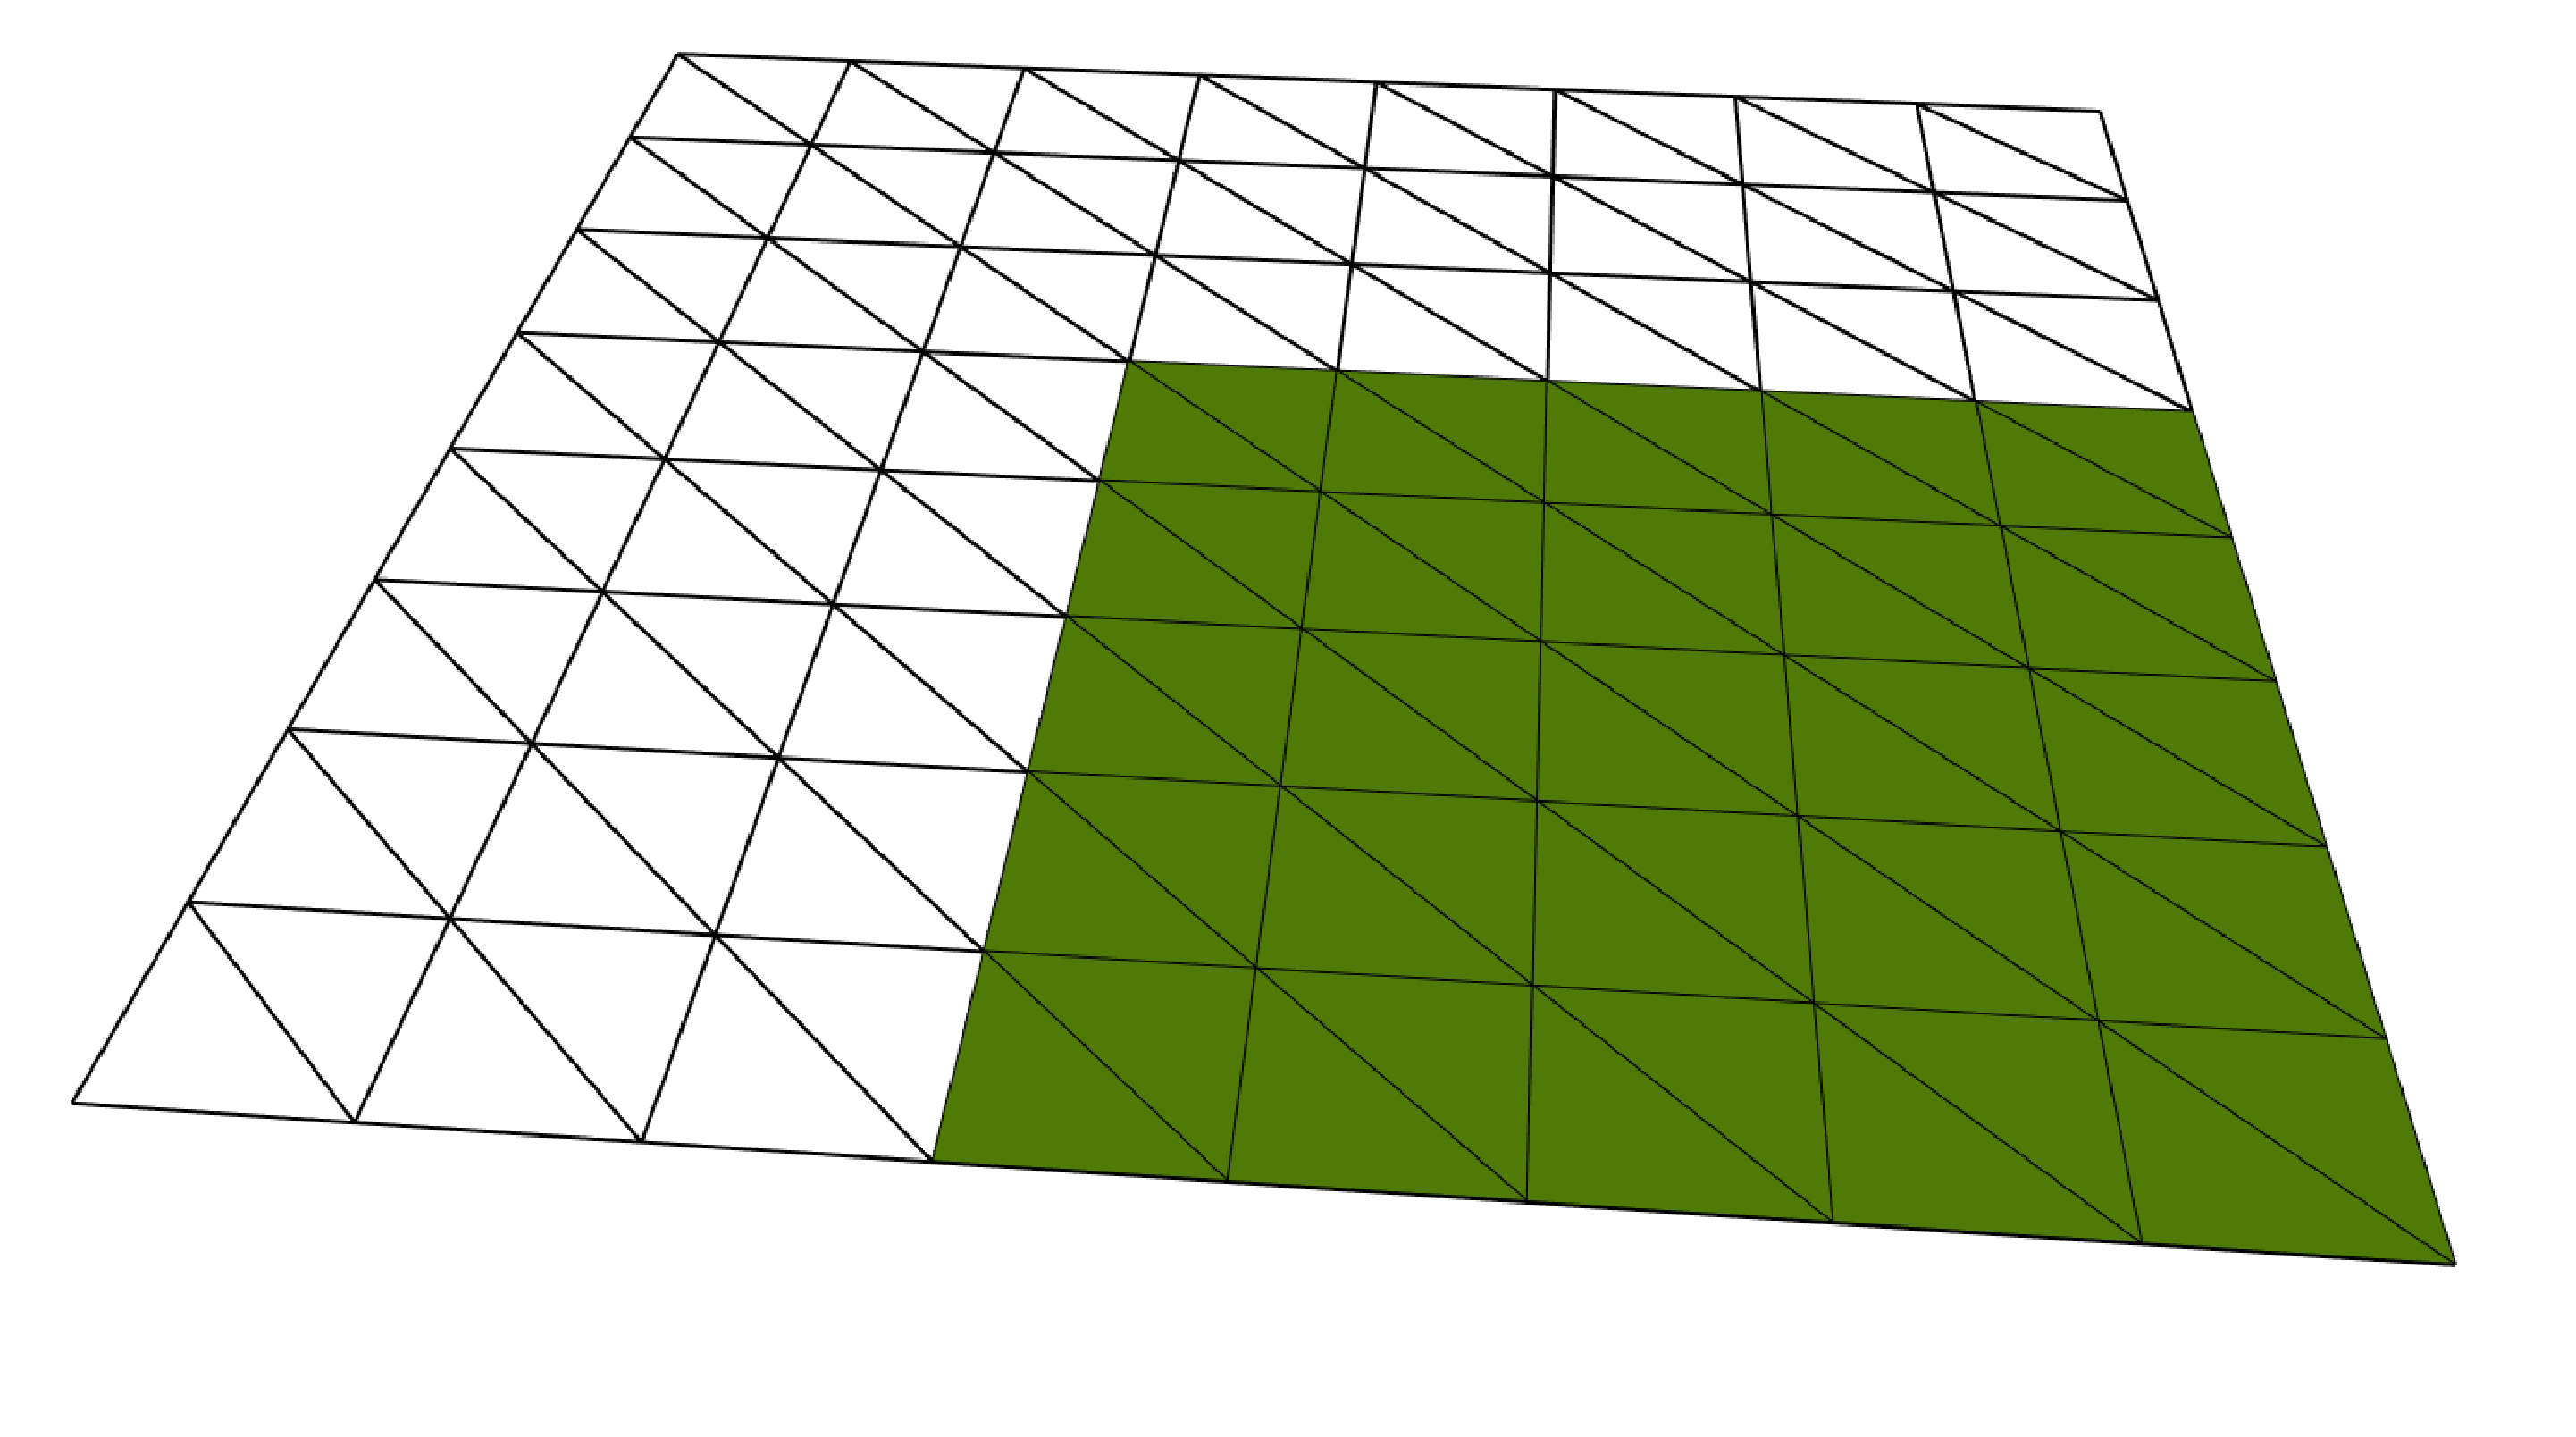
\includegraphics[width=0.22\textwidth]{images/dofmeshes/correct/dofs_k_2_lvl_l2.pdf}};

\node[above=8pt of A1, font=\bfseries, inner sep=2pt] (colA) {$k = 0$};
\node[above=8pt of B1, font=\bfseries, inner sep=2pt] (colB) {$k = 1$};
\node[above=8pt of C1, font=\bfseries, inner sep=2pt] (colC) {$k = 2$};

\node[left=12pt of A1, font=\bfseries, inner sep=2pt] {$\l = 0$};
\node[left=12pt of A2, font=\bfseries, inner sep=2pt] {$\l = 1$};
\node[left=12pt of A3, font=\bfseries, inner sep=2pt] {$\l = 2$};

\draw[
    decoration={brace, amplitude=6pt, raise=4pt},
    decorate, line width=1.2pt
]
    (A1.north west|-colA.north) -- (C1.north east|-colA.north)
    node[midway, above=14pt, font=\bfseries] {Active DoFs};

\node (topfig) at (3.9cm, 4.0cm)
    {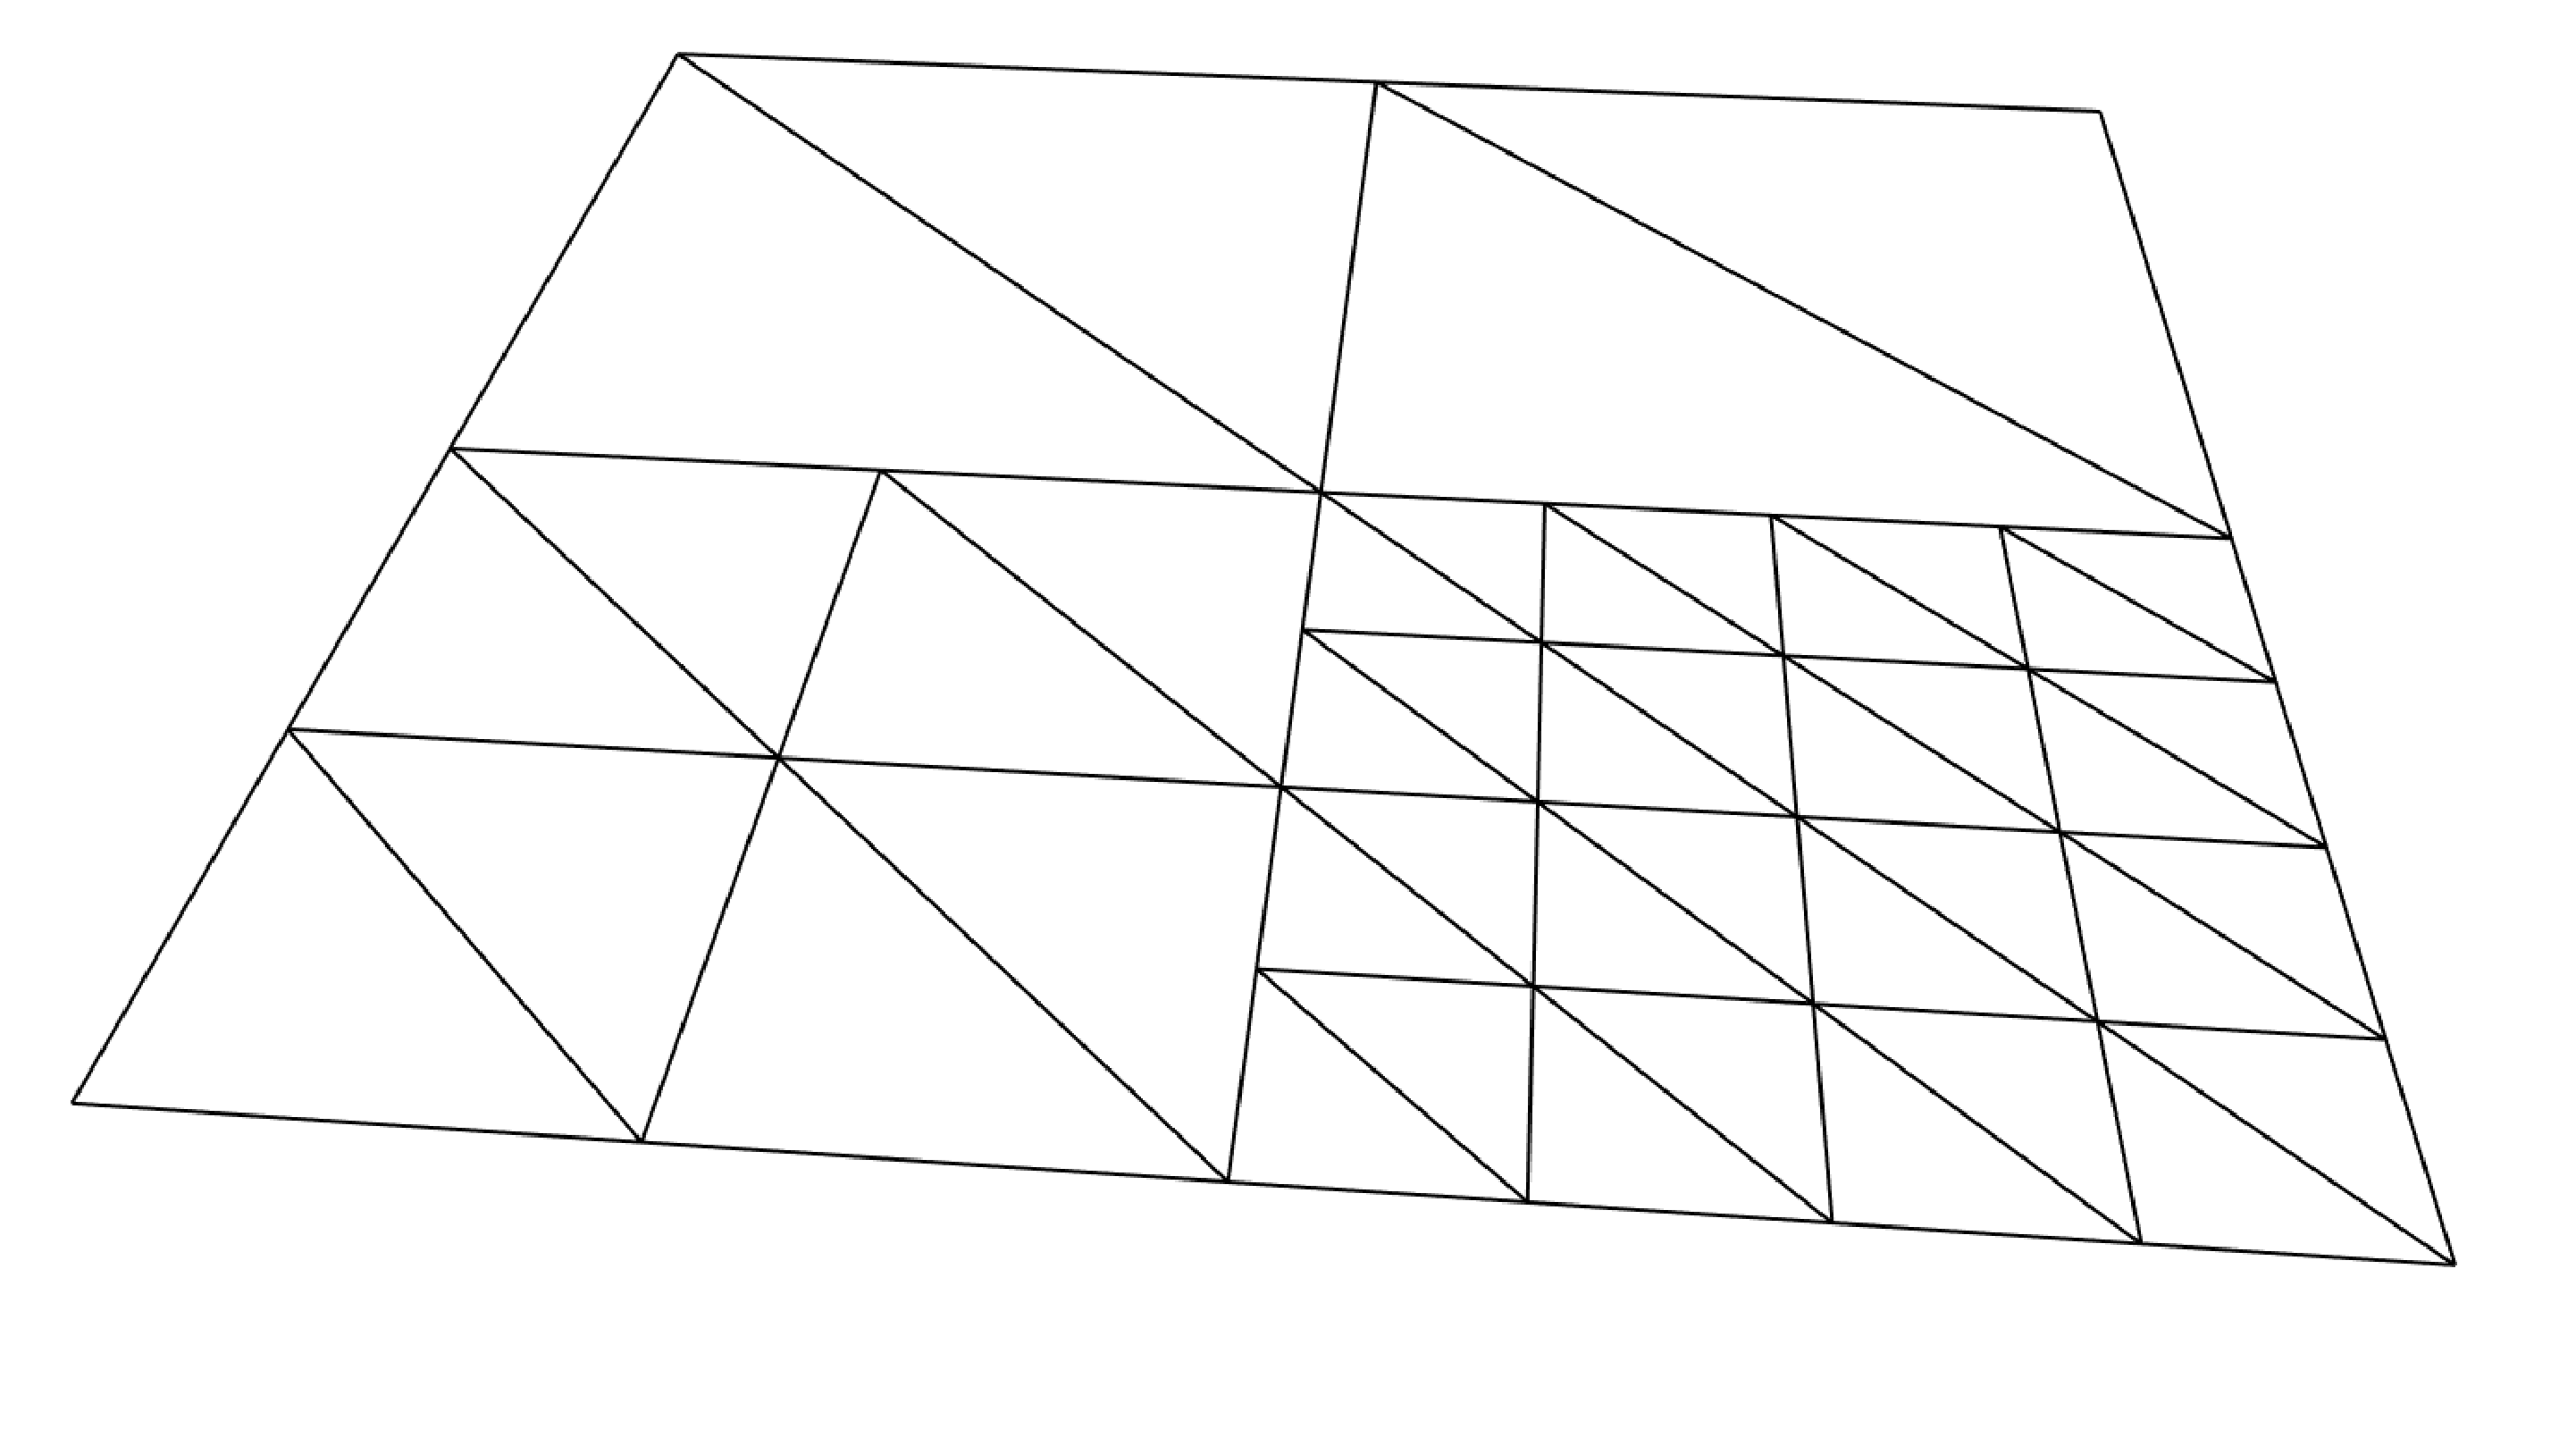
\includegraphics[width=0.3\textwidth]{images/dofmeshes/correct/subdiv_partition.pdf}};

\node[above=6pt of topfig, font=\bfseries] {Subdivision partition};

\end{tikzpicture}
\end{center}
\caption{Active $k$-form DoFs for the three-level subdivision partition shown at top. Columns correspond to form degree $k = 0$ (vertices, dark circles), $k = 1$ (edges, orange), and $k = 2$ (faces, green). Rows correspond to active DoFs at levels $\l = 0$, $1$, $2$ respectively.}
\label{fig:active_dofs}
\end{figure}

\FloatBarrier

\section{Exactness of the resulting Sequence of Spaces}

\subsection{The goal}

We aim to adapt the argument of \cite{Evans.2020} in the case of hierarchical B-splines to our adaptive subdivision-induced complex. Due to the similarity of our frameworks, the following lemma in their work provides a good starting point:

\begin{lemma}[Lemma 5.5 in \cite{Evans.2020}, adapted]
    \label{lemma:isomorphism_on_cohomology}
    The complex $(\hierSDFspace{k}{\C_{\leq \l}}{\L}, \extd)$ of adaptive subdivision $k$-form spaces for $\l = 1,\dots, L$ is exact if and only if the inclusion map $j: X_{\l,\l+1} \to X_{\l+1, \l+1}$ induces an isomorphism between the cohomology groups $H^k(X_{\l,\l+1})$ and $H^k(X_{\l+1,\l+1})$ for $k=1,2$.
\end{lemma}

Just like in \cite{Evans.2020}, the spaces $X_{\l,\l+1}$ and $X_{\l+1, \l+1}$ represent the coarse space that is removed and the fine space that is added at level $\l+1$. Concrete examples for primitive subdivision partitions will follow.

\subsection{Our preliminary result}

\begin{assumption}
    \label{ass:exact_partition}
    The subdivision partition is \emph{exact}, i.e. refined patches are unions of vertex stars (all faces around a vertex).
\end{assumption}

The following investigation of primitive configurations will contain examples of partitions that do or do not satisfy this assumption. The partition in Figure~\ref{fig:active_dofs} does not satisfy the assumption yet the adaptive spaces defined on it constitute an exact sequence.

The next theorem formally states the kind of result we want to achieve after restricting ourselves to exact subdivision partitions.

\begin{theorem}
    Let $\C$ be an exact subdivision partition of the mesh $\T_\L$. The adaptive subdivision $k$-form spaces $\hierSDFspace{k}{\C}{\L}$ then constitute the exact sequence
    \begin{equation}
    \begin{tikzcd}
        0 \arrow[r] & \mathbb{R} \arrow[r, "\subset"] & \hierSDFspace{0}{\C}{\L} \arrow[r, "\extd"] & \hierSDFspace{1}{\C}{\L} \arrow[r, "\extd"] & \hierSDFspace{2}{\C}{\L} \arrow[r] & 0.
    \end{tikzcd}
    \end{equation}
\end{theorem}

Additionally, we would need a similar version of the exact sequence for the spaces with vanishing trace boundary conditions.

\subsection{Draft of a proof}

The key difference between the HB-spline complexes and the subdivision complexes is how the domain decomposition parameterises the respective spaces. Fine HB-spline basis functions are inserted once their support is entirely contained in the domain $\Omega_{\l+1}$ that is refined. In this way, it is more "conservative" than the subdivision spaces that add fine basis functions for every vertex in the fine patch, even on the boundary.

We could re-cast our selection method into the HB-spline framework by extending the refined patch to cover the support of all fine basis functions. In general, describing this extended patch is only simple once a set of active DoFs has been chosen. Before that, it is quite hard to quantify their supports.

%We generally do not need to distinguish between the B\'ezier mesh and the Greville mesh because they coincide in our framework. In the case of B-splines, we can think of $p_1 = p_2 = 3$, in which case the Greville sites correspond to the B\'ezier mesh vertices, edges and faces one to one.

\subsubsection{Refinement across one level.}

Starting from the uniform complex of subdivision differential form spaces at level $\lzero$, we can build the adaptive spaces by refining level by level. Lemma~\ref{lemma:isomorphism_on_cohomology} tells us that we need to look at the coarse spaces that are removed and the fine spaces that are added during refinement and check whether they have the same cohomology. There are only a handful of cases to consider in the subdivision case.

\paragraph{Two patches meeting in a single vertex.}

This is the critical case. The two refined patches share only one vertex and no edges, see Figure~\ref{fig:single_vertex_shared}. In this case, we remove a coarse space with effectively two distinct connected components and insert a fine space with only one connected component. Hence, the cohomologies mismatch and the Euler characteristic changes from $2$ to $1$. Ultimately, that means that Lemma~\ref{lemma:isomorphism_on_cohomology} does not hold in this case. Note that this configuration is ruled out by Assumption~\ref{ass:exact_partition}.

\begin{figure}[H]
\centering
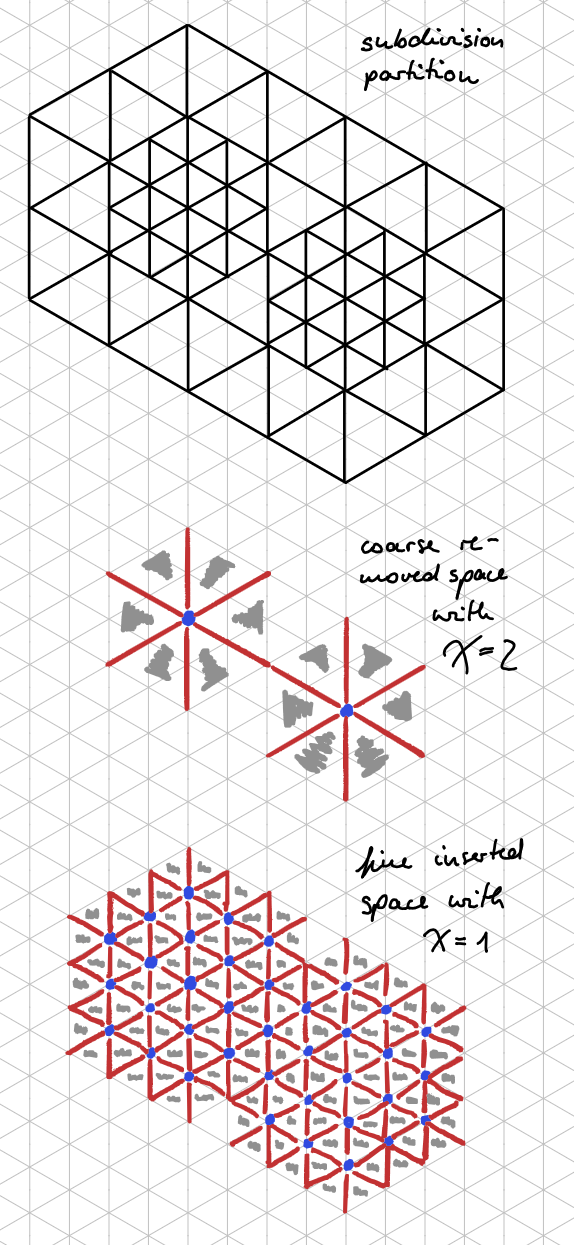
\includegraphics[width=0.5\textwidth]{configurations/two_patches_touching_in_vertex.png}
\caption{Top: the local subdivision partition. Middle: the coarse removed space $X_{\ell,\ell+1}$. Bottom: the fine inserted space $X_{\ell+1,\ell+1}$. Blue vertices, red edges and grey faces indicate the active DoFs.}
\label{fig:single_vertex_shared}
\end{figure}

\paragraph{Two patches touching along an edge.}

In this configuration, two coarse patches share an edge. Note that the common edge is also part of the coarse removed space. The coarse and fine spaces have the same Euler characteristic of $1$. I also think they have the same cohomology since the centre edge forces the $2$-form harmonics (constant $2$-forms in the relative de Rham complex) to coincide for the two coarse patches but I am not entirely sure. This configuration does not seem problematic then, but it is still ruled out by Assumption~\ref{ass:exact_partition}.

\begin{figure}[H]
\centering
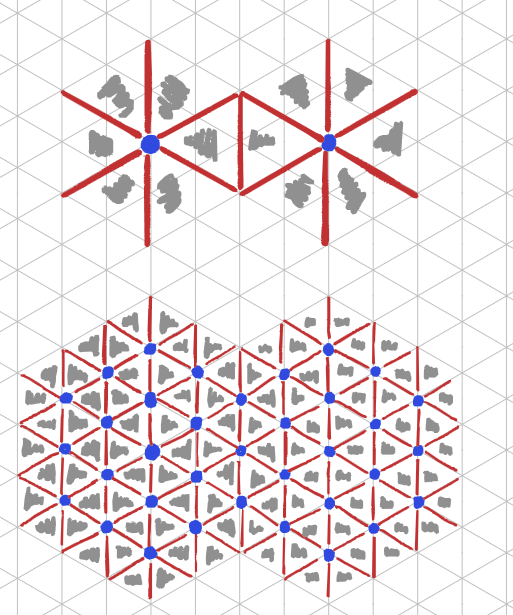
\includegraphics[width=0.5\textwidth]{configurations/two_patches_touch_in_edge.png}
\caption{Top: the coarse removed space for the edge-touching configuration; two vertex stars sharing an edge. Bottom: the corresponding fine inserted space.}
\end{figure}

\paragraph{Two patches sharing one or more faces.}

The two patches can be combined into one, implying that there is no problem.

\paragraph{Vertex hole in a patch.}

This configuration is the smallest possible configuration that has a non-trivial topology since it has a hole. Thus, its Euler characteristic is $0$. The refined space (only vertices are drawn) is simply connected again, so the cohomology has changed and the Euler characteristic is $1$ again. The configuration might still not be problematic because the basis function associated to the (remaining) hole vertex is now linearly dependent which should fix the overall cohomology of the whole space. Note that the way we select active DoFs does not allow this configuration to occur.

\begin{figure}[H]
\centering
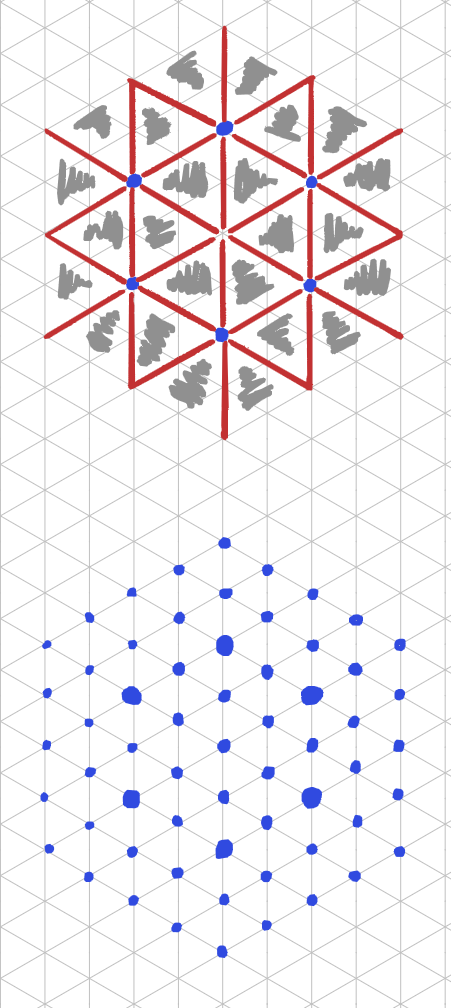
\includegraphics[angle=90, width=\textwidth]{configurations/center_vertex_missing.png}
\caption{Left: coarse removed space. Right: inserted fine space (only vertices drawn, all adjacent edges and faces are active).}
\end{figure}

\paragraph{Edge hole in a patch.}

Same as vertex hole and cannot occur due to DoF selection.

\begin{figure}[H]
\centering
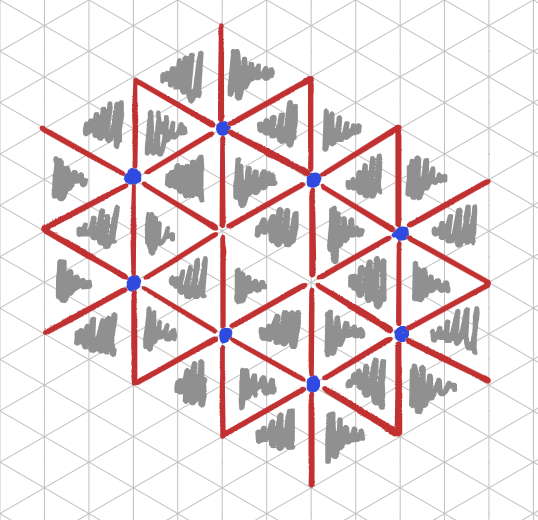
\includegraphics[width=0.55\textwidth]{configurations/center_edge_and_vertices_missing.png}
\caption{The coarse removed space with a central edge and its endpoint vertices deactivated.}
\end{figure}

\paragraph{Face hole in a patch.}

This configuration can theoretically occur with our DoF selection algorithm. However, the coarse face in the centre violates Assumption~\ref{ass:exact_partition}.

The Euler characteristic changes from $0$ to $1$ for the individual spaces but there are also multiple linearly dependent basis functions now. The same is true for any ``narrow strip'' of faces (where all edges of the faces are also edges on the patch boundary).

\begin{figure}[H]
\centering
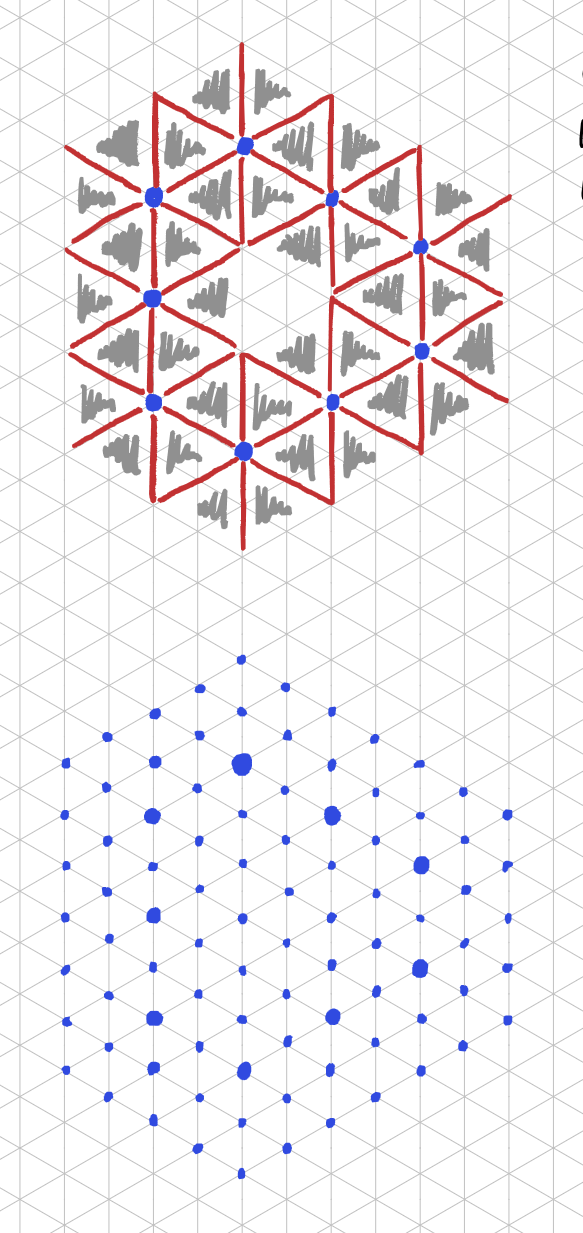
\includegraphics[angle=90, width=\textwidth]{configurations/center_face_missing.png}
\caption{Left: coarse removed space. Right: inserted fine space (only vertices drawn, all adjacent edges and faces are active)}
\end{figure}

\paragraph{Vertex star hole in patch.}

This configuration is the smallest possible configuration in which both the coarse and fine space share the same non-trivial topology. This case is not ruled out by the DoF selection or Assumption~\ref{ass:exact_partition}. This case is not problematic and generalizes to larger holes (as long as the hole is the union of vertex stars) and multiple holes.

\begin{figure}[H]
\centering
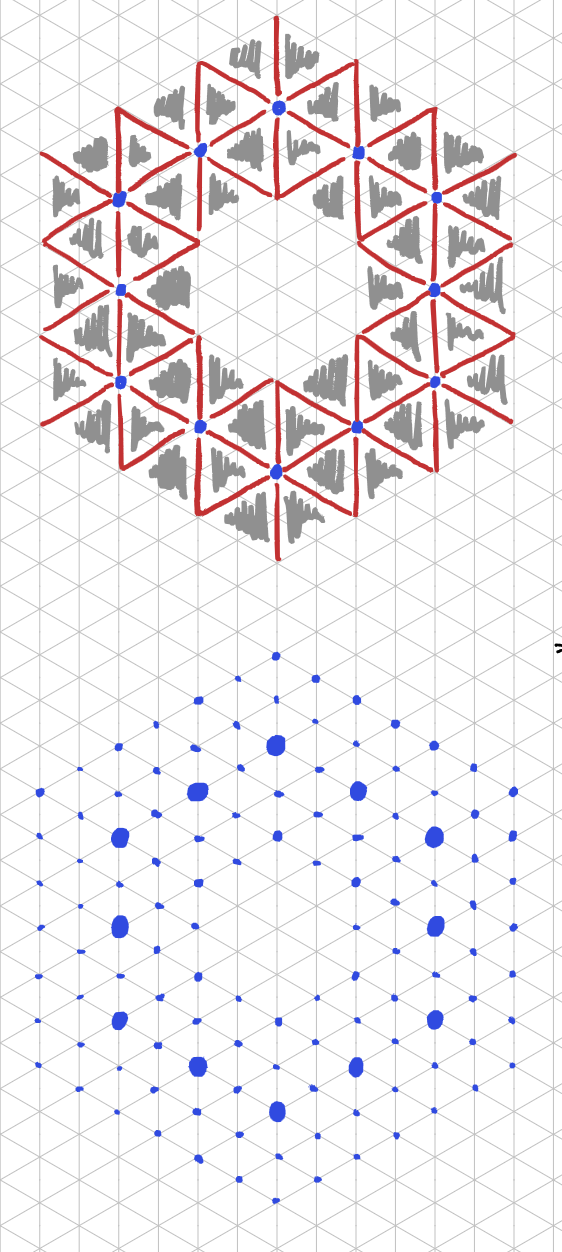
\includegraphics[angle=90, width=\textwidth]{configurations/center_vertex_star_missing.png}
\caption{Left: coarse removed space. Right: inserted fine space (only vertices drawn, all adjacent edges and faces are active)}
\end{figure}

\subsubsection{Multi-level refinement}

Our framework allows refinement across multiple levels. We can think of that as applying single-level refinement twice to the same patch. In our construction, this implies additional ``interface'' DoFs, see Figure~\ref{fig:active_dofs} (level 1 simplices on the interface between the patches on levels 0 and 2). 

The composition of multiple single-level refinement steps also implies that the configurations from above apply and we do not get any additional problematic cases. For example, for the case of a single shared vertex, the ``severity'' of the cohomological mismatch increases.

\bibliography{references}

\end{document}
